\documentclass[runningheads]{llncs}

\usepackage[ruled,vlined,linesnumbered,norelsize]{algorithm2e}
\usepackage{amsmath,amssymb}
\usepackage[T1]{fontenc} % font encoding; recommended by LNCS template
\usepackage{graphicx}
\usepackage{hyperref}
\usepackage[misc]{ifsym} % letter symbol to mark corresponding author
\usepackage{pifont}
\usepackage{siunitx}
\usepackage{subcaption}
\usepackage{tablefootnote}
\usepackage{tabularx}
\usepackage[table]{xcolor}
\usepackage{tikz} % has to be loaded after "xcolor" here, else "option clash"

\newcommand{\cmark}{\ding{51}} % symbols for table comparing benchmarking approaches
\newcommand{\xmark}{\ding{55}}

\DontPrintSemicolon % configuration for algorithm2e
\def\NlSty#1{\textnormal{\fontsize{8}{10}\selectfont{}#1}}
\SetKwSty{texttt}
\SetCommentSty{emph}

\renewcommand\UrlFont{\color{blue}\rmfamily} % link coloring according to LNCS template

\begin{document}

\title{Active Learning for SAT solver Benchmarking}

\author{
	Tobias Fuchs\orcidID{0000-0001-9727-2878} (\Letter) \and \\
	Jakob Bach\orcidID{0000-0003-0301-2798} \and \\
	Markus Iser\orcidID{0000-0003-2904-232X}
}

\institute{
	Karlsruhe Institute of Technology (KIT), Karlsruhe, Germany \\
	\email{info@tobiasfuchs.de, jakob.bach@kit.edu, markus.iser@kit.edu}
}

\authorrunning{T. Fuchs et al.} % according to sample paper of template: first names are abbreviated; if there are more than two authors, 'et al.' is used.

\maketitle

\begin{abstract}
  Experimentation, in particular the evaluation of the runtime of a concrete implementation, is one of the most important phases in the development of algorithms.
  This also applies to solutions of the SAT problem (propositional sat\-is\-fia\-bi\-li\-ty).
  While the field of SAT solver benchmarking is well established, traditional benchmark selection approaches do not optimize for benchmark runtime.
  Benchmark compilation selects representative instances from a pool of instances such that they reliably discriminate SAT solvers based on their runtime.
  In this paper, we present an active learning based dynamic benchmark selection approach that predicts the rank of a new solver among its competitors with minimum running time and maximum rank prediction accuracy.
  We evaluated this approach using the Anniversary track dataset from the 2022 SAT Competition. 
  Our dynamic instance selection approach can predict the rank of a new solver after about \SI{10}{\%} of the time it would take to run the solver on all instances of this dataset, with a prediction accuracy of about \SI{92}{\%}. 
  In this paper, we also discuss the importance of instance families in the selection process. 
  Our tool provides a reliable way for SAT solver engineers to efficiently determine the performance of a new SAT solver.

  \keywords{Propositional satisfiability \and Benchmarking \and Active learning}
\end{abstract}


\section{Introduction}
\label{sec:intro}
One of the main phases of algorithm engineering is benchmarking.
This is also true for the pro\-po\-si\-tio\-nal sat\-is\-fia\-bi\-li\-ty problem (SAT), the archetypal $\mathcal{NP}$-complete problem.
While state-of-the-art solvers embark upon more and more problem instances, SAT solver evaluation is steadily getting more costly.
Competitive SAT solvers are the result of extensive experimentation and a variety of ideas and considerations~\cite{FroleyksHIJS21,sat2022}.
While the field of SAT solver benchmarking is well established, traditional benchmark selection approaches do not optimize for benchmark runtime.
The goal of traditional approaches is to select a representative set of instances for ranking solvers based on a scoring scheme~\cite{Gelder11,HoosKSS13}.
SAT~Competitions typically use the widely adopted PAR-2 score, i.e, the average runtime with a penalty term of $2 \tau$ for timeouts with time-limit $\tau$~\cite{FroleyksHIJS21}.

In this paper, we present a novel active learning based benchmark selection approach which is able to predict the rank of a new solver with high accuracy in only a fraction of the time needed to evaluate the full benchmark.
The problem we solve is specified in Definition~\ref{def:new-solver-problem}.

\begin{definition}[New-Solver Problem]
	Given a pool of instances~$\mathcal{I}$, solvers~$\mathcal{A}$, and runtimes~$r\!: \mathcal{A} \times \mathcal{I} \rightarrow \left[0, \tau\right]$ with time limit $\tau$, maximize the confidence in predicting the rank of a new solver $\hat{a} \notin \mathcal{A}$ while minimizing the total benchmark runtime by incrementally selecting instances in $\mathcal{I}$ to evaluate $\hat{a}$.
	\label{def:new-solver-problem}
\end{definition}

%Note that we know the runtimes of all solvers, except the new one, on all instances.
%There also is work on collaborative filtering, where runtimes are only partially known, for algorithm selection~\cite{misir2017alors,misir2017data}.
%MI: this belongs to discussion of related work

%We predict the solver ranking induced by this scoring, without predicting exact solver runtimes.

%This allows for both comparing the solvers as well as identifying solvers with similar behavior if looking at individual predictions per instance.
%JB: is there any further behavior we can deduce about a solver scoring apart from a performance ranking? "similar behavior" could IMHO be something like two solvers being fast/slow on the same instances, but that cannot be deduced from overall score
%TF: made it clearer
%MI: makes no sense in the context

% The following belongs to Related Work discussion... already references the table there... will fuse / rework tomorrow
Our algorithm is unique in that it is the only one, to the best of our knowledge, that has all of the following features (also refer to Table~\ref{tab:requirements}).
Our benchmarking process outputs a \emph{ranking} to compare the new solver against the existing set of solvers as described above.
We optimize the \emph{runtime} that our strategy needs to arrive at its conclusion.
We use problem-instance and runtime \emph{features} $\varphi\!: \mathcal{A} \times \mathcal{I} \rightarrow \mathbb{R}^n$ since such features already have proven to be helpful in classic benchmark-set-selection approaches~\cite{HoosKSS13} as well as in portfolio selection~\cite{CollauttiMMO13,NgokoCT19}.
%JB: I think we can remove this criterion, as it also is satisified by all competitors (and is commented out in table; if we keep criterion, we should also show it in table)
%TF: I still find it worth mentioning. So, I added it back to the table.
Moreover, we select instances \emph{non-randomly} and \emph{incrementally}.
By doing so, we have a greater impact on the properties of the benchmarking approach such as its required runtime.
Sampling instances incrementally means taking runtime information from already done experiments into account when choosing the next.
Rather than solely outputting a binary classification, i.e, the new solver is worse than solver A, we provide a \emph{scoring function} that shows by which margin a solver is worse and how similar it is to existing approaches (\emph{comparability}).
%JB: we should rename the "interpretability" criterion (make it more specific), term "interpretability" can have lots of different meanings and our specific meaning is not very intuitive
%TF: Renamed it to "comparability"
Finally, our strategy incrementally selects only a single benchmark set to compare one new solver $\hat{a}$ with the set of existing solvers $\mathcal{A}$ whose cardinality can be any number (\emph{scalability}).
%JB: for what do we measure cost here?
%TF: made it clearer
We avoid comparing pairs of solvers, which requires a non-constant number of benchmark sets.
%JB: need to discuss this; logarithmic (compare one-vs rest) / log-linear (compare each pair) effort might be sufficient if the binary-search-/recursive-sorting-like procedure used
%TF: "non-constant number of benchmark sets"
Since a new solver idea is rarely best on the first try but requires more or less tweaking, it is desired to obtain a solver ranking fast.
In this way, a new solver idea can be discarded if it performs poorly across the board or may be further tweaked if it shows promising results at least in some cases.

To sum up our contribution, we take the SAT Competition~2022 Anniversary Track benchmark~\cite{sat2022} (5355 instances, full runtimes of 28 solvers), perform cross-validation by treating each solver as new once, and predict these solvers' PAR-2 rank with about \SI{92}{\%} accuracy with only about \SI{10}{\%} of the runtime that would be needed to evaluate these solvers on the complete set of instances.
Both results are averages across all cross-validation iterations.
%JB: I think we should expand a bit more on experimental design (how many instances/solvers, what do we compare), and the key results; I think it's okay if the intro becomes a bit longer (and in turn, the overview of the approach's features can be cut a bit)
%TF: added a bit more information

For reproducibility, all our source code\footnote{temporary, anonymized version for review: \url{xxx}} and and data\footnote{temporary, anonymized version for review: \url{xxx}} are available on GitHub.


\section{Related Work}
This section discusses work in several related fields.
First, we take a look at traditional SAT solver benchmarking.
Second, we explore how SAT solver configuration systems deal with navigating possible configurations.
Third, we discuss an existing benchmark-set-selection approach that optimizes for benchmark runtime.
Finally, we show how active-learning techniques can help to tackle the aforementioned \emph{New-Solver Problem}.

Table~\ref{tab:requirements} shows a concise overview of existing approaches with a related goal.
%JB: we can probably cut this part a bit, as we discuss weaknesses of individual approaches later anyway
%TF: it's supposed to be a short overview of what is to come
While traditional benchmark-set-selection~\cite{HoosKSS13} lacks the aspect of runtime optimization, related work within algorithm configuration~\cite{HutterHL11} is concerned with finding better configurations fast.
However, algorithm configuration is not suited for ranking.
There is already existing work employing active learning for SAT solver discrimination~\cite{MatriconAFSH21}.
This approach has some major shortcomings though.
Finally, our approach seeks to provide all stated features.
Note that all approaches already make use of problem-instance features as it showed to be beneficial in past work~\cite{HoosKSS13,CollauttiMMO13,NgokoCT19}.
%JB: as commented above, we should either remove this criterion or show it in the table
%TF: added it back to the table

\subsubsection{Traditional benchmark-set-selection.}
Recent studies~\cite{abs-2107-07002,NiesslHWCB22} show that selecting a benchmark set in general is a difficult endeavor for multiple reasons.
Dehghani~et.~al.~\cite{abs-2107-07002} describe how a biased benchmarking set can easily lead to fallacious interpretations.
Moreover, Nießl~et.~al.~\cite{NiesslHWCB22} state that benchmark-set design has many movable parts, e.g., performance measures, aggregation, and handling of missing values.
Questionable research practices might modify those design elements a-posteriori to fit expectations, leading to biased results.

Benchmark-set selection is an important issue for solver competitions, e.g., the SAT Competition.
In such competitions, the organizers define the rules for composing the corresponding benchmarks.
Balint et al.~\cite{balint2015overview} provide an overview of benchmark-selection criteria in different solver competitions.
%JB: not sure if we should provide some details regarding SAT Competition 2022 \cite{sat2022}, previous competitions (if different procedure used; Related-Work section of Matricon et al. (2021) states that) or other competitions (e.g., those in https://www.floc2022.org/floc-olympic-games)
%TF: @Markus maybe you are better at briefly discussing the  SAT Competition 2022 and previous competitions
Manthey and Möhle~\cite{manthey2016better} find that competition benchmarks might contain redundant instances, and propose a feature-based approach to remove redundancy.
M{\i}s{\i}r~\cite{misir2021benchmark} presents a feature-based approach to reduce benchmark sets by matrix factorization and clustering.

Hoos et. al.~\cite{HoosKSS13} discuss which properties are most desirable when selecting a set of SAT benchmark instances.
The selection strategy presented is static, i.e., it does not depend on particular solvers to distinguish.
Desirable properties are a variety of instances (avoids over-fitting of solver approaches), adapted instance hardness (not too easy but also not too hard; solvers cannot be distinguished if too many time-out or finish immediately), and no duplicates (having duplicates gives those instances more weight).
To avoid having too similar instances, they make use of a distance-based approach using the SATzilla features~\cite{XuHHL08,features}.
Those features comprise general instance-size features and graph-representation features among others.
%JB: we should probably cut the discussion of each approach's criteria to save space, maybe only mention the unsatisfied criteria
%TF: I still find it useful though to discuss everything in the table. Let's cut space in the end.
Their approach \emph{ranks} solvers by providing its PAR-2 score, is \emph{feature-based}, and is \emph{scalable} in the sense that the evaluation time scales linearly with more instances and solvers.
Also, solvers are \emph{comparable} within their approach in the sense that the obtained PAR-2 score induces a distance between solvers.
However, they do not optimize for benchmark \emph{runtime} and select instances \emph{randomly}, apart from constraints on the instance hardness and feature distance.

%Our approach should optimally also have these three properties, i.e., a variety of instances without duplicates that are neither too easy nor too hard.
%While this selection strategy is useful for creating diverse benchmark sets for competitions, it does not optimize for runtime.
%It is expected that dynamic selection strategies outperform static ones regarding the runtime of experiments. 
%Dynamic strategies chose instances incrementally, one at a time, by integrating runtime data (of the instances that the solver has been already evaluated on) to make subsequent selection decisions rather than completely choosing the benchmark set upfront.

% In terms of our desired features (also refer to Table~\ref{tab:requirements}), 

%The aforementioned SATzilla features~\cite{XuHHL08,features} are provided within the GBD meta-data database~\cite{IserS18}.
%Finding a good representation of instances is quintessential for our work since any feature-based benchmark-set-selection approach is only as good as the quality of the employed features.

\begin{table}[tbp]
  \centering
  \caption{
  	Support for desired features that are introduced in Sec.~\ref{sec:intro}.
  	The shown approaches include traditional benchmark-set-selection techniques~\cite{HoosKSS13}, an algorithm configuration system~\cite{HutterHL11}, an existing active-learning approach~\cite{MatriconAFSH21}, as well as our approach.
  }
  \label{tab:requirements}
  \vspace{0.2cm}
  \begin{tabular}{
    m{0.3\textwidth}
    >{\centering\arraybackslash}m{0.15\textwidth}
    >{\centering\arraybackslash}m{0.15\textwidth}
    >{\centering\arraybackslash}m{0.15\textwidth}
    >{\centering\arraybackslash}m{0.15\textwidth}
  }
    \hline
    Feature & Hoos \mbox{et. al.~\cite{HoosKSS13}} & SMAC~\cite{HutterHL11} & Matricon \mbox{et. al.~\cite{MatriconAFSH21}} & Our approach \\
    \hline
    Ranking & \cmark & \xmark & \cmark & \cmark \\
    Runtime optimization & \xmark & \cmark & \cmark & \cmark \\
    Feature-based & \cmark & \cmark & \cmark & \cmark \\
    Incremental non-random\\ sampling & \xmark & \xmark & \cmark & \cmark \\
    % \tablefootnote{While using a model-based selection strategy to select the next configuration to evaluate, the instance sampling is done randomly.}
    Comparability & \cmark & \xmark & \xmark & \cmark \\
    % \tablefootnote{While they provide a confidence measure, the strategy's output is still only binary, i.e., whether a solver A is better or worse than solver B.}
    Scalability & \cmark & \cmark & \xmark & \cmark \\
    \hline
  \end{tabular}
\end{table}

\subsubsection{SAT solver configuration.}
Another interesting approach can be found within algorithm-configuration systems~\cite{HutterHL11,HoosHL21,Stutzle0P22}.
The goal is to tune SAT solvers for a given sub-domain of problem instances.

SMAC~\cite{HutterHL11} tries to find a close-to-optimal configuration for a given SAT solver on a given set of instances.
%JB: discussion of SMAC is too long, we should cut it a bit
%TF: Agreed. Not sure however where. I find it useful to discuss the similarities and differences between algorithm configuration and our problem.
Although this task is different from our goal, e.g., we do not need to navigate configuration space, they use a similar framework.
There are mainly two similarities.
First, both approaches are model-based.
While SMAC tries to gradually build a model of the solver's performance as a function of the configuration parameters, we want to gradually build a model of a new solver's performance based on already-known runtimes of instances and runtime information on already-known solvers.
Second, both approaches employ some kind of selection strategy that is based on the previously mentioned model.
Theirs selects configurations rather than instances though.
Furthermore, Hutter et. al.~\cite{HutterHL11} use an approach that makes use of exploitation (what configuration parameters are already good) and exploration (parameter space with few data points) to select the next configuration for which to acquire runtime information.
SMAC's configuration sampling has also proven to be better than random sampling in all tested scenarios and has even proven to be significantly better in most cases~\cite{HutterHL11}.

While this approach considers the configuration's \emph{runtime}, is \emph{feature-based}, and \emph{scales linearly} by having a fixed time budget, it is not capable of the other three features listed in Table~\ref{tab:requirements}.
First, an algorithm configurator cannot be used to \emph{rank} a new solver since it only looks at promising solvers/configurations rather than the overall average performance.
If the new solver does not belong to the best-performing solvers (new ideas are rarely the best approach right from the start, i.e., they need some tweaking), we do not have any information on how this solver performed.
%JB: "this category" = category of most promising solvers? not 100% clear
%TF: made it clearer
Second, while using a model-based selection strategy to sample configurations, instance sampling is done \emph{randomly}, i.e., without building a model over instances.
In fact, tuning algorithms to a small or non-homogeneous set of instances might lead to over-tuning, i.e., lack of generalization~\cite{eggensperger2019pitfalls}.
And third, configurations within their approach are not \emph{comparable} since algorithm configuration seeks to find solemnly the best performing configuration.
%JB: well, the internal meta-model of the configurator allows to estimate the solver performance for particular configurations (rather than solvers), so the approach is kind of interpretable, though regarding configurations (while for comparison to other solvers, only top-configuration performance should be interesting, so the approach is indeed not interpretable regarding solvers)
%TF: changed

\subsubsection{Incremental benchmark-set-selection.}
Matricon et.~al.~\cite{MatriconAFSH21} present an incremental benchmark-set-selection approach.
Their \emph{per-set efficient algorithm selection problem} (PSEAS) is similar to our \emph{New-Solver Problem} (cf.~Definition~\ref{def:new-solver-problem}).
The main difference is that Matricon et.~al. compare a solver to another one, while we compare it to a set of existing solvers.
To the best of our knowledge, we are the first to tackle the latter problem.
%JB: again, I think there are too many details for describing this single approach
%TF: unsure what to cut as the concrete approaches are also used later in the main section

Given a pair of SAT solvers, Matricon et.~al. want to iteratively select a subset of instances to decide with high confidence which of the two solvers is better.
The selection of instances is dependent on the choice of the solvers to distinguish.
They calculate a scoring metric for all instances (that have not been selected yet), run the experiment with the highest score, and update the confidence.
If the confidence exceeds a threshold (e.g., 95\%), they stop iterating.
%Otherwise, the aforementioned steps are repeated until the desired confidence level is reached or the pool of instances is exhausted.
Most of the proposed strategies in~\cite{MatriconAFSH21} are instance-based methods, i.e., no model of the solver runtimes is built.

For the scoring metric, they discuss (1) a random strategy as a baseline, (2) a discrimination strategy based on the work of Gent et. al.~\cite{GentHJKMNN14}, (3) a variance-based strategy (select instance with the highest variance in its distribution of running times), (4) an information-gain-based method, and (5) a feature-distance-based strategy.
To update the confidence level after each experiment, they discuss using (1) a fixed subset size, (2) a Wilcoxon test, and (3) a distribution-based method.
Their experiments show that random instance selection with a Wilcoxon test as the stopping criterion performs consistently well across different data sets in the sense that it belongs to the Pareto front or is close to it in all cases.
%JB: in our evaluation, we should state whether our results are consistent with this or not
%TF: will do

Regarding our desired features of adaptive benchmark-set-selection (Table~\ref{tab:requirements}), the aforementioned approach already ticks off the first four features, i.e., it \emph{ranks} solvers, optimizes for \emph{runtime}, is \emph{feature-based}, and uses \emph{incremental non-random} sampling.
Although they provide a confidence metric for their prediction, which makes solvers partially \emph{comparable}, it is not clear how similar two given solvers are or on which instances they behave similarly, as the prediction is solely binary.
Moreover, the major shortcoming lies within it being not \emph{scalable} with the number solvers.
As they compare only pairs of solvers, evaluating a new solver requires a non-constant number of benchmark sets, which in turn requires more runtime.
%JB: maybe rather log-linear than quadratic, see a prior comment in intro
%TF: changed

\subsubsection{Active learning (AL).}
%JB: section does not make clear which of the following approaches we will use, i.e., relationship to our work not clear (reads more like fundamentals than related work)
The posed \emph{New-Solver Problem} has stark similarities to the well-studied field of active learning within recommender systems, especially the \emph{new-user problem}~\cite{RubensESK15}.
On the one hand, we want to maximize the utility an instance provides to our model and, on the other hand, minimize the cost (CPU time) that is associated with its acquisition.
%JB: not sure if this dilemma arises here as well; a dilemma is typical for searching for one optimal solution in continuous space, where there is an incentive to exploit neighborhoods in promising regions; however, if we find an interesting/useful (= good for assessing solver performance) instance in our approach, I'm not sure if we would continue picking similar instances ("exploiting" instead of "exploring") just because we expect them to be useful as well
%TF: removed the exploration-exploitation dilemma

\begin{figure}[tbp!]
  \centering
  \begin{tabular}[c]{ccc}
  \begin{subfigure}[b]{0.25\textwidth}
  \centering
  \resizebox{!}{2.75cm}{
  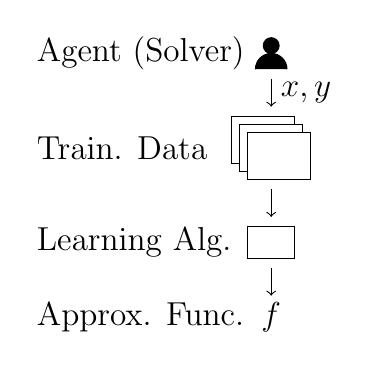
\begin{tikzpicture}
  \draw[fill=black]  (-2.8,3.7) ellipse (0.1 and 0.1);
  \draw[fill=black]  (-2.6,3.4) arc (0:180:0.2);
  \node[right] at (-5.9,3.6) {\large Agent (Solver)};
  \draw[fill=white]  (-3.3,2.8) rectangle (-2.5,2.2);
  \draw[fill=white]  (-3.2,2.7) rectangle (-2.4,2.1);
  \draw[fill=white]  (-3.1,2.6) rectangle (-2.3,2);
  \node[right] at (-5.9,2.4) {\large Train. Data};
  \node (v1) at (-2.8,3.4) {};
  \node (v2) at (-2.8,2.8) {};
  \draw[->]  (v1) edge (v2);
  \node[right] at (-2.8,3.1) {\large $x, y$};
  \node (v3) at (-2.8,2) {};
  \node (v4) at (-2.8,1.4) {};
  \draw[->]  (v3) edge (v4);
  \draw  (-3.1,1.4) rectangle (-2.5,1);
  \draw  (-2.4,3.2) rectangle (-2.4,3.2);
  \node[right] at (-5.9,1.2) {\large Learning Alg.};
  \node (v5) at (-2.8,1) {};
  \node (v6) at (-2.8,0.4) {};
  \draw[->]  (v5) edge (v6);
  \node[right] at (-5.9,0.25) {\large Approx. Func.};
  \node at (-2.8,0.25) {\large $f$};
  \end{tikzpicture}
  }
  \caption{Passive}
  \label{fig:passive}
  \end{subfigure}
  &
  \begin{subfigure}[b]{0.35\textwidth}
  \centering
  \resizebox{!}{2.75cm}{
  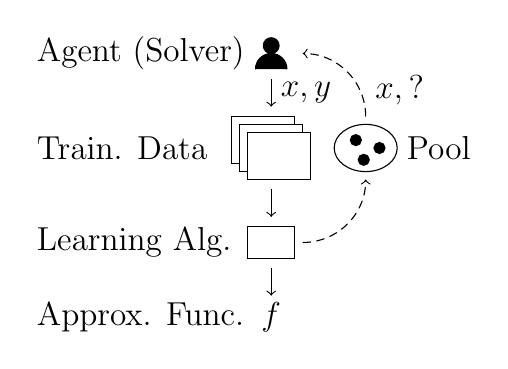
\begin{tikzpicture}
  \draw[fill=black]  (-2.8,3.7) ellipse (0.1 and 0.1);
  \draw[fill=black]  (-2.6,3.4) arc (0:180:0.2);
  \node[right] at (-5.9,3.6) {\large Agent (Solver)};
  \draw[fill=white]  (-3.3,2.8) rectangle (-2.5,2.2);
  \draw[fill=white]  (-3.2,2.7) rectangle (-2.4,2.1);
  \draw[fill=white]  (-3.1,2.6) rectangle (-2.3,2);
  \node[right] at (-5.9,2.4) {\large Train. Data};
  \node (v1) at (-2.8,3.4) {};
  \node (v2) at (-2.8,2.8) {};
  \draw[->]  (v1) edge (v2);
  \node[right] at (-2.8,3.1) {\large $x, y$};
  \node (v3) at (-2.8,2) {};
  \node (v4) at (-2.8,1.4) {};
  \draw[->]  (v3) edge (v4);
  \draw  (-3.1,1.4) rectangle (-2.5,1);
  \draw  (-2.4,3.2) rectangle (-2.4,3.2);
  \node[right] at (-5.9,1.2) {\large Learning Alg.};
  \node (v5) at (-2.8,1) {};
  \node (v6) at (-2.8,0.4) {};
  \draw[->]  (v5) edge (v6);
  \node[right] at (-5.9,0.25) {\large Approx. Func.};
  \node at (-2.8,0.25) {\large $f$};
  \node[right] at (-1.2,2.4) {\large Pool};
  \draw[->, densely dashed] (-2.4,1.2) arc (-90:0:0.8);
  \draw[->, densely dashed] (-1.6,2.8) arc (0:90:0.8);
  \node[right] at (-1.6,3.135) {\large $x, ?$};
  \draw  (-1.6,2.4) ellipse (0.4 and 0.3);
  \draw[fill=black]  (-1.725,2.5) ellipse (0.07 and 0.07);
  \draw[fill=black]  (-1.625,2.25) ellipse (0.07 and 0.07);
  \draw[fill=black]  (-1.425,2.4) ellipse (0.07 and 0.07);
  \end{tikzpicture}
  }
  \caption{Active Pool-based}
  \label{fig:activepool}
  \end{subfigure}
  &
  \begin{subfigure}[b]{0.35\textwidth}
  \centering
  \resizebox{!}{2.75cm}{
  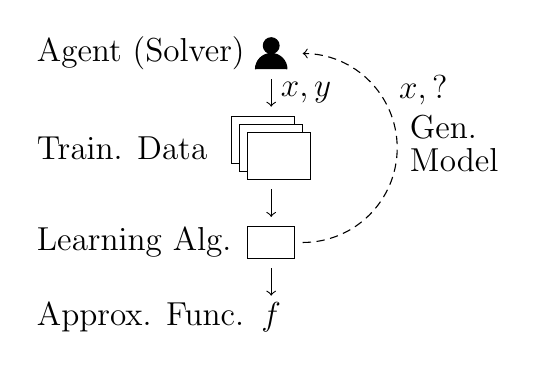
\begin{tikzpicture}
  \draw[fill=black]  (-2.8,3.7) ellipse (0.1 and 0.1);
  \draw[fill=black]  (-2.6,3.4) arc (0:180:0.2);
  \node[right] at (-5.9,3.6) {\large Agent (Solver)};
  \draw[fill=white]  (-3.3,2.8) rectangle (-2.5,2.2);
  \draw[fill=white]  (-3.2,2.7) rectangle (-2.4,2.1);
  \draw[fill=white]  (-3.1,2.6) rectangle (-2.3,2);
  \node[right] at (-5.9,2.4) {\large Train. Data};
  \node (v1) at (-2.8,3.4) {};
  \node (v2) at (-2.8,2.8) {};
  \draw[->]  (v1) edge (v2);
  \node[right] at (-2.8,3.1) {\large $x, y$};
  \node (v3) at (-2.8,2) {};
  \node (v4) at (-2.8,1.4) {};
  \draw[->]  (v3) edge (v4);
  \draw  (-3.1,1.4) rectangle (-2.5,1);
  \draw  (-2.4,3.2) rectangle (-2.4,3.2);
  \node[right] at (-5.9,1.2) {\large Learning Alg.};
  \node (v5) at (-2.8,1) {};
  \node (v6) at (-2.8,0.4) {};
  \draw[->]  (v5) edge (v6);
  \node[right] at (-5.9,0.25) {\large Approx. Func.};
  \node at (-2.8,0.25) {\large $f$};
  \node[right, label={[align=left]\large Gen.\\\large Model}] at (-0.6,1.85) {};
  %JB: does the model need to be a GAN or can it also be a different type of model?
  %TF: not necessarily, changed it
  \node[right] at (-1.3,3.135) {\large $x, ?$};
  \draw[->, densely dashed] (-2.4,1.2) arc (-90:90:1.2);
  \end{tikzpicture}
  }
  \caption{Active Synthesis-based}
  \label{fig:activesynth}
  \end{subfigure}
  \end{tabular}
  
  \caption{Types of Learning (depiction inspired by Rubens~et.al.~\cite{RubensESK15})}
  %JB: slightly larger font size in the figure (at least having the size of the caption) would be nice
  %TF: made it larger
  \label{fig:learning}
\end{figure}  

% Starting with only unlabeled data, e.g., a new user has not yet rated any content, an active-learning algorithm iteratively shows the items that are best suited to refine the user's model based on his previous interaction.
% In contrast to traditional passive machine-learning methods (Fig.~\ref{fig:passive}), active-learning approaches can actively select for which items to acquire labels~\cite{RubensESK15}.
% Since the potential runtime of experiments is by magnitudes larger than the model's training time, we only consider incrementing our benchmark set by one instance at a time rather than using batches which is also proposed in current active-learning advances~\cite{SinhaED19,TranDRC19}.

AL algorithms can be categorized into \emph{synthesis-bas\-ed} \cite{0001AEMN22,GarzonMG22,2019gaal} and \emph{pool-bas\-ed} approaches \cite{GolbandiKL11,HarpaleY08,KorenBV09}.%SinhaED19,distribAL,TongK01,KapoorGUD07,KornerW06,MelvilleM04}.
%JB: we can probably cut some citations, the three most important should be sufficient
%TF: done
While synthesis-based methods (Fig. \ref{fig:activesynth}) generate instances that might be interesting to label, pool-based methods (Fig. \ref{fig:activepool}) rely on a pool of unlabeled instances from which to draw items.

Recent synthesis-based methods within the field of satisfiability solving~\cite{0001AEMN22,GarzonMG22} show how to generate problem instances with desired properties.
This goal is, however, orthogonal to ours.
While those approaches want to generate problem instances on which a solver is good or bad, we want to predict whether a solver is good or bad on an existing benchmark set.

Pool-based methods can be further refined into \emph{Error-based} \cite{GolbandiKL11,KorenBV09}, \emph{Un\-cer\-tain\-ty-based} \cite{HarpaleY08,KapoorGUD07,TongK01}, \emph{Distribution-based} methods \cite{distribAL,SinhaED19} and \emph{Ensembles} \cite{KornerW06,MelvilleM04}.
Error-based strategies pick instances that have the most influence on the model parameters.
Uncertainty-based methods sample instances close to their perceived decision boundary.
Distribution-based approaches sample instances whose features are unaccounted for amongst the already sampled instances.
Finally, ensembles are a meta-strategy that combines the predictions of several different active-learning models into a selection choice.

In the field of SAT-solving, Volpato and Guangyan~\cite{volpato2019active} use uncertainty-sampling-based AL to learn an instance-specific algorithm selector.
Rather than benchmarking a solver's overall performance, the goal is to recommend the best solver out of a set of solvers for each SAT instance.

\subsubsection{Summary.}
To sum up this section, we have shown both traditional and recent benchmark-set-selection approaches.
Moreover, we have briefly outlined how active-learning techniques can help to incrementally select benchmark sets.
In the following sections, we present an active-learning-based benchmark-set-selection approach that solves the \emph{New-Solver Problem} while optimizing for runtime and fulfilling both comparability and scalability.

\section{Active Learning for SAT solver Benchmarking}
\label{sec:main}
Our framework follows a simple three-step schema (Alg.~\ref{algALBenchmark}).
%JB: as the algorithm is rather simple and has different parts to be plugged in, I think we should rebrand it as "framework" rather than algorithm (and change the term consistently in text)
%TF: changed
After initializing the model $\mathcal{M}$, we incrementally \emph{select} a problem instance from the pool of instances, one at a time, evaluate the new solver $\hat{a}$ on it, and \emph{update} the model with the acquired result.
We \emph{stop} when meeting some stopping condition.
Since the potential runtime of experiments is by magnitudes larger than the model's update time, we only consider incrementing our benchmark set by one instance at a time rather than using batches.
% For now, we also restrict ourselves to the aforementioned sequential one-instance-at-a-time process.
At the core of the model $\mathcal{M}$ is a prediction function $f\!: \left(\mathcal{A} \cup \left\lbrace \hat{a} \right\rbrace\right) \times \mathcal{I} \rightarrow \mathbb{R}$ that powers the decisions within the previously mentioned three steps.
%Note that the prediction target values may be also a subset of $\mathbb{R}$.
%Refer to the next sections for more details.

\begin{algorithm}
  \caption{Incremental benchmarking framework}
  \label{algALBenchmark}

  \KwIn{A pool of instances $\mathcal{I}$, a set of known solvers $\mathcal{A}$ with known runtimes $r\!: \mathcal{A} \times \mathcal{I} \rightarrow \left[0, \tau\right] \cup \left\lbrace \perp \right\rbrace$, and a new solver $\hat{a} \notin \mathcal{A}$.}

  $\mathcal{M} \leftarrow \textrm{init model with $\mathcal{A}$, $\mathcal{I}$, $r$, and $\hat{a}$}$
  
  $\tilde{\mathcal{I}} \leftarrow \emptyset$

  \While{$\operatorname{not} \, \operatorname{stop}\!\left(\mathcal{M}\right)$}{
    $s \leftarrow \operatorname{selectNextInstance}\!\left(\mathcal{M}\right)$

    $t \leftarrow \operatorname{runExperiment}\!\left(\hat{a},\,  s\right)$  \tcp*{Runs $\hat{a}$ on $s$ with time-out $\tau$}

    $\tilde{\mathcal{I}} \leftarrow \tilde{\mathcal{I}} \cup \left\lbrace s \right\rbrace$

    $\operatorname{updateModel}\!\left(\mathcal{M},\, s,\, t\right)$
  }

  $\operatorname{score}\!\left(\right) \leftarrow \operatorname{predictScores}\!\left(\mathcal{M}\right)$
  %JB: bit confusing that this is not a numerical score, but a function (see next line); maybe call it "score()"? or return a tuple with all estimated scores (one per solver?); also, one could expect to get a benchmark set as result (see title of algorithm), but since instance selection is solver-specific, this is not case (it's rather a benchmarking schema)
  %TF: renamed it to benchmarking framework and score()

  \KwOut{Return tuple of scoring function $\operatorname{score}\!: \mathcal{A} \cup \left\lbrace \hat{a} \right\rbrace \rightarrow \mathbb{R}$ and the selected instances $\tilde{\mathcal{I}}$.}
  %JB: we should formally specify the tuple rather than only describing it in words
  %TF: made it clearer
\end{algorithm}

The following section (Sec.~\ref{sec:main1}) discusses how we may derive a solver ranking from our model (line~8).
Thereafter, we look at possible sampling criteria (line~4) in Sec.~\ref{sec:main2} and, finally, possible stopping conditions (line~3) in Sec.~\ref{sec:main3}.

\subsection{Predicting Rankings}
\label{sec:main1}
In order to predict a ranking of solver $\hat{a}$ amidst its competitors, we need to infer its performance on all instances, even the ones on which we have not evaluated it.
To do so, there are generally two notions of this problem, i.e., regression and classification.
A regression model tries to predict the \mbox{PAR-2} runtime of $\hat{a}$ on all instances based on the samples that have been selected.
Then, the ranking is induced by the average predictions.
Alternatively, a classification model can be used to predict some discrete runtime labels of $\hat{a}$ on all instances.
Similarly, the average runtime label determines the ranking.

Preliminary experiments, as well as research in portfolio solvers~\cite{NgokoCT19,CollauttiMMO13}, have shown however that directly predicting runtimes without any transformation does not work well in practice.
%JB: Collauti at el. still predict actual (though normalized) runtimes rather than discrete labels, they only heavily discretize runtimes when using them as features
%TF: added "without any transformation"
%In our experiments, the mean squared error was within the same magnitude as the values to be predicted.
In contrast to that, discretizing runtimes and using those labels in the model's training and prediction yields good results (cf.~Sec.~\ref{sec:eval}).
The following paragraphs motivate why it makes sense to discretize runtimes.
%JB: we should probably cut this a bit
%TF: I've commented out a few sentences but we probably need to cut more.

We use a function $\gamma\!: {\mathcal{A} \times \mathcal{I}} \rightarrow \left\lbrace 1, \dots, k \right\rbrace$ to transform runtime observations.
In our experiments, this function is a clustering algorithm.
Note that this transformation is done per instance to adapt to different instance difficulties. 
Also, we define ${\gamma\!\left(a, i\right) := k}$ iff $r\!\left(a, i\right) = \,\perp$ for all $a \in \mathcal{A}$ and $i \in \mathcal{I}$.
To determine a ranking based on those labels, we define
\begin{equation}
  \operatorname{score}\!\left(a\right) := \frac{1}{|\mathcal{I}|} \sum_{i \in \mathcal{I}} w_{a,i} \cdot \left(\gamma\!\left(a, i\right) - 1\right) \enspace \textrm{,}
  %JB: does the "-1" provide any benefits, or does it only shift scores?
  %TF: it is used to resemble the 0-indexed implementation. I'm also not happy with this, but using \lbrace 0, \dots, k - 1 \rbrace does also look ugly.
  \label{eq:rankingeq}
\end{equation}
with $w_{a,i} := 2$ (PAR-\emph{2} penalty factor) if $\gamma\!\left(a, i\right) = k$ else $w_{a,i} := 1$.
To be applicable to $\hat{a}$, we extend \emph{score} by replacing $\gamma\!\left(a, i\right)$ by the model's predictions $f\!: \left(\mathcal{A} \cup \left\lbrace \hat{a} \right\rbrace\right) \times \mathcal{I} \rightarrow \left\lbrace 1, \dots, k \right\rbrace$.
%JB: as "$\operatorname{score}$" is not visibly different to the rest of the text, we should use some other way of highlighting
%TF: replaced it with emph{score} for now

Turning a regression into a classification problem, discretization is a useful tool.
However, it does not provide much value if the resulting cluster labels are not predictive of the PAR-2 ranking we seek to predict.
In our work, we use a hierarchical-clustering approach with a single-link criterion for $k = 3$.
For the SAT Competition~2022 Anniversary Track instances~\cite{sat2022}, this ranking approach is capable of correctly deciding for almost all pairs of solvers which one is faster (about \SI{97.45}{\%}; $\sigma = \SI{3.68}{\%}$).
Moreover, it decides all solvers correctly if the difference in the cluster-label-ranking scores between two solvers is at least \SI{0.11}{}.
%Refer to Table~\ref{tab:discreteranking} for a comparison with the PAR-2 ranking.
The Spearman correlation~\cite{de2016comparing} of cluster-label and PAR-2 ranking is about \SI{0.988} (in comparison to a perfect value of \SI{1}).
This shows that monotonicity and score distances between ranks align quite well between both ranking methods.

% In that sense, we also experiment with a combination of runtime-label ranking and the PAR-2 ranking of the subsample if the difference in label ranking scores drops below a certain threshold.
% Besides that, we additionally consider using the past $l$ model predictions in a voting approach for stability.

%\begin{table}[tbp]
%  \centering
%   \caption{
%     PAR-2 ranking vs. discretized-runtime ranking for the SAT Competition~2022 Anniversary Track instances~\cite{sat2022} ($k = 3$; hierarchical clustering).
%	  Differences are highlighted with a gray background.
%	}
%  \label{tab:discreteranking}
%  \begin{tabular}{
%    c
%    >{\centering\arraybackslash}p{1.8cm}p{3.6cm}
%    >{\centering\arraybackslash}p{1.8cm}p{3.6cm}
%  }
%    \hline
%    Rank & \multicolumn{2}{c}{PAR-2 Ranking} & \multicolumn{2}{c}{Cluster-Label Ranking} \\
%    \hline
%1   & 2806.400 & Kissat\_MAB\_ESA           & 1.172 & Kissat\_MAB\_ESA \\
%2   & 2810.959 & kissat-sc2022-bulky        & 1.183 & kissat-sc2022-bulky \\
%3   & 2830.143 & ekissat-mab-gb-db          & 1.185 & ekissat-mab-gb-db \\
%\cellcolor{gray!15} 4   & \cellcolor{gray!15} 2833.081 & \cellcolor{gray!15} Kissat\_MAB\_UCB           & \cellcolor{gray!15} 1.186 & \cellcolor{gray!15} kissat\_inc \\
%\cellcolor{gray!15} 5   & \cellcolor{gray!15} 2833.397 & \cellcolor{gray!15} kissat\_inc                & \cellcolor{gray!15} 1.186 & \cellcolor{gray!15} Kissat\_MAB\_UCB \\
%6   & 2841.734 & ekissat-mab-db-v1          & 1.192 & ekissat-mab-db-v1 \\
%7   & 2842.666 & Kissat\_MAB\_MOSS          & 1.192 & Kissat\_MAB\_MOSS \\
%8   & 2857.219 & Kissat\_MAB-HyWalk         & 1.195 & Kissat\_MAB-HyWalk \\
%9   & 2866.960 & kissat-sc2022-light        & 1.120 & kissat-sc2022-light \\
%10  & 2896.371 & kissat-els-v2              & 1.216 & kissat-els-v2 \\
%11  & 2950.179 & hKis-unsat                 & 1.229 & hKis-unsat \\
%12  & 2964.729 & Kissat\_adaptive\_restart  & 1.234 & Kissat\_adaptive\_restart \\
%13  & 2974.990 & SeqFROST-NoExtend          & 1.247 & SeqFROST-NoExtend \\
%14  & 3010.642 & Cadical\_ESA               & 1.248 & Cadical\_ESA \\
%\cellcolor{gray!15} 15  & \cellcolor{gray!15} 3012.152 & \cellcolor{gray!15} kissat-els-v1              & \cellcolor{gray!15} 1.258 & \cellcolor{gray!15} CadicalReorder \\
%\cellcolor{gray!15} 16  & \cellcolor{gray!15} 3028.922 & \cellcolor{gray!15} CadicalReorder             & \cellcolor{gray!15} 1.264 & \cellcolor{gray!15} kissat-els-v1 \\
%\cellcolor{gray!15} 17  & \cellcolor{gray!15} 3042.540 & \cellcolor{gray!15} cadical\_rel\_Scavel       & \cellcolor{gray!15} 1.278 & \cellcolor{gray!15} CaDiCaL\_DVDL\_V1 \\
%\cellcolor{gray!15} 18  & \cellcolor{gray!15} 3082.293 & \cellcolor{gray!15} kissat\_relaxed            & \cellcolor{gray!15} 1.283 & \cellcolor{gray!15} CaDiCaL\_DVDL\_V2 \\
%\cellcolor{gray!15} 19  & \cellcolor{gray!15} 3089.304 & \cellcolor{gray!15} CaDiCaL\_DVDL\_V1          & \cellcolor{gray!15} 1.298 & \cellcolor{gray!15} kissat\_relaxed \\
%\cellcolor{gray!15} 20  & \cellcolor{gray!15} 3095.118 & \cellcolor{gray!15} CaDiCaL\_DVDL\_V2          & \cellcolor{gray!15} 1.361 & \cellcolor{gray!15} cadical\_rel\_Scavel \\
%21  & 3272.674 & glucose-reboot             & 1.379 & glucose-reboot \\
%\cellcolor{gray!15} 22  & \cellcolor{gray!15} 3287.322 & \cellcolor{gray!15} LStech-Maple-HyWalk        & \cellcolor{gray!15} 1.414 & \cellcolor{gray!15} hCaD\_V1-psids \\
%23  & 3288.798 & LSTech\_Maple              & 1.446 & LSTech\_Maple \\
%\cellcolor{gray!15} 24  & \cellcolor{gray!15} 3399.281 & \cellcolor{gray!15} SLIME-SC-2022-beta         & \cellcolor{gray!15} 1.469 & \cellcolor{gray!15} LStech-Maple-HyWalk \\
%\cellcolor{gray!15} 25  & \cellcolor{gray!15} 3410.345 & \cellcolor{gray!15} SLIME-SC-2022              & \cellcolor{gray!15} 1.470 & \cellcolor{gray!15} SLIME-SC-2022-beta \\
%\cellcolor{gray!15} 26  & \cellcolor{gray!15} 3430.403 & \cellcolor{gray!15} hCaD\_V1-psids             & \cellcolor{gray!15} 1.523 & \cellcolor{gray!15} SLIME-SC-2022 \\
%27  & 3504.244 & MapleLCMDistChrBt-DL-v3    & 1.542 & MapleLCMDistChrBt-DL-v3 \\
%28  & 4750.808 & IsaSAT                     & 2.062 & IsaSAT \\
%    \hline
%  \end{tabular}
%\end{table}

That discretized runtimes are sufficient for distinguishing solvers can also be shown by comparing the fraction of solver pairs whose runtimes are significantly different.
Within the SAT~Competition~2022 Anniversary Track, about \SI{89.95}{\%} of solver pairs are significantly different (according to a Wilcoxon-signed-rank test with $\alpha = 0.05$).
While only time-out labels (solver times out or not on a particular instance) are sufficient to significantly distinguish about \SI{87.04}{\%} of solver pairs, discrete-runtime labels are sufficient to distinguish about \SI{87.83}{\%} of solver pairs.
%\footnote{Based on hierarchical clustering with a log-single-link criterion for $k = 3$.}
This means that we do not lose much discriminatory power using discrete runtime labels.
%The number of significant comparisons between solvers \emph{alone}, though, does only offer limited insights as we might achieve significant differences in all pairs by assigning some randomly skewed values as labels.
%JB: thus, we should reorder this section to mention the argument "significant difference" (this paragraph) first and "deciding solver pairs" (previous paragraph, stronger argument) second (rather than giving the stronger argument first, making the second argument superfluous)
%TF: Removed the previous sentence
The predictiveness of the PAR-2 score, the labels' discriminatory power, as well as that it enables us to use classification, show the clear advantage of runtime discretization.
%JB: at the same time with what? with the other benefits?
%TF: removed redundant phrase


\subsection{Instance Sampling}
\label{sec:main2}
Our instance-sampling strategies (also refer to Alg.~\ref{algALBenchmark}; line 4) can be divided into two categories.
First, we present possible baseline approaches including existing work on instance-based selection strategies~\cite{Bossek021a,GentHJKMNN14,MatriconAFSH21}.
%JB: approaches under "Second" are also at least "inspired by existing work" and probably also pick "interesting" instances, so distinction between the two categories of approaches not entirely clear
%TF: made it clearer. First = instance-based methods, second = model-based methods
Second, we show promising machine-learning-based sampling strategies that make use of the model's label-prediction function $f$ and are inspired by existing work within the realms of active learning~\cite{settles2009active}.

\subsubsection{Baselines and existing approaches.}
\label{sec:sampling1}
Apart from obvious baseline instance-selection strategies, i.e., random sampling and neighborhood-aware sampling (randomly choosing among the instances with the highest amount of non-sampled $k$ neighbors), we also implement existing instance-selection strategies.

Bossek and Wagner~\cite{Bossek021a} introduce a custom ranking-score metric incorporating the number of \emph{good} pairs and \emph{bad} pairs.
%JB: some selection methods, like this one, are not mentioned later anymore (in particular, not in experimental design), so we don't need to describe them in detail (maybe mention them shortly if used in preliminary experiments, but turned out to be not useful)
%TF: I've cut the section down a bit
A good solver pair, regarding a particular instance, are solvers that perform according to their global ranking.
%So if solver $a$ is better than solver $b$ on instance $i$ and $a$ is also in total better than $b$, it is a \emph{good} solver pair on $i$.
Otherwise, it is a \emph{bad} pair.
Based on this classification, they assign a custom score to each instance.
By selecting instances with the highest score, they try to favor instances that are predictive of the final ranking.
%This assumes, though, that the new solver $\hat{a}$ behaves similarly to the existing solvers.

Gent~et.~al.~\cite{GentHJKMNN14} make use of a concept known from racing for automated model selection.
Given a particular instance and a parameter $\rho$, a solver is $\rho$-dominated if it is at least $\rho$ times worse than the best solver on this problem instance.
By selecting instances with the highest amount of $\rho$-dominated solvers, they hope to sample instances that provide the best discriminatory power to distinguish the runtimes of a new contestant.

Finally, we also implement some of the selection approaches described by Matricon~et.al.~\cite{MatriconAFSH21}.
Besides uniformly random sampling and the aforementioned discrimination-based method by Gent~et.~al.~\cite{GentHJKMNN14}, they also describe a variance-based selection approach.
The variance-based strategy selects instances with the highest runtime variance per average runtime.
We also implement a logarithmized version of this, i.e., the highest log-runtime variance per average log runtime.
 
\subsubsection{Active-learning-based instance selection.}
\label{sec:sampling2}
For conciseness, we only present two of our active-learning-based instance-selection approaches, which show the most promising results.
We implement a model-uncertainty-based approach and a model-based information-gain sampling strategy.
%, and a voting-based committee-disagreement approach.

These methods require the model's predictions to also include probabilities for the $k$ possible runtime labels, i.e., 
\begin{equation}
  f'\!: \left(\mathcal{A} \cup \left\lbrace \hat{a} \right\rbrace\right) \times \mathcal{I} \rightarrow \left[0, 1\right]^k  \enspace \textrm{.}
\end{equation}
The model-uncertainty-based approach simply selects the instance that is closest to the model's decision boundary and, of course, not already selected, i.e.,
\begin{equation}
  \underset{i \in \mathcal{I} \setminus \tilde{\mathcal{I}}}{\arg\min} \left\lvert \frac{1}{k} - \max_{n \in \left\lbrace 1, \dots, k \right\rbrace} f'\!\left(\hat{a}, i\right)_{n} \right\rvert \enspace \textrm{.}
\end{equation}

The model-based information-gain sampling strategy selects the instance with the highest expected entropy reduction.
%This implicitly assumes that the model's runtime-label probabilities for an instance are close to being correct.
%JB: not sure what "close to being correct" means excactly: does strategy assume correct predictions, but implicitly has a tolerance for wrong predictions, or does it explicitly account for errors somehow?
%TF: removed the previous sentence as it probably confuses readers more and is not essential for the explanation
To be more specific, we select the instance $i$ that maximizes
\begin{equation}
  \operatorname{IG}\!\left(i\right) := \operatorname{H}\!\left(i\right) - \sum_{n = 1}^{k} f'\!\left(\hat{a}, i\right)_{n} \operatorname{H}\!\left(i, n\right) \enspace \textrm{,}
\end{equation}
whereby $\operatorname{H}\!\left(i\right)$ denotes the entropy of the runtime labels $\gamma\!\left(a, i\right)$ for all $a \in \mathcal{A}$ and $\operatorname{H}\!\left(i, n\right)$ denotes the entropy of the runtime labels including the runtime label of $\hat{a}$ which is $n$.
The term $\operatorname{H}\!\left(i, n\right)$ is computed for every possible runtime label $n$.

%Finally, the voting-based committee-disagreement approach requires a committee of $c$ models.
%Rather than having a single prediction function $f$, there is a separate function $f_j$ for all committee members $j \in \left\lbrace 1, \dots, c  \right\rbrace$.
%We then select the instance $i$ whose entropy of runtime-label votes by the different ensemble members is the highest.

\subsection{Stopping Criteria}
\label{sec:main3}
Similar to the instance-selection strategies, we can also divide stopping criteria into baseline and active-learning-based approaches.
Also, refer to~Alg.~\ref{algALBenchmark}, line~3.
While a fixed subset-size criterion, e.g., only sample \SI{20}{\%} of all available instances, is an example of the former, a stopping criterion based on a Wilcoxon signed-rank test or the convergence of the model's predictions is an example for the latter.

The Wilcoxon stopping criterion stops the iterative active-learning algorithm when we are on average certain enough that the predicted runtime labels are sufficiently different in comparison to the other solvers.
To be more specific, we stop when
\begin{equation}
  W_{\hat{a}} := \frac{1}{\left\lvert \mathcal{A} \right\rvert} \sum_{a \in \mathcal{A}} \operatorname{wilcoxon}_{\alpha}\!\left(\gamma\!\left(a, \mathcal{I}\right), f\!\left(\hat{a}, \mathcal{I}\right) \right)
\end{equation}
drops below a certain threshold.
%JB: if this is info gain regarding runtimes, doesn't Eq. (4) mean that we would prefer instances with low entropy of runtime distribution after considering the new solver, i.e., instances that are not very discriminatory?
%TF: I don't think so. We want to maximize the reduction in entropy of the runtime labels. Low entropy afterward -> we know that the solver behaves similarly to existing ones.
Thereby, \emph{wilcoxon} denotes the $p$-value of a Wilcoxon signed-rank test of the runtime-label distributions and $\gamma\!\left(a, \mathcal{I}\right)$ and $f\!\left(\hat{a}, \mathcal{I}\right)$ are the natural set extensions on $\gamma$ and $f$ respectively.
%JB: "set extension" might be rather technical and hard to understand; also, why "expected"? in the sense of "straightforward"?
%TF: I already saw this expression in other papers. I'm not sure how to say the same thing clearer in the same amount of space.
To improve the stability of this criterion, we use an exponential moving average
\begin{equation}
  W_{\exp}^{\left(m\right)} := \beta W_{\hat{a}} + \left(1 - \beta\right) W_{\exp}^{\left(m - 1\right)} \enspace \textrm{,}
\end{equation}
whereby $m$ denotes the count of iterations within Alg.~\ref{algALBenchmark} and $W_{\exp}^{\left(0\right)} := 1$.

The model-convergence stopping criterion is less sophisticated in comparison.
It simply stops the active-learning process (Alg.~\ref{algALBenchmark}) if within the last $l$ iterations the ranking that is induced by the model's predictions (Eq.~\ref{eq:rankingeq}) remains unchanged.
Note that the concrete values of $\operatorname{score}\!\left(a\right)$ might still change.
We are solemnly interested in the induced ranking in this case.


\section{Experimental Design}
Given all the previously presented instantiations for Alg.~\ref{algALBenchmark}, this section briefly outlines our experimental design, including our optimization goal, evaluation framework, used data sets, hyper-parameter choices, as well as implementation details.
% hyper-parameter values that we experiment with

\subsection{Optimization Goal}
\label{sec:goal}
As already stated in the introductory section, this work addresses the \emph{New-Solver Problem} (cf.~Def.~\ref{def:new-solver-problem}).
By running Alg.~\ref{algALBenchmark}, we obtain a prediction model $\mathcal{M}$ that provides us with a scoring function \emph{score}.
Also, it outputs the fraction of runtime that is needed to arrive at its conclusion.
First and foremost, our goal is to provide the engineer of new SAT solvers with an accurate ranking.
We define the \emph{ranking accuracy} $O_{\operatorname{acc}} \in \left[0, 1\right]$ (higher is better) by the fraction of pairs $\left(\hat{a}, a\right)$ for all $a \in \mathcal{A}$ that are decided correctly by the given ranking (cf. Alg.~\ref{alg:eval}).
For now, we exclude the equality of solvers since data shows that the PAR-2 scores of all our solvers are different.
So, possible ranking decisions may be, for example, solver $a$ is better than $b$ or $b$ is better than $a$.
The ranking accuracy is affected by whether this decision is correctly made.
Matricon et. al.~\cite{MatriconAFSH21} also evaluate their approach by the fraction of solver pairs that is correctly decided.
Second, we also have to optimize for runtime.
The \emph{fraction of runtime} that the algorithm needs to arrive at its conclusion is denoted by $O_{\operatorname{rt}} \in \left[0, 1\right]$ (lower is better).
This metric puts the runtime summed over the sampled instances in relation to the runtime summed over all instances in the dataset (cf. Alg.~\ref{alg:eval}).
Overall, we want to find an approach that maximizes
\begin{equation}
  O_\delta := \delta O_{\operatorname{acc}} + \left(1 - \delta\right) \left(1 - O_{\operatorname{rt}}\right) \enspace \textrm{,}
  \label{eq:opt}
\end{equation} 
whereby $\delta \in \left[0, 1\right]$ allows for linear weighting between the two optimization goals $O_{\operatorname{acc}}$ and $O_{\operatorname{rt}}$.
Plotting the approaches that maximize $O_\delta$ for all $\delta \in \left[0, 1\right]$ on a $O_{\operatorname{rt}}$-$O_{\operatorname{acc}}$-diagram provides us with a Pareto front of the best approaches for different optimization-goal weightings.

\subsection{Evaluation Framework}
\label{sec:evalframe}
To evaluate a concrete instantiation of Alg.~\ref{algALBenchmark} (a concrete choice for all the sub-routines), we perform cross-validation on our set of solvers.
That means that each solver once plays the role of the new solver.
Alg.~\ref{alg:eval} shows this.
Note that the \emph{new} solver in each iteration is excluded from the set of solvers $\mathcal{A}$ to avoid data leakage.
Also, the runtime function $r$ is restricted to $\mathcal{A} \times \mathcal{I}$.

\vspace{-0.2cm}
\begin{algorithm}[htbp]
  \caption{Evaluation framework}
  \label{alg:eval}

  \KwIn{A pool of instances $\mathcal{I}$, a set of solvers $\mathcal{S}$ with known runtimes $r\!: \mathcal{S} \times \mathcal{I} \rightarrow \left[0, \tau\right] \cup \left\lbrace \perp \right\rbrace$, and PAR-2 scores $par2\!: \mathcal{S} \rightarrow \mathbb{R}$ for each solver.}

  $res \leftarrow \emptyset$

  \For{$\hat{a} \in \mathcal{S}$}{
    $\mathcal{A} \leftarrow \mathcal{S} \setminus \left\lbrace \hat{a} \right\rbrace$

    $\left( score,\, \tilde{\mathcal{I}} \right) \leftarrow \operatorname{runALAlgorithm}\!\left(\mathcal{I}, \mathcal{A}, \left.r\right|_{\mathcal{A} \times \mathcal{I}}, \hat{a}\right)$ \tcp*{Refer to Alg.~\ref{algALBenchmark}}

    $O_{\operatorname{acc}} \leftarrow \left(\sum_{a \in \mathcal{A}} \left[\operatorname{sign}\!\left(score\!\left(a\right) - score\!\left(\hat{a}\right)\right) = \operatorname{sign}\!\left(par2\!\left(a\right) - par2\!\left(\hat{a}\right)\right) \right]\right) / |\mathcal{A}|$
    
    \tcp*{Iverson-bracket notation}

    $O_{\operatorname{rt}} \leftarrow \left(\sum_{i \in \tilde{\mathcal{I}}} r\!\left(i, \hat{a}\right)\right) / \left(\sum_{i \in \mathcal{I}} r\!\left(i, \hat{a}\right)\right)$
    %JB: do we need to call a function here or can't we directly write how this is computed (define a variable starting at 0 to which the runtime fraction is added each iteration)?
    %TF: fixed

    $res \leftarrow res \cup \left\lbrace \left( O_{\operatorname{acc}},\, O_{\operatorname{rt}} \right) \right\rbrace$
  }

  $\left( \bar{O}_{\operatorname{acc}},\, \bar{O}_{\operatorname{rt}} \right) \leftarrow \operatorname{mean}\!\left( res \right)$

  \KwOut{Return the average ranking accuracy $\bar{O}_{\operatorname{acc}}$ and the average fraction of runtime needed $\bar{O}_{\operatorname{rt}}$.}
\end{algorithm}
\vspace{-0.2cm}

\subsection{Data}
In our experiments, we work with the SAT~Competition~2022 Anniversary Track instances~\cite{sat2022}.
The dataset consists of 5355 instances with respective runtime data.
It has complete runtimes of 28 solvers.
We use the GBD metadata database~\cite{IserS18} to provide us with the aforementioned instance features, problem instances, and solver runtimes.
Thereby, all our approaches make use of the 56 base features that are maintained in the \emph{base} database of GBD~\cite{IserS18}.
They are inspired by the SATzilla features~\cite{features}.
Those features comprise general instance-size features and graph-representation features among others.
All features are numeric and fortunately free of any missing values.
We drop 10 out of 56 features because of zero variance.
For hyper-parameter tuning, we randomly sample \SI{10}{\%} of the complete set of 5355 instances with stratification regarding the instance's family.
All instance families that are too \emph{small}, i.e., \SI{10}{\%} of them corresponds to less than one instance, are put into one meta-family for stratification.
This smaller dataset allows for a more extensive exploration of hyper-parameter space.

\subsection{Hyper-parameters}
\label{sec:hyper}
Given Alg.~\ref{algALBenchmark}, there are several possible instantiations for the three phases, i.e., \emph{selection}, \emph{stopping}, and \emph{ranking}.
Also, there are different choices for the runtime-label prediction model.
Note that we are not considering all previously listed approaches since a grid search of all combinations would be infeasible.
Rather, we filter approaches based on preliminary experimental results (cf. Sec.~\ref{sec:evalprel}) and do the main end-to-end experiments only with a subset.
The end-to-end experiment configurations are given below.
%JB: still interesting to see which approaches were considered in preliminary experiments; could also list them here and indicate somehow which methods were only used preliminarily (e.g., by putting "(preliminary experiments only)" or some shorter label/sign behind them)
%TF: Added some selection methods that are mentioned.

\subsubsection{Ranking.}
Regarding \emph{ranking} (cf. Sec.~\ref{sec:main1}), we experiment with the following approaches, including our used hyper-parameter values:
%JB: as parts of these approaches are mostly new to readers (Section 3.1 only explains prediction-based ranking in general, neither observed ranking nor history nor fallback), I'm not sure if we should provide further motivation/explanation here); also applies to other components of experimental design
%TF: I've tried to add some more information. 
\begin{itemize}
  \item Observed PAR-2 ranking of already sampled instances
  \item Predicted ranking induced by runtime-label predictions
  \begin{itemize}
    \item History size: consider the latest 1, 10, 20, 30, or 40 predictions within a voting approach for stability. Given a particular ranking decision, the latest $x$ predictions vote on the winner.
    \item Fallback threshold: if the difference of scores between two solvers drops below \SI{0.01}, \SI{0.05}, or \SI{0.1}, use the partially observed PAR-2 ranking as a tie-breaker. As discussed in Sec.~\ref{sec:main1}, ranking decisions are all correct if the difference in scores between two solvers exceeds a certain value.
    %JB: "difference of ranking" between a pair of new solver and another solver? or has this phrase a different meaning?
    %TF: tried to clarify
  \end{itemize}
\end{itemize}

\subsubsection{Selection.}
For \emph{selection} (cf. Sec.~\ref{sec:sampling1}), we experiment with the following methods, including our used hyper-parameter values:
%JB: the referenced sampling section describes more methods than the ones listed below, so I guess some methods got dropped after preliminary experiments
%TF: added them
\begin{itemize}
  \item Random sampling 
  \item Model-based uncertainty sampling
  \begin{itemize}
    \item Fallback threshold: use random sampling for the first \SI{0}{\%}, \SI{5}{\%}, \SI{10}{\%}, \SI{15}{\%}, or \SI{20}{\%} of instances to explore the instance space.
    \item Runtime scaling: prefer instances with the greatest uncertainty per average runtime (\texttt{True} or \texttt{False}).
    %JB: how does this scaling work exactly? divide runtimes by average runtime of all solvers on that instance?
    %TF: yes
  \end{itemize}

  \item Model-based information-gain sampling
  \begin{itemize}
    \item Fallback threshold: use random sampling for the first \SI{0}{\%}, \SI{5}{\%}, \SI{10}{\%}, \SI{15}{\%}, or \SI{20}{\%} of instances to explore the instance space.
    \item Runtime scaling: prefer instances with the greatest information-gain per average runtime (\texttt{True} or \texttt{False}).
  \end{itemize}

  \item Neighborhood-aware random sampling (preliminary experiments only); randomly chooses among the instances with the highest amount of non-sampled $k$ neighbors
  \item Ranking-based sampling~\cite{Bossek021a} (preliminary experiments only)
  \item Discrimination-based sampling~\cite{GentHJKMNN14} (preliminary experiments only)
  \item Variance-based sampling~\cite{MatriconAFSH21} (preliminary experiments only)
\end{itemize}

\subsubsection{Stopping.}
For \emph{stopping} decisions (cf. Sec.~\ref{sec:main3}), we experiment with the following criteria, including our used hyper-parameter values:
\begin{itemize}
  \item Fixed subset size of \SI{10}{\%} or \SI{20}{\%} of instances
  \item Ranking convergence criterion
  \begin{itemize}
    \item Minimum amount: sample at least \SI{2}{\%}, \SI{8}{\%}, \SI{10}{\%}, or \SI{12}{\%} of instances before applying the criterion.
    \item Convergence duration: stop if the predicted ranking stays the same for the last \SI{1}{\%} or \SI{2}{\%} of sampled instances.
    %JB: why this fraction and not an absolute number of instances? the definition here might make stopping in early iterations rather likely, as just very few consecutive instances are needed (which might happen by coincidence; e.g., for ~5k instances, 2% minimum amount-> ~100 instances, 1% convergence duration -> ~1 instance), while the criterion becomes harder in later iterations
    %TF: for that reason, it is combined with the "minimum amount". Using fractions makes the approach more useful when adapting it to benchmarks of different sizes.
  \end{itemize}

  \item Wilcoxon criterion
  \begin{itemize}
    \item Minimum amount: sample at least \SI{2}{\%}, \SI{8}{\%}, \SI{10}{\%}, or \SI{12}{\%} of instances before applying the criterion.
    \item Average of $p$-values to drop below: \SI{5}{\%}.
    \item Exponential-moving average: incorporate previous significance values by using an EMA with $\beta = 0.1$ or $\beta = 0.7$.
  \end{itemize}
\end{itemize}

\subsubsection{Runtime-label prediction model.}
As a runtime-label prediction model, we only make use of one method that has proven to be successful in preliminary experiments (cf.~Sec.~\ref{sec:evalprel}).
Our model of choice is an ensemble, stacking a quadratic-discriminant analysis\footnote{With a regularization parameter of zero and a singular value threshold of zero} onto a random forest model\footnote{With \emph{entropy} splitting criterion and \emph{balanced} class weights} using a decision tree\footnote{With \emph{Gini} impurity splitting criterion; choosing the best split for each branching decision and maximum tree depth of 5 levels} to weight its members.
If not stated explicitly, all other model parameters default to the presets of \emph{scikit-learn}\footnote{\url{https://scikit-learn.org/stable/index.html}; Version 1.0.2}~\cite{scikit-learn}.

%the proposed runtime label ranking, (2) the PAR-2 subsample ranking, and (3) the runtime label ranking that uses the PAR-2 subsample ranking as a fallback when performance differences drop below a threshold.
%Possible values are \SI{0.01}{}, \SI{0.05}{}, and \SI{0.1}{}.
%Also, we experiment with different lengths of the prediction history that is used for stabilizing the ranking.
%Possible values are 10, 20, 30, 40, and 50.

\subsection{Implementation Details}
For reproducibility, our source code, all experiments, and data are available on GitHub\footnote{\url{https://github.com/mathefuchs/al-for-SAT solver-benchmarking}}.
Our code is implemented in \textsc{Python} using \emph{scikit-learn}~\cite{scikit-learn} for making predictions and \emph{gbd-tools}~\cite{IserS18} for SAT-instance retrieval.


\section{Evaluation}
\label{sec:eval}
Now that we are all set, we want to, first, discuss preliminary results including the choice of the runtime-discretization method and the choice of the machine-learning predictor.
Thereafter, we look at end-to-end results and instance-family importance.
%JB: instance families not really motivated till now, only appear in abstract and in text regarding stratification

\subsection{Preliminary Results}
\label{sec:evalprel}
%JB: if we dedicate a whole section to these results, we should probably rename this section (not "preliminary" in the typical sense); for TACAS, I guess this can be cut a bit
An exhaustive grid search of all approaches outlined in Sec.~\ref{sec:main} is infeasible.
We are, therefore, narrowing down the search by filtering based on preliminary results.
Since all relevant decisions, i.e., \emph{selection}, \emph{stopping}, and \emph{ranking}, revolve around the choice of prediction model, we are first looking at the \emph{Matthews Correlation Coefficient} (MCC) scores~\cite{gorodkin2004comparing,matthews1975comparison} that a particular prediction model achieves.
MCC scores are great in dealing with class imbalances in contrast to conventional metrics like accuracy.

\begin{table}
  \centering
  \caption{
  	Time-out prediction Matthews Correlation Coefficient performances.
  	Results are obtained using cross-validation.
  	We provide \SI{64}{\%} of ground-truth for training, use \SI{16}{\%} as a validation set, and \SI{20}{\%} as a test set (5-fold cross-validation).
  }
  \label{tab:mcc}
  \begin{tabular}{lc}
    Prediction Model & Avg. MCC (Std.) \\
    \hline
    Stacking ensemble (QDA, RF)           & 0.9527 (0.0292) \\
    Quadratic-discriminant analysis (QDA) & 0.9290 (0.0339) \\
    Random forest (RF)                    & 0.8530 (0.0479) \\
    AdaBoost with decision trees          & 0.8384 (0.0444) \\
    AdaBoost with logistic regression     & 0.8158 (0.0985) \\
    Decision tree                         & 0.8059 (0.0707) \\
    Logistic regression                   & 0.8052 (0.1018) \\
    kNN classifier                        & 0.7885 (0.1521) \\
    MLP classifier                        & 0.7760 (0.1408) \\
    Support-vector classifier             & 0.7757 (0.2149) \\
    Naive Bayes                           & 0.7306 (0.1394) \\
    \hline
  \end{tabular}
\end{table}

% Stacking MCC
% 0.888221577313471
% 0.04753979056930393

To obtain the results in Table~\ref{tab:mcc}, we perform cross-validation among all solvers: we assume that all other solver runtimes are known and provide \SI{64}{\%} of ground-truth runtime labels of the target solver for training, use \SI{16}{\%} as a validation set for hyper-parameter tuning, and \SI{20}{\%} as a test set (5-fold cross-validation).
This is repeated for each solver once.
Note that we perform cross-validation on two levels, i.e., among the solvers and the target solver runtimes.
We report the average performances on the test sets.
Since the differences in the MCC-performance distributions of the best and second-best approaches are statistically significant regarding a Wilcoxon signed-rank test with $\alpha = \SI{5}{\%}$, we only use the best approach for all further experiments as a prediction model.

As a runtime discretization technique, we use hierarchical clustering with $k = 3$ using a log-single-link criterion for all further experiments.
Each non-time-out runtime starts in a separate interval.
We then gradually merge intervals whose single-link logarithmic distance is the smallest until the desired number of partitions is reached.
As already mentioned in Sec.~\ref{sec:main1}, this approach has good properties regarding the predictiveness of the PAR-2 score ranking and its discriminatory power.
Also, preliminary experiments showed that our stacking ensemble performed particularly well for this kind of discretization method.
Other clustering approaches that we have tried include hierarchical clustering with mean-, median- and complete-link criteria, as well as $k$-means and spectral clustering.
Predicting runtime labels in a similar experiment as above produced an MCC score of on average \SI{88.82}{\%} ($\sigma = \SI{4.75}{\%}$; in comparison to \SI{95.27}{\%} for predicting time-outs).
%JB: "similar experiment as above" - reference unclear; what do you want to say?

\subsection{Experimental Results}
\subsubsection{Tuning our algorithm.}
Our main end-to-end experiments follow the evaluation framework that has been introduced in Sec.~\ref{sec:evalframe}.
Fig.~\ref{fig:e2eallsolvers} shows the performance of the approaches listed in Sec.~\ref{sec:hyper} on $O_{\operatorname{rt}}$-$O_{\operatorname{acc}}$-diagrams for the smaller hyper-parameter-tuning dataset.
The plotted lines represent the Pareto front for each possible choice of ranking approaches (Fig.~\ref{fig:annitraincolorranking}), selection approaches (Fig.~\ref{fig:annitraincolorselection}), and stopping criteria (Fig.~\ref{fig:annitraincolorstopping}).
%JB: as far as I understand it, the lines only compare some top-level hyperparameters, but for each of these hyperparemeters, take the best (= Pareto front) out of some more fine-grained settings (the hyperparameters of the hyperparameters, so to speak), so it's no really "each possible choice" in the sense of actual, individual configurations, but rather a combination of configurations
Colors indicate the different hyper-parameter instantiations.
To be more specific, they represent the Pareto front of all configurations with the respective instantiations.

Regarding the ranking approach (Fig.~\ref{fig:annitraincolorranking}), using the ranking that is induced by our runtime-label predictions consistently performs better than the partially observed PAR-2 ranking for each possible value of $\delta$.
%JB: as in previous comment: consistent outperformance not guaranteed in case the lines are not individual approaches, but Pareto fronts within the compared categories (which means that different parts of the line might be related to different hyperparameter settings)
%This was expected since a possible bias in the selection decisions of the model is accounted for when using the model's predictions for ranking.
This is expected since selection decisions are not random.
For example, we might sample more instances of one family if it benefits discrimination of solvers.
While the partially observed PAR-2 score is skewed, the prediction model can account for this.

Regarding the selection approaches (Fig.~\ref{fig:annitraincolorselection}), the model-based uncertainty strategy performs best in most cases.
However, the model-based information-gain sampling is beneficial if runtime is strongly favored (very small $\delta$; runtime fraction less than \SI{5}{\%}).
%JB: we should also describe performance of random sampling, which is visible in plot as well

Regarding the stopping criterion (Fig.~\ref{fig:annitraincolorstopping}), the ranking convergence criterion performs the most consistently well.
If PAR-2 accuracy is strongly favored (very high $\delta$), the Wilcoxon stopping criterion performs better.

\begin{figure}[tbp!]
  \centering
  \begin{subfigure}{1.0\textwidth}
    \resizebox{\textwidth}{!}{
      \graphicspath{{../plots/}}
      %% Creator: Matplotlib, PGF backend
%%
%% To include the figure in your LaTeX document, write
%%   \input{<filename>.pgf}
%%
%% Make sure the required packages are loaded in your preamble
%%   \usepackage{pgf}
%%
%% Also ensure that all the required font packages are loaded; for instance,
%% the lmodern package is sometimes necessary when using math font.
%%   \usepackage{lmodern}
%%
%% Figures using additional raster images can only be included by \input if
%% they are in the same directory as the main LaTeX file. For loading figures
%% from other directories you can use the `import` package
%%   \usepackage{import}
%%
%% and then include the figures with
%%   \import{<path to file>}{<filename>.pgf}
%%
%% Matplotlib used the following preamble
%%
\begingroup%
\makeatletter%
\begin{pgfpicture}%
\pgfpathrectangle{\pgfpointorigin}{\pgfqpoint{9.333576in}{3.346586in}}%
\pgfusepath{use as bounding box, clip}%
\begin{pgfscope}%
\pgfsetbuttcap%
\pgfsetmiterjoin%
\pgfsetlinewidth{0.000000pt}%
\definecolor{currentstroke}{rgb}{1.000000,1.000000,1.000000}%
\pgfsetstrokecolor{currentstroke}%
\pgfsetstrokeopacity{0.000000}%
\pgfsetdash{}{0pt}%
\pgfpathmoveto{\pgfqpoint{-0.000000in}{0.000000in}}%
\pgfpathlineto{\pgfqpoint{9.333576in}{0.000000in}}%
\pgfpathlineto{\pgfqpoint{9.333576in}{3.346586in}}%
\pgfpathlineto{\pgfqpoint{-0.000000in}{3.346586in}}%
\pgfpathlineto{\pgfqpoint{-0.000000in}{0.000000in}}%
\pgfpathclose%
\pgfusepath{}%
\end{pgfscope}%
\begin{pgfscope}%
\pgfsetbuttcap%
\pgfsetmiterjoin%
\definecolor{currentfill}{rgb}{1.000000,1.000000,1.000000}%
\pgfsetfillcolor{currentfill}%
\pgfsetlinewidth{0.000000pt}%
\definecolor{currentstroke}{rgb}{0.000000,0.000000,0.000000}%
\pgfsetstrokecolor{currentstroke}%
\pgfsetstrokeopacity{0.000000}%
\pgfsetdash{}{0pt}%
\pgfpathmoveto{\pgfqpoint{0.746177in}{0.679475in}}%
\pgfpathlineto{\pgfqpoint{9.093551in}{0.679475in}}%
\pgfpathlineto{\pgfqpoint{9.093551in}{3.163253in}}%
\pgfpathlineto{\pgfqpoint{0.746177in}{3.163253in}}%
\pgfpathlineto{\pgfqpoint{0.746177in}{0.679475in}}%
\pgfpathclose%
\pgfusepath{fill}%
\end{pgfscope}%
\begin{pgfscope}%
\pgfsetbuttcap%
\pgfsetroundjoin%
\definecolor{currentfill}{rgb}{0.000000,0.000000,0.000000}%
\pgfsetfillcolor{currentfill}%
\pgfsetlinewidth{0.803000pt}%
\definecolor{currentstroke}{rgb}{0.000000,0.000000,0.000000}%
\pgfsetstrokecolor{currentstroke}%
\pgfsetdash{}{0pt}%
\pgfsys@defobject{currentmarker}{\pgfqpoint{0.000000in}{-0.048611in}}{\pgfqpoint{0.000000in}{0.000000in}}{%
\pgfpathmoveto{\pgfqpoint{0.000000in}{0.000000in}}%
\pgfpathlineto{\pgfqpoint{0.000000in}{-0.048611in}}%
\pgfusepath{stroke,fill}%
}%
\begin{pgfscope}%
\pgfsys@transformshift{0.746177in}{0.679475in}%
\pgfsys@useobject{currentmarker}{}%
\end{pgfscope}%
\end{pgfscope}%
\begin{pgfscope}%
\definecolor{textcolor}{rgb}{0.000000,0.000000,0.000000}%
\pgfsetstrokecolor{textcolor}%
\pgfsetfillcolor{textcolor}%
\pgftext[x=0.746177in,y=0.582253in,,top]{\color{textcolor}\rmfamily\fontsize{18.000000}{21.600000}\selectfont 0.0}%
\end{pgfscope}%
\begin{pgfscope}%
\pgfsetbuttcap%
\pgfsetroundjoin%
\definecolor{currentfill}{rgb}{0.000000,0.000000,0.000000}%
\pgfsetfillcolor{currentfill}%
\pgfsetlinewidth{0.803000pt}%
\definecolor{currentstroke}{rgb}{0.000000,0.000000,0.000000}%
\pgfsetstrokecolor{currentstroke}%
\pgfsetdash{}{0pt}%
\pgfsys@defobject{currentmarker}{\pgfqpoint{0.000000in}{-0.048611in}}{\pgfqpoint{0.000000in}{0.000000in}}{%
\pgfpathmoveto{\pgfqpoint{0.000000in}{0.000000in}}%
\pgfpathlineto{\pgfqpoint{0.000000in}{-0.048611in}}%
\pgfusepath{stroke,fill}%
}%
\begin{pgfscope}%
\pgfsys@transformshift{1.580914in}{0.679475in}%
\pgfsys@useobject{currentmarker}{}%
\end{pgfscope}%
\end{pgfscope}%
\begin{pgfscope}%
\definecolor{textcolor}{rgb}{0.000000,0.000000,0.000000}%
\pgfsetstrokecolor{textcolor}%
\pgfsetfillcolor{textcolor}%
\pgftext[x=1.580914in,y=0.582253in,,top]{\color{textcolor}\rmfamily\fontsize{18.000000}{21.600000}\selectfont 0.1}%
\end{pgfscope}%
\begin{pgfscope}%
\pgfsetbuttcap%
\pgfsetroundjoin%
\definecolor{currentfill}{rgb}{0.000000,0.000000,0.000000}%
\pgfsetfillcolor{currentfill}%
\pgfsetlinewidth{0.803000pt}%
\definecolor{currentstroke}{rgb}{0.000000,0.000000,0.000000}%
\pgfsetstrokecolor{currentstroke}%
\pgfsetdash{}{0pt}%
\pgfsys@defobject{currentmarker}{\pgfqpoint{0.000000in}{-0.048611in}}{\pgfqpoint{0.000000in}{0.000000in}}{%
\pgfpathmoveto{\pgfqpoint{0.000000in}{0.000000in}}%
\pgfpathlineto{\pgfqpoint{0.000000in}{-0.048611in}}%
\pgfusepath{stroke,fill}%
}%
\begin{pgfscope}%
\pgfsys@transformshift{2.415652in}{0.679475in}%
\pgfsys@useobject{currentmarker}{}%
\end{pgfscope}%
\end{pgfscope}%
\begin{pgfscope}%
\definecolor{textcolor}{rgb}{0.000000,0.000000,0.000000}%
\pgfsetstrokecolor{textcolor}%
\pgfsetfillcolor{textcolor}%
\pgftext[x=2.415652in,y=0.582253in,,top]{\color{textcolor}\rmfamily\fontsize{18.000000}{21.600000}\selectfont 0.2}%
\end{pgfscope}%
\begin{pgfscope}%
\pgfsetbuttcap%
\pgfsetroundjoin%
\definecolor{currentfill}{rgb}{0.000000,0.000000,0.000000}%
\pgfsetfillcolor{currentfill}%
\pgfsetlinewidth{0.803000pt}%
\definecolor{currentstroke}{rgb}{0.000000,0.000000,0.000000}%
\pgfsetstrokecolor{currentstroke}%
\pgfsetdash{}{0pt}%
\pgfsys@defobject{currentmarker}{\pgfqpoint{0.000000in}{-0.048611in}}{\pgfqpoint{0.000000in}{0.000000in}}{%
\pgfpathmoveto{\pgfqpoint{0.000000in}{0.000000in}}%
\pgfpathlineto{\pgfqpoint{0.000000in}{-0.048611in}}%
\pgfusepath{stroke,fill}%
}%
\begin{pgfscope}%
\pgfsys@transformshift{3.250389in}{0.679475in}%
\pgfsys@useobject{currentmarker}{}%
\end{pgfscope}%
\end{pgfscope}%
\begin{pgfscope}%
\definecolor{textcolor}{rgb}{0.000000,0.000000,0.000000}%
\pgfsetstrokecolor{textcolor}%
\pgfsetfillcolor{textcolor}%
\pgftext[x=3.250389in,y=0.582253in,,top]{\color{textcolor}\rmfamily\fontsize{18.000000}{21.600000}\selectfont 0.3}%
\end{pgfscope}%
\begin{pgfscope}%
\pgfsetbuttcap%
\pgfsetroundjoin%
\definecolor{currentfill}{rgb}{0.000000,0.000000,0.000000}%
\pgfsetfillcolor{currentfill}%
\pgfsetlinewidth{0.803000pt}%
\definecolor{currentstroke}{rgb}{0.000000,0.000000,0.000000}%
\pgfsetstrokecolor{currentstroke}%
\pgfsetdash{}{0pt}%
\pgfsys@defobject{currentmarker}{\pgfqpoint{0.000000in}{-0.048611in}}{\pgfqpoint{0.000000in}{0.000000in}}{%
\pgfpathmoveto{\pgfqpoint{0.000000in}{0.000000in}}%
\pgfpathlineto{\pgfqpoint{0.000000in}{-0.048611in}}%
\pgfusepath{stroke,fill}%
}%
\begin{pgfscope}%
\pgfsys@transformshift{4.085127in}{0.679475in}%
\pgfsys@useobject{currentmarker}{}%
\end{pgfscope}%
\end{pgfscope}%
\begin{pgfscope}%
\definecolor{textcolor}{rgb}{0.000000,0.000000,0.000000}%
\pgfsetstrokecolor{textcolor}%
\pgfsetfillcolor{textcolor}%
\pgftext[x=4.085127in,y=0.582253in,,top]{\color{textcolor}\rmfamily\fontsize{18.000000}{21.600000}\selectfont 0.4}%
\end{pgfscope}%
\begin{pgfscope}%
\pgfsetbuttcap%
\pgfsetroundjoin%
\definecolor{currentfill}{rgb}{0.000000,0.000000,0.000000}%
\pgfsetfillcolor{currentfill}%
\pgfsetlinewidth{0.803000pt}%
\definecolor{currentstroke}{rgb}{0.000000,0.000000,0.000000}%
\pgfsetstrokecolor{currentstroke}%
\pgfsetdash{}{0pt}%
\pgfsys@defobject{currentmarker}{\pgfqpoint{0.000000in}{-0.048611in}}{\pgfqpoint{0.000000in}{0.000000in}}{%
\pgfpathmoveto{\pgfqpoint{0.000000in}{0.000000in}}%
\pgfpathlineto{\pgfqpoint{0.000000in}{-0.048611in}}%
\pgfusepath{stroke,fill}%
}%
\begin{pgfscope}%
\pgfsys@transformshift{4.919864in}{0.679475in}%
\pgfsys@useobject{currentmarker}{}%
\end{pgfscope}%
\end{pgfscope}%
\begin{pgfscope}%
\definecolor{textcolor}{rgb}{0.000000,0.000000,0.000000}%
\pgfsetstrokecolor{textcolor}%
\pgfsetfillcolor{textcolor}%
\pgftext[x=4.919864in,y=0.582253in,,top]{\color{textcolor}\rmfamily\fontsize{18.000000}{21.600000}\selectfont 0.5}%
\end{pgfscope}%
\begin{pgfscope}%
\pgfsetbuttcap%
\pgfsetroundjoin%
\definecolor{currentfill}{rgb}{0.000000,0.000000,0.000000}%
\pgfsetfillcolor{currentfill}%
\pgfsetlinewidth{0.803000pt}%
\definecolor{currentstroke}{rgb}{0.000000,0.000000,0.000000}%
\pgfsetstrokecolor{currentstroke}%
\pgfsetdash{}{0pt}%
\pgfsys@defobject{currentmarker}{\pgfqpoint{0.000000in}{-0.048611in}}{\pgfqpoint{0.000000in}{0.000000in}}{%
\pgfpathmoveto{\pgfqpoint{0.000000in}{0.000000in}}%
\pgfpathlineto{\pgfqpoint{0.000000in}{-0.048611in}}%
\pgfusepath{stroke,fill}%
}%
\begin{pgfscope}%
\pgfsys@transformshift{5.754601in}{0.679475in}%
\pgfsys@useobject{currentmarker}{}%
\end{pgfscope}%
\end{pgfscope}%
\begin{pgfscope}%
\definecolor{textcolor}{rgb}{0.000000,0.000000,0.000000}%
\pgfsetstrokecolor{textcolor}%
\pgfsetfillcolor{textcolor}%
\pgftext[x=5.754601in,y=0.582253in,,top]{\color{textcolor}\rmfamily\fontsize{18.000000}{21.600000}\selectfont 0.6}%
\end{pgfscope}%
\begin{pgfscope}%
\pgfsetbuttcap%
\pgfsetroundjoin%
\definecolor{currentfill}{rgb}{0.000000,0.000000,0.000000}%
\pgfsetfillcolor{currentfill}%
\pgfsetlinewidth{0.803000pt}%
\definecolor{currentstroke}{rgb}{0.000000,0.000000,0.000000}%
\pgfsetstrokecolor{currentstroke}%
\pgfsetdash{}{0pt}%
\pgfsys@defobject{currentmarker}{\pgfqpoint{0.000000in}{-0.048611in}}{\pgfqpoint{0.000000in}{0.000000in}}{%
\pgfpathmoveto{\pgfqpoint{0.000000in}{0.000000in}}%
\pgfpathlineto{\pgfqpoint{0.000000in}{-0.048611in}}%
\pgfusepath{stroke,fill}%
}%
\begin{pgfscope}%
\pgfsys@transformshift{6.589339in}{0.679475in}%
\pgfsys@useobject{currentmarker}{}%
\end{pgfscope}%
\end{pgfscope}%
\begin{pgfscope}%
\definecolor{textcolor}{rgb}{0.000000,0.000000,0.000000}%
\pgfsetstrokecolor{textcolor}%
\pgfsetfillcolor{textcolor}%
\pgftext[x=6.589339in,y=0.582253in,,top]{\color{textcolor}\rmfamily\fontsize{18.000000}{21.600000}\selectfont 0.7}%
\end{pgfscope}%
\begin{pgfscope}%
\pgfsetbuttcap%
\pgfsetroundjoin%
\definecolor{currentfill}{rgb}{0.000000,0.000000,0.000000}%
\pgfsetfillcolor{currentfill}%
\pgfsetlinewidth{0.803000pt}%
\definecolor{currentstroke}{rgb}{0.000000,0.000000,0.000000}%
\pgfsetstrokecolor{currentstroke}%
\pgfsetdash{}{0pt}%
\pgfsys@defobject{currentmarker}{\pgfqpoint{0.000000in}{-0.048611in}}{\pgfqpoint{0.000000in}{0.000000in}}{%
\pgfpathmoveto{\pgfqpoint{0.000000in}{0.000000in}}%
\pgfpathlineto{\pgfqpoint{0.000000in}{-0.048611in}}%
\pgfusepath{stroke,fill}%
}%
\begin{pgfscope}%
\pgfsys@transformshift{7.424076in}{0.679475in}%
\pgfsys@useobject{currentmarker}{}%
\end{pgfscope}%
\end{pgfscope}%
\begin{pgfscope}%
\definecolor{textcolor}{rgb}{0.000000,0.000000,0.000000}%
\pgfsetstrokecolor{textcolor}%
\pgfsetfillcolor{textcolor}%
\pgftext[x=7.424076in,y=0.582253in,,top]{\color{textcolor}\rmfamily\fontsize{18.000000}{21.600000}\selectfont 0.8}%
\end{pgfscope}%
\begin{pgfscope}%
\pgfsetbuttcap%
\pgfsetroundjoin%
\definecolor{currentfill}{rgb}{0.000000,0.000000,0.000000}%
\pgfsetfillcolor{currentfill}%
\pgfsetlinewidth{0.803000pt}%
\definecolor{currentstroke}{rgb}{0.000000,0.000000,0.000000}%
\pgfsetstrokecolor{currentstroke}%
\pgfsetdash{}{0pt}%
\pgfsys@defobject{currentmarker}{\pgfqpoint{0.000000in}{-0.048611in}}{\pgfqpoint{0.000000in}{0.000000in}}{%
\pgfpathmoveto{\pgfqpoint{0.000000in}{0.000000in}}%
\pgfpathlineto{\pgfqpoint{0.000000in}{-0.048611in}}%
\pgfusepath{stroke,fill}%
}%
\begin{pgfscope}%
\pgfsys@transformshift{8.258813in}{0.679475in}%
\pgfsys@useobject{currentmarker}{}%
\end{pgfscope}%
\end{pgfscope}%
\begin{pgfscope}%
\definecolor{textcolor}{rgb}{0.000000,0.000000,0.000000}%
\pgfsetstrokecolor{textcolor}%
\pgfsetfillcolor{textcolor}%
\pgftext[x=8.258813in,y=0.582253in,,top]{\color{textcolor}\rmfamily\fontsize{18.000000}{21.600000}\selectfont 0.9}%
\end{pgfscope}%
\begin{pgfscope}%
\pgfsetbuttcap%
\pgfsetroundjoin%
\definecolor{currentfill}{rgb}{0.000000,0.000000,0.000000}%
\pgfsetfillcolor{currentfill}%
\pgfsetlinewidth{0.803000pt}%
\definecolor{currentstroke}{rgb}{0.000000,0.000000,0.000000}%
\pgfsetstrokecolor{currentstroke}%
\pgfsetdash{}{0pt}%
\pgfsys@defobject{currentmarker}{\pgfqpoint{0.000000in}{-0.048611in}}{\pgfqpoint{0.000000in}{0.000000in}}{%
\pgfpathmoveto{\pgfqpoint{0.000000in}{0.000000in}}%
\pgfpathlineto{\pgfqpoint{0.000000in}{-0.048611in}}%
\pgfusepath{stroke,fill}%
}%
\begin{pgfscope}%
\pgfsys@transformshift{9.093551in}{0.679475in}%
\pgfsys@useobject{currentmarker}{}%
\end{pgfscope}%
\end{pgfscope}%
\begin{pgfscope}%
\definecolor{textcolor}{rgb}{0.000000,0.000000,0.000000}%
\pgfsetstrokecolor{textcolor}%
\pgfsetfillcolor{textcolor}%
\pgftext[x=9.093551in,y=0.582253in,,top]{\color{textcolor}\rmfamily\fontsize{18.000000}{21.600000}\selectfont 1.0}%
\end{pgfscope}%
\begin{pgfscope}%
\definecolor{textcolor}{rgb}{0.000000,0.000000,0.000000}%
\pgfsetstrokecolor{textcolor}%
\pgfsetfillcolor{textcolor}%
\pgftext[x=4.919864in,y=0.313349in,,top]{\color{textcolor}\rmfamily\fontsize{18.000000}{21.600000}\selectfont Sampled Runtime Fraction}%
\end{pgfscope}%
\begin{pgfscope}%
\pgfsetbuttcap%
\pgfsetroundjoin%
\definecolor{currentfill}{rgb}{0.000000,0.000000,0.000000}%
\pgfsetfillcolor{currentfill}%
\pgfsetlinewidth{0.803000pt}%
\definecolor{currentstroke}{rgb}{0.000000,0.000000,0.000000}%
\pgfsetstrokecolor{currentstroke}%
\pgfsetdash{}{0pt}%
\pgfsys@defobject{currentmarker}{\pgfqpoint{-0.048611in}{0.000000in}}{\pgfqpoint{-0.000000in}{0.000000in}}{%
\pgfpathmoveto{\pgfqpoint{-0.000000in}{0.000000in}}%
\pgfpathlineto{\pgfqpoint{-0.048611in}{0.000000in}}%
\pgfusepath{stroke,fill}%
}%
\begin{pgfscope}%
\pgfsys@transformshift{0.746177in}{0.679475in}%
\pgfsys@useobject{currentmarker}{}%
\end{pgfscope}%
\end{pgfscope}%
\begin{pgfscope}%
\definecolor{textcolor}{rgb}{0.000000,0.000000,0.000000}%
\pgfsetstrokecolor{textcolor}%
\pgfsetfillcolor{textcolor}%
\pgftext[x=0.368904in, y=0.596142in, left, base]{\color{textcolor}\rmfamily\fontsize{18.000000}{21.600000}\selectfont 0.5}%
\end{pgfscope}%
\begin{pgfscope}%
\pgfsetbuttcap%
\pgfsetroundjoin%
\definecolor{currentfill}{rgb}{0.000000,0.000000,0.000000}%
\pgfsetfillcolor{currentfill}%
\pgfsetlinewidth{0.803000pt}%
\definecolor{currentstroke}{rgb}{0.000000,0.000000,0.000000}%
\pgfsetstrokecolor{currentstroke}%
\pgfsetdash{}{0pt}%
\pgfsys@defobject{currentmarker}{\pgfqpoint{-0.048611in}{0.000000in}}{\pgfqpoint{-0.000000in}{0.000000in}}{%
\pgfpathmoveto{\pgfqpoint{-0.000000in}{0.000000in}}%
\pgfpathlineto{\pgfqpoint{-0.048611in}{0.000000in}}%
\pgfusepath{stroke,fill}%
}%
\begin{pgfscope}%
\pgfsys@transformshift{0.746177in}{1.176231in}%
\pgfsys@useobject{currentmarker}{}%
\end{pgfscope}%
\end{pgfscope}%
\begin{pgfscope}%
\definecolor{textcolor}{rgb}{0.000000,0.000000,0.000000}%
\pgfsetstrokecolor{textcolor}%
\pgfsetfillcolor{textcolor}%
\pgftext[x=0.368904in, y=1.092897in, left, base]{\color{textcolor}\rmfamily\fontsize{18.000000}{21.600000}\selectfont 0.6}%
\end{pgfscope}%
\begin{pgfscope}%
\pgfsetbuttcap%
\pgfsetroundjoin%
\definecolor{currentfill}{rgb}{0.000000,0.000000,0.000000}%
\pgfsetfillcolor{currentfill}%
\pgfsetlinewidth{0.803000pt}%
\definecolor{currentstroke}{rgb}{0.000000,0.000000,0.000000}%
\pgfsetstrokecolor{currentstroke}%
\pgfsetdash{}{0pt}%
\pgfsys@defobject{currentmarker}{\pgfqpoint{-0.048611in}{0.000000in}}{\pgfqpoint{-0.000000in}{0.000000in}}{%
\pgfpathmoveto{\pgfqpoint{-0.000000in}{0.000000in}}%
\pgfpathlineto{\pgfqpoint{-0.048611in}{0.000000in}}%
\pgfusepath{stroke,fill}%
}%
\begin{pgfscope}%
\pgfsys@transformshift{0.746177in}{1.672986in}%
\pgfsys@useobject{currentmarker}{}%
\end{pgfscope}%
\end{pgfscope}%
\begin{pgfscope}%
\definecolor{textcolor}{rgb}{0.000000,0.000000,0.000000}%
\pgfsetstrokecolor{textcolor}%
\pgfsetfillcolor{textcolor}%
\pgftext[x=0.368904in, y=1.589653in, left, base]{\color{textcolor}\rmfamily\fontsize{18.000000}{21.600000}\selectfont 0.7}%
\end{pgfscope}%
\begin{pgfscope}%
\pgfsetbuttcap%
\pgfsetroundjoin%
\definecolor{currentfill}{rgb}{0.000000,0.000000,0.000000}%
\pgfsetfillcolor{currentfill}%
\pgfsetlinewidth{0.803000pt}%
\definecolor{currentstroke}{rgb}{0.000000,0.000000,0.000000}%
\pgfsetstrokecolor{currentstroke}%
\pgfsetdash{}{0pt}%
\pgfsys@defobject{currentmarker}{\pgfqpoint{-0.048611in}{0.000000in}}{\pgfqpoint{-0.000000in}{0.000000in}}{%
\pgfpathmoveto{\pgfqpoint{-0.000000in}{0.000000in}}%
\pgfpathlineto{\pgfqpoint{-0.048611in}{0.000000in}}%
\pgfusepath{stroke,fill}%
}%
\begin{pgfscope}%
\pgfsys@transformshift{0.746177in}{2.169742in}%
\pgfsys@useobject{currentmarker}{}%
\end{pgfscope}%
\end{pgfscope}%
\begin{pgfscope}%
\definecolor{textcolor}{rgb}{0.000000,0.000000,0.000000}%
\pgfsetstrokecolor{textcolor}%
\pgfsetfillcolor{textcolor}%
\pgftext[x=0.368904in, y=2.086408in, left, base]{\color{textcolor}\rmfamily\fontsize{18.000000}{21.600000}\selectfont 0.8}%
\end{pgfscope}%
\begin{pgfscope}%
\pgfsetbuttcap%
\pgfsetroundjoin%
\definecolor{currentfill}{rgb}{0.000000,0.000000,0.000000}%
\pgfsetfillcolor{currentfill}%
\pgfsetlinewidth{0.803000pt}%
\definecolor{currentstroke}{rgb}{0.000000,0.000000,0.000000}%
\pgfsetstrokecolor{currentstroke}%
\pgfsetdash{}{0pt}%
\pgfsys@defobject{currentmarker}{\pgfqpoint{-0.048611in}{0.000000in}}{\pgfqpoint{-0.000000in}{0.000000in}}{%
\pgfpathmoveto{\pgfqpoint{-0.000000in}{0.000000in}}%
\pgfpathlineto{\pgfqpoint{-0.048611in}{0.000000in}}%
\pgfusepath{stroke,fill}%
}%
\begin{pgfscope}%
\pgfsys@transformshift{0.746177in}{2.666497in}%
\pgfsys@useobject{currentmarker}{}%
\end{pgfscope}%
\end{pgfscope}%
\begin{pgfscope}%
\definecolor{textcolor}{rgb}{0.000000,0.000000,0.000000}%
\pgfsetstrokecolor{textcolor}%
\pgfsetfillcolor{textcolor}%
\pgftext[x=0.368904in, y=2.583164in, left, base]{\color{textcolor}\rmfamily\fontsize{18.000000}{21.600000}\selectfont 0.9}%
\end{pgfscope}%
\begin{pgfscope}%
\pgfsetbuttcap%
\pgfsetroundjoin%
\definecolor{currentfill}{rgb}{0.000000,0.000000,0.000000}%
\pgfsetfillcolor{currentfill}%
\pgfsetlinewidth{0.803000pt}%
\definecolor{currentstroke}{rgb}{0.000000,0.000000,0.000000}%
\pgfsetstrokecolor{currentstroke}%
\pgfsetdash{}{0pt}%
\pgfsys@defobject{currentmarker}{\pgfqpoint{-0.048611in}{0.000000in}}{\pgfqpoint{-0.000000in}{0.000000in}}{%
\pgfpathmoveto{\pgfqpoint{-0.000000in}{0.000000in}}%
\pgfpathlineto{\pgfqpoint{-0.048611in}{0.000000in}}%
\pgfusepath{stroke,fill}%
}%
\begin{pgfscope}%
\pgfsys@transformshift{0.746177in}{3.163253in}%
\pgfsys@useobject{currentmarker}{}%
\end{pgfscope}%
\end{pgfscope}%
\begin{pgfscope}%
\definecolor{textcolor}{rgb}{0.000000,0.000000,0.000000}%
\pgfsetstrokecolor{textcolor}%
\pgfsetfillcolor{textcolor}%
\pgftext[x=0.368904in, y=3.079919in, left, base]{\color{textcolor}\rmfamily\fontsize{18.000000}{21.600000}\selectfont 1.0}%
\end{pgfscope}%
\begin{pgfscope}%
\definecolor{textcolor}{rgb}{0.000000,0.000000,0.000000}%
\pgfsetstrokecolor{textcolor}%
\pgfsetfillcolor{textcolor}%
\pgftext[x=0.313349in,y=1.921364in,,bottom,rotate=90.000000]{\color{textcolor}\rmfamily\fontsize{18.000000}{21.600000}\selectfont Ranking Accuracy}%
\end{pgfscope}%
\begin{pgfscope}%
\pgfpathrectangle{\pgfqpoint{0.746177in}{0.679475in}}{\pgfqpoint{8.347374in}{2.483778in}}%
\pgfusepath{clip}%
\pgfsetrectcap%
\pgfsetroundjoin%
\pgfsetlinewidth{1.505625pt}%
\definecolor{currentstroke}{rgb}{0.105882,0.619608,0.466667}%
\pgfsetstrokecolor{currentstroke}%
\pgfsetdash{}{0pt}%
\pgfpathmoveto{\pgfqpoint{0.878339in}{0.671142in}}%
\pgfpathlineto{\pgfqpoint{0.926480in}{1.572850in}}%
\pgfpathlineto{\pgfqpoint{0.928150in}{1.661205in}}%
\pgfpathlineto{\pgfqpoint{0.935662in}{1.739744in}}%
\pgfpathlineto{\pgfqpoint{0.942340in}{1.837917in}}%
\pgfpathlineto{\pgfqpoint{0.943175in}{1.887003in}}%
\pgfpathlineto{\pgfqpoint{0.945679in}{1.994994in}}%
\pgfpathlineto{\pgfqpoint{0.956531in}{2.063715in}}%
\pgfpathlineto{\pgfqpoint{0.964878in}{2.073532in}}%
\pgfpathlineto{\pgfqpoint{0.965713in}{2.083349in}}%
\pgfpathlineto{\pgfqpoint{0.980738in}{2.181522in}}%
\pgfpathlineto{\pgfqpoint{1.083411in}{2.191340in}}%
\pgfpathlineto{\pgfqpoint{1.094263in}{2.230609in}}%
\pgfpathlineto{\pgfqpoint{1.185249in}{2.289513in}}%
\pgfpathlineto{\pgfqpoint{1.500780in}{2.318965in}}%
\pgfpathlineto{\pgfqpoint{1.568393in}{2.318965in}}%
\pgfpathlineto{\pgfqpoint{1.577576in}{2.328782in}}%
\pgfpathlineto{\pgfqpoint{1.580080in}{2.387686in}}%
\pgfpathlineto{\pgfqpoint{1.686091in}{2.436772in}}%
\pgfpathlineto{\pgfqpoint{1.780417in}{2.495676in}}%
\pgfpathlineto{\pgfqpoint{1.967398in}{2.652753in}}%
\pgfpathlineto{\pgfqpoint{2.366402in}{2.662570in}}%
\pgfpathlineto{\pgfqpoint{2.514986in}{2.711657in}}%
\pgfpathlineto{\pgfqpoint{2.570913in}{2.750926in}}%
\pgfpathlineto{\pgfqpoint{2.913990in}{2.770560in}}%
\pgfpathlineto{\pgfqpoint{3.020002in}{2.800012in}}%
\pgfpathlineto{\pgfqpoint{3.842218in}{2.800012in}}%
\pgfpathlineto{\pgfqpoint{4.172774in}{2.819647in}}%
\pgfpathlineto{\pgfqpoint{5.101837in}{2.888368in}}%
\pgfpathlineto{\pgfqpoint{5.280470in}{2.927637in}}%
\pgfpathlineto{\pgfqpoint{6.132737in}{2.937455in}}%
\pgfpathlineto{\pgfqpoint{6.343926in}{2.976724in}}%
\pgfpathlineto{\pgfqpoint{6.900696in}{3.006176in}}%
\pgfpathlineto{\pgfqpoint{7.182837in}{3.074897in}}%
\pgfpathlineto{\pgfqpoint{7.510889in}{3.074897in}}%
\pgfpathlineto{\pgfqpoint{7.702044in}{3.094531in}}%
\pgfpathlineto{\pgfqpoint{7.832263in}{3.094531in}}%
\pgfpathlineto{\pgfqpoint{7.914067in}{3.114166in}}%
\pgfpathlineto{\pgfqpoint{7.934935in}{3.123983in}}%
\pgfpathlineto{\pgfqpoint{8.163653in}{3.133801in}}%
\pgfpathlineto{\pgfqpoint{8.209564in}{3.143618in}}%
\pgfpathlineto{\pgfqpoint{8.510069in}{3.153435in}}%
\pgfpathlineto{\pgfqpoint{8.810575in}{3.163253in}}%
\pgfpathlineto{\pgfqpoint{9.093551in}{3.163253in}}%
\pgfusepath{stroke}%
\end{pgfscope}%
\begin{pgfscope}%
\pgfpathrectangle{\pgfqpoint{0.746177in}{0.679475in}}{\pgfqpoint{8.347374in}{2.483778in}}%
\pgfusepath{clip}%
\pgfsetbuttcap%
\pgfsetroundjoin%
\pgfsetlinewidth{1.505625pt}%
\definecolor{currentstroke}{rgb}{0.850980,0.372549,0.007843}%
\pgfsetstrokecolor{currentstroke}%
\pgfsetdash{{5.550000pt}{2.400000pt}}{0.000000pt}%
\pgfpathmoveto{\pgfqpoint{0.894215in}{0.671142in}}%
\pgfpathlineto{\pgfqpoint{0.922307in}{1.140888in}}%
\pgfpathlineto{\pgfqpoint{0.923976in}{1.278330in}}%
\pgfpathlineto{\pgfqpoint{0.938167in}{1.798648in}}%
\pgfpathlineto{\pgfqpoint{1.042509in}{1.818282in}}%
\pgfpathlineto{\pgfqpoint{1.080072in}{2.063715in}}%
\pgfpathlineto{\pgfqpoint{1.454034in}{2.102984in}}%
\pgfpathlineto{\pgfqpoint{1.535839in}{2.201157in}}%
\pgfpathlineto{\pgfqpoint{1.603452in}{2.201157in}}%
\pgfpathlineto{\pgfqpoint{1.661049in}{2.260061in}}%
\pgfpathlineto{\pgfqpoint{1.696943in}{2.289513in}}%
\pgfpathlineto{\pgfqpoint{1.857213in}{2.299330in}}%
\pgfpathlineto{\pgfqpoint{2.082592in}{2.377868in}}%
\pgfpathlineto{\pgfqpoint{2.097617in}{2.446589in}}%
\pgfpathlineto{\pgfqpoint{2.247870in}{2.525128in}}%
\pgfpathlineto{\pgfqpoint{2.496621in}{2.593849in}}%
\pgfpathlineto{\pgfqpoint{2.765407in}{2.623301in}}%
\pgfpathlineto{\pgfqpoint{3.435701in}{2.623301in}}%
\pgfpathlineto{\pgfqpoint{3.474934in}{2.741109in}}%
\pgfpathlineto{\pgfqpoint{5.936574in}{2.790195in}}%
\pgfpathlineto{\pgfqpoint{6.293842in}{2.888368in}}%
\pgfpathlineto{\pgfqpoint{6.641927in}{2.966907in}}%
\pgfpathlineto{\pgfqpoint{7.043436in}{2.996358in}}%
\pgfpathlineto{\pgfqpoint{7.480838in}{3.015993in}}%
\pgfpathlineto{\pgfqpoint{7.529253in}{3.045445in}}%
\pgfpathlineto{\pgfqpoint{7.757971in}{3.065080in}}%
\pgfpathlineto{\pgfqpoint{7.841445in}{3.104349in}}%
\pgfpathlineto{\pgfqpoint{8.116073in}{3.114166in}}%
\pgfpathlineto{\pgfqpoint{8.316410in}{3.143618in}}%
\pgfpathlineto{\pgfqpoint{8.449134in}{3.153435in}}%
\pgfpathlineto{\pgfqpoint{8.520086in}{3.163253in}}%
\pgfpathlineto{\pgfqpoint{9.093551in}{3.163253in}}%
\pgfusepath{stroke}%
\end{pgfscope}%
\begin{pgfscope}%
\pgfsetrectcap%
\pgfsetmiterjoin%
\pgfsetlinewidth{0.803000pt}%
\definecolor{currentstroke}{rgb}{0.000000,0.000000,0.000000}%
\pgfsetstrokecolor{currentstroke}%
\pgfsetdash{}{0pt}%
\pgfpathmoveto{\pgfqpoint{0.746177in}{0.679475in}}%
\pgfpathlineto{\pgfqpoint{0.746177in}{3.163253in}}%
\pgfusepath{stroke}%
\end{pgfscope}%
\begin{pgfscope}%
\pgfsetrectcap%
\pgfsetmiterjoin%
\pgfsetlinewidth{0.803000pt}%
\definecolor{currentstroke}{rgb}{0.000000,0.000000,0.000000}%
\pgfsetstrokecolor{currentstroke}%
\pgfsetdash{}{0pt}%
\pgfpathmoveto{\pgfqpoint{9.093551in}{0.679475in}}%
\pgfpathlineto{\pgfqpoint{9.093551in}{3.163253in}}%
\pgfusepath{stroke}%
\end{pgfscope}%
\begin{pgfscope}%
\pgfsetrectcap%
\pgfsetmiterjoin%
\pgfsetlinewidth{0.803000pt}%
\definecolor{currentstroke}{rgb}{0.000000,0.000000,0.000000}%
\pgfsetstrokecolor{currentstroke}%
\pgfsetdash{}{0pt}%
\pgfpathmoveto{\pgfqpoint{0.746177in}{0.679475in}}%
\pgfpathlineto{\pgfqpoint{9.093551in}{0.679475in}}%
\pgfusepath{stroke}%
\end{pgfscope}%
\begin{pgfscope}%
\pgfsetrectcap%
\pgfsetmiterjoin%
\pgfsetlinewidth{0.803000pt}%
\definecolor{currentstroke}{rgb}{0.000000,0.000000,0.000000}%
\pgfsetstrokecolor{currentstroke}%
\pgfsetdash{}{0pt}%
\pgfpathmoveto{\pgfqpoint{0.746177in}{3.163253in}}%
\pgfpathlineto{\pgfqpoint{9.093551in}{3.163253in}}%
\pgfusepath{stroke}%
\end{pgfscope}%
\begin{pgfscope}%
\pgfsetrectcap%
\pgfsetroundjoin%
\pgfsetlinewidth{1.505625pt}%
\definecolor{currentstroke}{rgb}{1.000000,1.000000,1.000000}%
\pgfsetstrokecolor{currentstroke}%
\pgfsetdash{}{0pt}%
\pgfpathmoveto{\pgfqpoint{4.185127in}{1.508717in}}%
\pgfpathlineto{\pgfqpoint{4.435127in}{1.508717in}}%
\pgfpathlineto{\pgfqpoint{4.685127in}{1.508717in}}%
\pgfusepath{stroke}%
\end{pgfscope}%
\begin{pgfscope}%
\pgfsetbuttcap%
\pgfsetroundjoin%
\definecolor{currentfill}{rgb}{0.105882,0.619608,0.466667}%
\pgfsetfillcolor{currentfill}%
\pgfsetlinewidth{1.003750pt}%
\definecolor{currentstroke}{rgb}{1.000000,1.000000,1.000000}%
\pgfsetstrokecolor{currentstroke}%
\pgfsetdash{}{0pt}%
\pgfsys@defobject{currentmarker}{\pgfqpoint{-0.104167in}{-0.104167in}}{\pgfqpoint{0.104167in}{0.104167in}}{%
\pgfpathmoveto{\pgfqpoint{0.000000in}{-0.104167in}}%
\pgfpathcurveto{\pgfqpoint{0.027625in}{-0.104167in}}{\pgfqpoint{0.054123in}{-0.093191in}}{\pgfqpoint{0.073657in}{-0.073657in}}%
\pgfpathcurveto{\pgfqpoint{0.093191in}{-0.054123in}}{\pgfqpoint{0.104167in}{-0.027625in}}{\pgfqpoint{0.104167in}{0.000000in}}%
\pgfpathcurveto{\pgfqpoint{0.104167in}{0.027625in}}{\pgfqpoint{0.093191in}{0.054123in}}{\pgfqpoint{0.073657in}{0.073657in}}%
\pgfpathcurveto{\pgfqpoint{0.054123in}{0.093191in}}{\pgfqpoint{0.027625in}{0.104167in}}{\pgfqpoint{0.000000in}{0.104167in}}%
\pgfpathcurveto{\pgfqpoint{-0.027625in}{0.104167in}}{\pgfqpoint{-0.054123in}{0.093191in}}{\pgfqpoint{-0.073657in}{0.073657in}}%
\pgfpathcurveto{\pgfqpoint{-0.093191in}{0.054123in}}{\pgfqpoint{-0.104167in}{0.027625in}}{\pgfqpoint{-0.104167in}{0.000000in}}%
\pgfpathcurveto{\pgfqpoint{-0.104167in}{-0.027625in}}{\pgfqpoint{-0.093191in}{-0.054123in}}{\pgfqpoint{-0.073657in}{-0.073657in}}%
\pgfpathcurveto{\pgfqpoint{-0.054123in}{-0.093191in}}{\pgfqpoint{-0.027625in}{-0.104167in}}{\pgfqpoint{0.000000in}{-0.104167in}}%
\pgfpathlineto{\pgfqpoint{0.000000in}{-0.104167in}}%
\pgfpathclose%
\pgfusepath{stroke,fill}%
}%
\begin{pgfscope}%
\pgfsys@transformshift{4.435127in}{1.508717in}%
\pgfsys@useobject{currentmarker}{}%
\end{pgfscope}%
\end{pgfscope}%
\begin{pgfscope}%
\definecolor{textcolor}{rgb}{0.000000,0.000000,0.000000}%
\pgfsetstrokecolor{textcolor}%
\pgfsetfillcolor{textcolor}%
\pgftext[x=4.735127in,y=1.421217in,left,base]{\color{textcolor}\rmfamily\fontsize{18.000000}{21.600000}\selectfont Predicted runtime-label ranking}%
\end{pgfscope}%
\begin{pgfscope}%
\pgfsetrectcap%
\pgfsetroundjoin%
\pgfsetlinewidth{1.505625pt}%
\definecolor{currentstroke}{rgb}{1.000000,1.000000,1.000000}%
\pgfsetstrokecolor{currentstroke}%
\pgfsetdash{}{0pt}%
\pgfpathmoveto{\pgfqpoint{4.185127in}{1.162035in}}%
\pgfpathlineto{\pgfqpoint{4.435127in}{1.162035in}}%
\pgfpathlineto{\pgfqpoint{4.685127in}{1.162035in}}%
\pgfusepath{stroke}%
\end{pgfscope}%
\begin{pgfscope}%
\pgfsetbuttcap%
\pgfsetroundjoin%
\definecolor{currentfill}{rgb}{0.850980,0.372549,0.007843}%
\pgfsetfillcolor{currentfill}%
\pgfsetlinewidth{1.003750pt}%
\definecolor{currentstroke}{rgb}{1.000000,1.000000,1.000000}%
\pgfsetstrokecolor{currentstroke}%
\pgfsetdash{}{0pt}%
\pgfsys@defobject{currentmarker}{\pgfqpoint{-0.104167in}{-0.104167in}}{\pgfqpoint{0.104167in}{0.104167in}}{%
\pgfpathmoveto{\pgfqpoint{0.000000in}{-0.104167in}}%
\pgfpathcurveto{\pgfqpoint{0.027625in}{-0.104167in}}{\pgfqpoint{0.054123in}{-0.093191in}}{\pgfqpoint{0.073657in}{-0.073657in}}%
\pgfpathcurveto{\pgfqpoint{0.093191in}{-0.054123in}}{\pgfqpoint{0.104167in}{-0.027625in}}{\pgfqpoint{0.104167in}{0.000000in}}%
\pgfpathcurveto{\pgfqpoint{0.104167in}{0.027625in}}{\pgfqpoint{0.093191in}{0.054123in}}{\pgfqpoint{0.073657in}{0.073657in}}%
\pgfpathcurveto{\pgfqpoint{0.054123in}{0.093191in}}{\pgfqpoint{0.027625in}{0.104167in}}{\pgfqpoint{0.000000in}{0.104167in}}%
\pgfpathcurveto{\pgfqpoint{-0.027625in}{0.104167in}}{\pgfqpoint{-0.054123in}{0.093191in}}{\pgfqpoint{-0.073657in}{0.073657in}}%
\pgfpathcurveto{\pgfqpoint{-0.093191in}{0.054123in}}{\pgfqpoint{-0.104167in}{0.027625in}}{\pgfqpoint{-0.104167in}{0.000000in}}%
\pgfpathcurveto{\pgfqpoint{-0.104167in}{-0.027625in}}{\pgfqpoint{-0.093191in}{-0.054123in}}{\pgfqpoint{-0.073657in}{-0.073657in}}%
\pgfpathcurveto{\pgfqpoint{-0.054123in}{-0.093191in}}{\pgfqpoint{-0.027625in}{-0.104167in}}{\pgfqpoint{0.000000in}{-0.104167in}}%
\pgfpathlineto{\pgfqpoint{0.000000in}{-0.104167in}}%
\pgfpathclose%
\pgfusepath{stroke,fill}%
}%
\begin{pgfscope}%
\pgfsys@transformshift{4.435127in}{1.162035in}%
\pgfsys@useobject{currentmarker}{}%
\end{pgfscope}%
\end{pgfscope}%
\begin{pgfscope}%
\definecolor{textcolor}{rgb}{0.000000,0.000000,0.000000}%
\pgfsetstrokecolor{textcolor}%
\pgfsetfillcolor{textcolor}%
\pgftext[x=4.735127in,y=1.074535in,left,base]{\color{textcolor}\rmfamily\fontsize{18.000000}{21.600000}\selectfont Observed PAR-2 ranking}%
\end{pgfscope}%
\end{pgfpicture}%
\makeatother%
\endgroup%

    }
    \caption{
    	$O_{\operatorname{rt}}$-$O_{\operatorname{acc}}$-diagram showing Pareto fronts for configurations with the given ranking approaches.
    	The lines show the best performances of approaches using runtime-label-prediction ranking and partially observed PAR-2 ranking respectively.
    }
    \label{fig:annitraincolorranking}
  \end{subfigure}
  \\
  \vspace{0.2cm}
  \begin{subfigure}{1.0\textwidth}
    \resizebox{\textwidth}{!}{
      \graphicspath{{../plots/}}
      %% Creator: Matplotlib, PGF backend
%%
%% To include the figure in your LaTeX document, write
%%   \input{<filename>.pgf}
%%
%% Make sure the required packages are loaded in your preamble
%%   \usepackage{pgf}
%%
%% Also ensure that all the required font packages are loaded; for instance,
%% the lmodern package is sometimes necessary when using math font.
%%   \usepackage{lmodern}
%%
%% Figures using additional raster images can only be included by \input if
%% they are in the same directory as the main LaTeX file. For loading figures
%% from other directories you can use the `import` package
%%   \usepackage{import}
%%
%% and then include the figures with
%%   \import{<path to file>}{<filename>.pgf}
%%
%% Matplotlib used the following preamble
%%
\begingroup%
\makeatletter%
\begin{pgfpicture}%
\pgfpathrectangle{\pgfpointorigin}{\pgfqpoint{9.333576in}{3.346586in}}%
\pgfusepath{use as bounding box, clip}%
\begin{pgfscope}%
\pgfsetbuttcap%
\pgfsetmiterjoin%
\pgfsetlinewidth{0.000000pt}%
\definecolor{currentstroke}{rgb}{1.000000,1.000000,1.000000}%
\pgfsetstrokecolor{currentstroke}%
\pgfsetstrokeopacity{0.000000}%
\pgfsetdash{}{0pt}%
\pgfpathmoveto{\pgfqpoint{-0.000000in}{0.000000in}}%
\pgfpathlineto{\pgfqpoint{9.333576in}{0.000000in}}%
\pgfpathlineto{\pgfqpoint{9.333576in}{3.346586in}}%
\pgfpathlineto{\pgfqpoint{-0.000000in}{3.346586in}}%
\pgfpathlineto{\pgfqpoint{-0.000000in}{0.000000in}}%
\pgfpathclose%
\pgfusepath{}%
\end{pgfscope}%
\begin{pgfscope}%
\pgfsetbuttcap%
\pgfsetmiterjoin%
\definecolor{currentfill}{rgb}{1.000000,1.000000,1.000000}%
\pgfsetfillcolor{currentfill}%
\pgfsetlinewidth{0.000000pt}%
\definecolor{currentstroke}{rgb}{0.000000,0.000000,0.000000}%
\pgfsetstrokecolor{currentstroke}%
\pgfsetstrokeopacity{0.000000}%
\pgfsetdash{}{0pt}%
\pgfpathmoveto{\pgfqpoint{0.746177in}{0.679475in}}%
\pgfpathlineto{\pgfqpoint{9.093551in}{0.679475in}}%
\pgfpathlineto{\pgfqpoint{9.093551in}{3.163253in}}%
\pgfpathlineto{\pgfqpoint{0.746177in}{3.163253in}}%
\pgfpathlineto{\pgfqpoint{0.746177in}{0.679475in}}%
\pgfpathclose%
\pgfusepath{fill}%
\end{pgfscope}%
\begin{pgfscope}%
\pgfsetbuttcap%
\pgfsetroundjoin%
\definecolor{currentfill}{rgb}{0.000000,0.000000,0.000000}%
\pgfsetfillcolor{currentfill}%
\pgfsetlinewidth{0.803000pt}%
\definecolor{currentstroke}{rgb}{0.000000,0.000000,0.000000}%
\pgfsetstrokecolor{currentstroke}%
\pgfsetdash{}{0pt}%
\pgfsys@defobject{currentmarker}{\pgfqpoint{0.000000in}{-0.048611in}}{\pgfqpoint{0.000000in}{0.000000in}}{%
\pgfpathmoveto{\pgfqpoint{0.000000in}{0.000000in}}%
\pgfpathlineto{\pgfqpoint{0.000000in}{-0.048611in}}%
\pgfusepath{stroke,fill}%
}%
\begin{pgfscope}%
\pgfsys@transformshift{0.746177in}{0.679475in}%
\pgfsys@useobject{currentmarker}{}%
\end{pgfscope}%
\end{pgfscope}%
\begin{pgfscope}%
\definecolor{textcolor}{rgb}{0.000000,0.000000,0.000000}%
\pgfsetstrokecolor{textcolor}%
\pgfsetfillcolor{textcolor}%
\pgftext[x=0.746177in,y=0.582253in,,top]{\color{textcolor}\rmfamily\fontsize{18.000000}{21.600000}\selectfont 0.0}%
\end{pgfscope}%
\begin{pgfscope}%
\pgfsetbuttcap%
\pgfsetroundjoin%
\definecolor{currentfill}{rgb}{0.000000,0.000000,0.000000}%
\pgfsetfillcolor{currentfill}%
\pgfsetlinewidth{0.803000pt}%
\definecolor{currentstroke}{rgb}{0.000000,0.000000,0.000000}%
\pgfsetstrokecolor{currentstroke}%
\pgfsetdash{}{0pt}%
\pgfsys@defobject{currentmarker}{\pgfqpoint{0.000000in}{-0.048611in}}{\pgfqpoint{0.000000in}{0.000000in}}{%
\pgfpathmoveto{\pgfqpoint{0.000000in}{0.000000in}}%
\pgfpathlineto{\pgfqpoint{0.000000in}{-0.048611in}}%
\pgfusepath{stroke,fill}%
}%
\begin{pgfscope}%
\pgfsys@transformshift{1.580914in}{0.679475in}%
\pgfsys@useobject{currentmarker}{}%
\end{pgfscope}%
\end{pgfscope}%
\begin{pgfscope}%
\definecolor{textcolor}{rgb}{0.000000,0.000000,0.000000}%
\pgfsetstrokecolor{textcolor}%
\pgfsetfillcolor{textcolor}%
\pgftext[x=1.580914in,y=0.582253in,,top]{\color{textcolor}\rmfamily\fontsize{18.000000}{21.600000}\selectfont 0.1}%
\end{pgfscope}%
\begin{pgfscope}%
\pgfsetbuttcap%
\pgfsetroundjoin%
\definecolor{currentfill}{rgb}{0.000000,0.000000,0.000000}%
\pgfsetfillcolor{currentfill}%
\pgfsetlinewidth{0.803000pt}%
\definecolor{currentstroke}{rgb}{0.000000,0.000000,0.000000}%
\pgfsetstrokecolor{currentstroke}%
\pgfsetdash{}{0pt}%
\pgfsys@defobject{currentmarker}{\pgfqpoint{0.000000in}{-0.048611in}}{\pgfqpoint{0.000000in}{0.000000in}}{%
\pgfpathmoveto{\pgfqpoint{0.000000in}{0.000000in}}%
\pgfpathlineto{\pgfqpoint{0.000000in}{-0.048611in}}%
\pgfusepath{stroke,fill}%
}%
\begin{pgfscope}%
\pgfsys@transformshift{2.415652in}{0.679475in}%
\pgfsys@useobject{currentmarker}{}%
\end{pgfscope}%
\end{pgfscope}%
\begin{pgfscope}%
\definecolor{textcolor}{rgb}{0.000000,0.000000,0.000000}%
\pgfsetstrokecolor{textcolor}%
\pgfsetfillcolor{textcolor}%
\pgftext[x=2.415652in,y=0.582253in,,top]{\color{textcolor}\rmfamily\fontsize{18.000000}{21.600000}\selectfont 0.2}%
\end{pgfscope}%
\begin{pgfscope}%
\pgfsetbuttcap%
\pgfsetroundjoin%
\definecolor{currentfill}{rgb}{0.000000,0.000000,0.000000}%
\pgfsetfillcolor{currentfill}%
\pgfsetlinewidth{0.803000pt}%
\definecolor{currentstroke}{rgb}{0.000000,0.000000,0.000000}%
\pgfsetstrokecolor{currentstroke}%
\pgfsetdash{}{0pt}%
\pgfsys@defobject{currentmarker}{\pgfqpoint{0.000000in}{-0.048611in}}{\pgfqpoint{0.000000in}{0.000000in}}{%
\pgfpathmoveto{\pgfqpoint{0.000000in}{0.000000in}}%
\pgfpathlineto{\pgfqpoint{0.000000in}{-0.048611in}}%
\pgfusepath{stroke,fill}%
}%
\begin{pgfscope}%
\pgfsys@transformshift{3.250389in}{0.679475in}%
\pgfsys@useobject{currentmarker}{}%
\end{pgfscope}%
\end{pgfscope}%
\begin{pgfscope}%
\definecolor{textcolor}{rgb}{0.000000,0.000000,0.000000}%
\pgfsetstrokecolor{textcolor}%
\pgfsetfillcolor{textcolor}%
\pgftext[x=3.250389in,y=0.582253in,,top]{\color{textcolor}\rmfamily\fontsize{18.000000}{21.600000}\selectfont 0.3}%
\end{pgfscope}%
\begin{pgfscope}%
\pgfsetbuttcap%
\pgfsetroundjoin%
\definecolor{currentfill}{rgb}{0.000000,0.000000,0.000000}%
\pgfsetfillcolor{currentfill}%
\pgfsetlinewidth{0.803000pt}%
\definecolor{currentstroke}{rgb}{0.000000,0.000000,0.000000}%
\pgfsetstrokecolor{currentstroke}%
\pgfsetdash{}{0pt}%
\pgfsys@defobject{currentmarker}{\pgfqpoint{0.000000in}{-0.048611in}}{\pgfqpoint{0.000000in}{0.000000in}}{%
\pgfpathmoveto{\pgfqpoint{0.000000in}{0.000000in}}%
\pgfpathlineto{\pgfqpoint{0.000000in}{-0.048611in}}%
\pgfusepath{stroke,fill}%
}%
\begin{pgfscope}%
\pgfsys@transformshift{4.085127in}{0.679475in}%
\pgfsys@useobject{currentmarker}{}%
\end{pgfscope}%
\end{pgfscope}%
\begin{pgfscope}%
\definecolor{textcolor}{rgb}{0.000000,0.000000,0.000000}%
\pgfsetstrokecolor{textcolor}%
\pgfsetfillcolor{textcolor}%
\pgftext[x=4.085127in,y=0.582253in,,top]{\color{textcolor}\rmfamily\fontsize{18.000000}{21.600000}\selectfont 0.4}%
\end{pgfscope}%
\begin{pgfscope}%
\pgfsetbuttcap%
\pgfsetroundjoin%
\definecolor{currentfill}{rgb}{0.000000,0.000000,0.000000}%
\pgfsetfillcolor{currentfill}%
\pgfsetlinewidth{0.803000pt}%
\definecolor{currentstroke}{rgb}{0.000000,0.000000,0.000000}%
\pgfsetstrokecolor{currentstroke}%
\pgfsetdash{}{0pt}%
\pgfsys@defobject{currentmarker}{\pgfqpoint{0.000000in}{-0.048611in}}{\pgfqpoint{0.000000in}{0.000000in}}{%
\pgfpathmoveto{\pgfqpoint{0.000000in}{0.000000in}}%
\pgfpathlineto{\pgfqpoint{0.000000in}{-0.048611in}}%
\pgfusepath{stroke,fill}%
}%
\begin{pgfscope}%
\pgfsys@transformshift{4.919864in}{0.679475in}%
\pgfsys@useobject{currentmarker}{}%
\end{pgfscope}%
\end{pgfscope}%
\begin{pgfscope}%
\definecolor{textcolor}{rgb}{0.000000,0.000000,0.000000}%
\pgfsetstrokecolor{textcolor}%
\pgfsetfillcolor{textcolor}%
\pgftext[x=4.919864in,y=0.582253in,,top]{\color{textcolor}\rmfamily\fontsize{18.000000}{21.600000}\selectfont 0.5}%
\end{pgfscope}%
\begin{pgfscope}%
\pgfsetbuttcap%
\pgfsetroundjoin%
\definecolor{currentfill}{rgb}{0.000000,0.000000,0.000000}%
\pgfsetfillcolor{currentfill}%
\pgfsetlinewidth{0.803000pt}%
\definecolor{currentstroke}{rgb}{0.000000,0.000000,0.000000}%
\pgfsetstrokecolor{currentstroke}%
\pgfsetdash{}{0pt}%
\pgfsys@defobject{currentmarker}{\pgfqpoint{0.000000in}{-0.048611in}}{\pgfqpoint{0.000000in}{0.000000in}}{%
\pgfpathmoveto{\pgfqpoint{0.000000in}{0.000000in}}%
\pgfpathlineto{\pgfqpoint{0.000000in}{-0.048611in}}%
\pgfusepath{stroke,fill}%
}%
\begin{pgfscope}%
\pgfsys@transformshift{5.754601in}{0.679475in}%
\pgfsys@useobject{currentmarker}{}%
\end{pgfscope}%
\end{pgfscope}%
\begin{pgfscope}%
\definecolor{textcolor}{rgb}{0.000000,0.000000,0.000000}%
\pgfsetstrokecolor{textcolor}%
\pgfsetfillcolor{textcolor}%
\pgftext[x=5.754601in,y=0.582253in,,top]{\color{textcolor}\rmfamily\fontsize{18.000000}{21.600000}\selectfont 0.6}%
\end{pgfscope}%
\begin{pgfscope}%
\pgfsetbuttcap%
\pgfsetroundjoin%
\definecolor{currentfill}{rgb}{0.000000,0.000000,0.000000}%
\pgfsetfillcolor{currentfill}%
\pgfsetlinewidth{0.803000pt}%
\definecolor{currentstroke}{rgb}{0.000000,0.000000,0.000000}%
\pgfsetstrokecolor{currentstroke}%
\pgfsetdash{}{0pt}%
\pgfsys@defobject{currentmarker}{\pgfqpoint{0.000000in}{-0.048611in}}{\pgfqpoint{0.000000in}{0.000000in}}{%
\pgfpathmoveto{\pgfqpoint{0.000000in}{0.000000in}}%
\pgfpathlineto{\pgfqpoint{0.000000in}{-0.048611in}}%
\pgfusepath{stroke,fill}%
}%
\begin{pgfscope}%
\pgfsys@transformshift{6.589339in}{0.679475in}%
\pgfsys@useobject{currentmarker}{}%
\end{pgfscope}%
\end{pgfscope}%
\begin{pgfscope}%
\definecolor{textcolor}{rgb}{0.000000,0.000000,0.000000}%
\pgfsetstrokecolor{textcolor}%
\pgfsetfillcolor{textcolor}%
\pgftext[x=6.589339in,y=0.582253in,,top]{\color{textcolor}\rmfamily\fontsize{18.000000}{21.600000}\selectfont 0.7}%
\end{pgfscope}%
\begin{pgfscope}%
\pgfsetbuttcap%
\pgfsetroundjoin%
\definecolor{currentfill}{rgb}{0.000000,0.000000,0.000000}%
\pgfsetfillcolor{currentfill}%
\pgfsetlinewidth{0.803000pt}%
\definecolor{currentstroke}{rgb}{0.000000,0.000000,0.000000}%
\pgfsetstrokecolor{currentstroke}%
\pgfsetdash{}{0pt}%
\pgfsys@defobject{currentmarker}{\pgfqpoint{0.000000in}{-0.048611in}}{\pgfqpoint{0.000000in}{0.000000in}}{%
\pgfpathmoveto{\pgfqpoint{0.000000in}{0.000000in}}%
\pgfpathlineto{\pgfqpoint{0.000000in}{-0.048611in}}%
\pgfusepath{stroke,fill}%
}%
\begin{pgfscope}%
\pgfsys@transformshift{7.424076in}{0.679475in}%
\pgfsys@useobject{currentmarker}{}%
\end{pgfscope}%
\end{pgfscope}%
\begin{pgfscope}%
\definecolor{textcolor}{rgb}{0.000000,0.000000,0.000000}%
\pgfsetstrokecolor{textcolor}%
\pgfsetfillcolor{textcolor}%
\pgftext[x=7.424076in,y=0.582253in,,top]{\color{textcolor}\rmfamily\fontsize{18.000000}{21.600000}\selectfont 0.8}%
\end{pgfscope}%
\begin{pgfscope}%
\pgfsetbuttcap%
\pgfsetroundjoin%
\definecolor{currentfill}{rgb}{0.000000,0.000000,0.000000}%
\pgfsetfillcolor{currentfill}%
\pgfsetlinewidth{0.803000pt}%
\definecolor{currentstroke}{rgb}{0.000000,0.000000,0.000000}%
\pgfsetstrokecolor{currentstroke}%
\pgfsetdash{}{0pt}%
\pgfsys@defobject{currentmarker}{\pgfqpoint{0.000000in}{-0.048611in}}{\pgfqpoint{0.000000in}{0.000000in}}{%
\pgfpathmoveto{\pgfqpoint{0.000000in}{0.000000in}}%
\pgfpathlineto{\pgfqpoint{0.000000in}{-0.048611in}}%
\pgfusepath{stroke,fill}%
}%
\begin{pgfscope}%
\pgfsys@transformshift{8.258813in}{0.679475in}%
\pgfsys@useobject{currentmarker}{}%
\end{pgfscope}%
\end{pgfscope}%
\begin{pgfscope}%
\definecolor{textcolor}{rgb}{0.000000,0.000000,0.000000}%
\pgfsetstrokecolor{textcolor}%
\pgfsetfillcolor{textcolor}%
\pgftext[x=8.258813in,y=0.582253in,,top]{\color{textcolor}\rmfamily\fontsize{18.000000}{21.600000}\selectfont 0.9}%
\end{pgfscope}%
\begin{pgfscope}%
\pgfsetbuttcap%
\pgfsetroundjoin%
\definecolor{currentfill}{rgb}{0.000000,0.000000,0.000000}%
\pgfsetfillcolor{currentfill}%
\pgfsetlinewidth{0.803000pt}%
\definecolor{currentstroke}{rgb}{0.000000,0.000000,0.000000}%
\pgfsetstrokecolor{currentstroke}%
\pgfsetdash{}{0pt}%
\pgfsys@defobject{currentmarker}{\pgfqpoint{0.000000in}{-0.048611in}}{\pgfqpoint{0.000000in}{0.000000in}}{%
\pgfpathmoveto{\pgfqpoint{0.000000in}{0.000000in}}%
\pgfpathlineto{\pgfqpoint{0.000000in}{-0.048611in}}%
\pgfusepath{stroke,fill}%
}%
\begin{pgfscope}%
\pgfsys@transformshift{9.093551in}{0.679475in}%
\pgfsys@useobject{currentmarker}{}%
\end{pgfscope}%
\end{pgfscope}%
\begin{pgfscope}%
\definecolor{textcolor}{rgb}{0.000000,0.000000,0.000000}%
\pgfsetstrokecolor{textcolor}%
\pgfsetfillcolor{textcolor}%
\pgftext[x=9.093551in,y=0.582253in,,top]{\color{textcolor}\rmfamily\fontsize{18.000000}{21.600000}\selectfont 1.0}%
\end{pgfscope}%
\begin{pgfscope}%
\definecolor{textcolor}{rgb}{0.000000,0.000000,0.000000}%
\pgfsetstrokecolor{textcolor}%
\pgfsetfillcolor{textcolor}%
\pgftext[x=4.919864in,y=0.313349in,,top]{\color{textcolor}\rmfamily\fontsize{18.000000}{21.600000}\selectfont Sampled Runtime Fraction}%
\end{pgfscope}%
\begin{pgfscope}%
\pgfsetbuttcap%
\pgfsetroundjoin%
\definecolor{currentfill}{rgb}{0.000000,0.000000,0.000000}%
\pgfsetfillcolor{currentfill}%
\pgfsetlinewidth{0.803000pt}%
\definecolor{currentstroke}{rgb}{0.000000,0.000000,0.000000}%
\pgfsetstrokecolor{currentstroke}%
\pgfsetdash{}{0pt}%
\pgfsys@defobject{currentmarker}{\pgfqpoint{-0.048611in}{0.000000in}}{\pgfqpoint{-0.000000in}{0.000000in}}{%
\pgfpathmoveto{\pgfqpoint{-0.000000in}{0.000000in}}%
\pgfpathlineto{\pgfqpoint{-0.048611in}{0.000000in}}%
\pgfusepath{stroke,fill}%
}%
\begin{pgfscope}%
\pgfsys@transformshift{0.746177in}{0.679475in}%
\pgfsys@useobject{currentmarker}{}%
\end{pgfscope}%
\end{pgfscope}%
\begin{pgfscope}%
\definecolor{textcolor}{rgb}{0.000000,0.000000,0.000000}%
\pgfsetstrokecolor{textcolor}%
\pgfsetfillcolor{textcolor}%
\pgftext[x=0.368904in, y=0.596142in, left, base]{\color{textcolor}\rmfamily\fontsize{18.000000}{21.600000}\selectfont 0.5}%
\end{pgfscope}%
\begin{pgfscope}%
\pgfsetbuttcap%
\pgfsetroundjoin%
\definecolor{currentfill}{rgb}{0.000000,0.000000,0.000000}%
\pgfsetfillcolor{currentfill}%
\pgfsetlinewidth{0.803000pt}%
\definecolor{currentstroke}{rgb}{0.000000,0.000000,0.000000}%
\pgfsetstrokecolor{currentstroke}%
\pgfsetdash{}{0pt}%
\pgfsys@defobject{currentmarker}{\pgfqpoint{-0.048611in}{0.000000in}}{\pgfqpoint{-0.000000in}{0.000000in}}{%
\pgfpathmoveto{\pgfqpoint{-0.000000in}{0.000000in}}%
\pgfpathlineto{\pgfqpoint{-0.048611in}{0.000000in}}%
\pgfusepath{stroke,fill}%
}%
\begin{pgfscope}%
\pgfsys@transformshift{0.746177in}{1.176231in}%
\pgfsys@useobject{currentmarker}{}%
\end{pgfscope}%
\end{pgfscope}%
\begin{pgfscope}%
\definecolor{textcolor}{rgb}{0.000000,0.000000,0.000000}%
\pgfsetstrokecolor{textcolor}%
\pgfsetfillcolor{textcolor}%
\pgftext[x=0.368904in, y=1.092897in, left, base]{\color{textcolor}\rmfamily\fontsize{18.000000}{21.600000}\selectfont 0.6}%
\end{pgfscope}%
\begin{pgfscope}%
\pgfsetbuttcap%
\pgfsetroundjoin%
\definecolor{currentfill}{rgb}{0.000000,0.000000,0.000000}%
\pgfsetfillcolor{currentfill}%
\pgfsetlinewidth{0.803000pt}%
\definecolor{currentstroke}{rgb}{0.000000,0.000000,0.000000}%
\pgfsetstrokecolor{currentstroke}%
\pgfsetdash{}{0pt}%
\pgfsys@defobject{currentmarker}{\pgfqpoint{-0.048611in}{0.000000in}}{\pgfqpoint{-0.000000in}{0.000000in}}{%
\pgfpathmoveto{\pgfqpoint{-0.000000in}{0.000000in}}%
\pgfpathlineto{\pgfqpoint{-0.048611in}{0.000000in}}%
\pgfusepath{stroke,fill}%
}%
\begin{pgfscope}%
\pgfsys@transformshift{0.746177in}{1.672986in}%
\pgfsys@useobject{currentmarker}{}%
\end{pgfscope}%
\end{pgfscope}%
\begin{pgfscope}%
\definecolor{textcolor}{rgb}{0.000000,0.000000,0.000000}%
\pgfsetstrokecolor{textcolor}%
\pgfsetfillcolor{textcolor}%
\pgftext[x=0.368904in, y=1.589653in, left, base]{\color{textcolor}\rmfamily\fontsize{18.000000}{21.600000}\selectfont 0.7}%
\end{pgfscope}%
\begin{pgfscope}%
\pgfsetbuttcap%
\pgfsetroundjoin%
\definecolor{currentfill}{rgb}{0.000000,0.000000,0.000000}%
\pgfsetfillcolor{currentfill}%
\pgfsetlinewidth{0.803000pt}%
\definecolor{currentstroke}{rgb}{0.000000,0.000000,0.000000}%
\pgfsetstrokecolor{currentstroke}%
\pgfsetdash{}{0pt}%
\pgfsys@defobject{currentmarker}{\pgfqpoint{-0.048611in}{0.000000in}}{\pgfqpoint{-0.000000in}{0.000000in}}{%
\pgfpathmoveto{\pgfqpoint{-0.000000in}{0.000000in}}%
\pgfpathlineto{\pgfqpoint{-0.048611in}{0.000000in}}%
\pgfusepath{stroke,fill}%
}%
\begin{pgfscope}%
\pgfsys@transformshift{0.746177in}{2.169742in}%
\pgfsys@useobject{currentmarker}{}%
\end{pgfscope}%
\end{pgfscope}%
\begin{pgfscope}%
\definecolor{textcolor}{rgb}{0.000000,0.000000,0.000000}%
\pgfsetstrokecolor{textcolor}%
\pgfsetfillcolor{textcolor}%
\pgftext[x=0.368904in, y=2.086408in, left, base]{\color{textcolor}\rmfamily\fontsize{18.000000}{21.600000}\selectfont 0.8}%
\end{pgfscope}%
\begin{pgfscope}%
\pgfsetbuttcap%
\pgfsetroundjoin%
\definecolor{currentfill}{rgb}{0.000000,0.000000,0.000000}%
\pgfsetfillcolor{currentfill}%
\pgfsetlinewidth{0.803000pt}%
\definecolor{currentstroke}{rgb}{0.000000,0.000000,0.000000}%
\pgfsetstrokecolor{currentstroke}%
\pgfsetdash{}{0pt}%
\pgfsys@defobject{currentmarker}{\pgfqpoint{-0.048611in}{0.000000in}}{\pgfqpoint{-0.000000in}{0.000000in}}{%
\pgfpathmoveto{\pgfqpoint{-0.000000in}{0.000000in}}%
\pgfpathlineto{\pgfqpoint{-0.048611in}{0.000000in}}%
\pgfusepath{stroke,fill}%
}%
\begin{pgfscope}%
\pgfsys@transformshift{0.746177in}{2.666497in}%
\pgfsys@useobject{currentmarker}{}%
\end{pgfscope}%
\end{pgfscope}%
\begin{pgfscope}%
\definecolor{textcolor}{rgb}{0.000000,0.000000,0.000000}%
\pgfsetstrokecolor{textcolor}%
\pgfsetfillcolor{textcolor}%
\pgftext[x=0.368904in, y=2.583164in, left, base]{\color{textcolor}\rmfamily\fontsize{18.000000}{21.600000}\selectfont 0.9}%
\end{pgfscope}%
\begin{pgfscope}%
\pgfsetbuttcap%
\pgfsetroundjoin%
\definecolor{currentfill}{rgb}{0.000000,0.000000,0.000000}%
\pgfsetfillcolor{currentfill}%
\pgfsetlinewidth{0.803000pt}%
\definecolor{currentstroke}{rgb}{0.000000,0.000000,0.000000}%
\pgfsetstrokecolor{currentstroke}%
\pgfsetdash{}{0pt}%
\pgfsys@defobject{currentmarker}{\pgfqpoint{-0.048611in}{0.000000in}}{\pgfqpoint{-0.000000in}{0.000000in}}{%
\pgfpathmoveto{\pgfqpoint{-0.000000in}{0.000000in}}%
\pgfpathlineto{\pgfqpoint{-0.048611in}{0.000000in}}%
\pgfusepath{stroke,fill}%
}%
\begin{pgfscope}%
\pgfsys@transformshift{0.746177in}{3.163253in}%
\pgfsys@useobject{currentmarker}{}%
\end{pgfscope}%
\end{pgfscope}%
\begin{pgfscope}%
\definecolor{textcolor}{rgb}{0.000000,0.000000,0.000000}%
\pgfsetstrokecolor{textcolor}%
\pgfsetfillcolor{textcolor}%
\pgftext[x=0.368904in, y=3.079919in, left, base]{\color{textcolor}\rmfamily\fontsize{18.000000}{21.600000}\selectfont 1.0}%
\end{pgfscope}%
\begin{pgfscope}%
\definecolor{textcolor}{rgb}{0.000000,0.000000,0.000000}%
\pgfsetstrokecolor{textcolor}%
\pgfsetfillcolor{textcolor}%
\pgftext[x=0.313349in,y=1.921364in,,bottom,rotate=90.000000]{\color{textcolor}\rmfamily\fontsize{18.000000}{21.600000}\selectfont Ranking Accuracy}%
\end{pgfscope}%
\begin{pgfscope}%
\pgfpathrectangle{\pgfqpoint{0.746177in}{0.679475in}}{\pgfqpoint{8.347374in}{2.483778in}}%
\pgfusepath{clip}%
\pgfsetrectcap%
\pgfsetroundjoin%
\pgfsetlinewidth{1.505625pt}%
\definecolor{currentstroke}{rgb}{0.105882,0.619608,0.466667}%
\pgfsetstrokecolor{currentstroke}%
\pgfsetdash{}{0pt}%
\pgfpathmoveto{\pgfqpoint{0.894215in}{0.671142in}}%
\pgfpathlineto{\pgfqpoint{0.922307in}{1.140888in}}%
\pgfpathlineto{\pgfqpoint{0.926480in}{1.572850in}}%
\pgfpathlineto{\pgfqpoint{0.928150in}{1.661205in}}%
\pgfpathlineto{\pgfqpoint{0.935662in}{1.739744in}}%
\pgfpathlineto{\pgfqpoint{0.942340in}{1.837917in}}%
\pgfpathlineto{\pgfqpoint{0.943175in}{1.887003in}}%
\pgfpathlineto{\pgfqpoint{0.945679in}{1.994994in}}%
\pgfpathlineto{\pgfqpoint{0.956531in}{2.063715in}}%
\pgfpathlineto{\pgfqpoint{0.965713in}{2.083349in}}%
\pgfpathlineto{\pgfqpoint{1.142677in}{2.102984in}}%
\pgfpathlineto{\pgfqpoint{1.149355in}{2.132436in}}%
\pgfpathlineto{\pgfqpoint{1.185249in}{2.289513in}}%
\pgfpathlineto{\pgfqpoint{1.577576in}{2.328782in}}%
\pgfpathlineto{\pgfqpoint{1.580080in}{2.387686in}}%
\pgfpathlineto{\pgfqpoint{1.686091in}{2.436772in}}%
\pgfpathlineto{\pgfqpoint{1.780417in}{2.495676in}}%
\pgfpathlineto{\pgfqpoint{1.967398in}{2.652753in}}%
\pgfpathlineto{\pgfqpoint{2.366402in}{2.662570in}}%
\pgfpathlineto{\pgfqpoint{2.514986in}{2.711657in}}%
\pgfpathlineto{\pgfqpoint{2.570913in}{2.750926in}}%
\pgfpathlineto{\pgfqpoint{2.913990in}{2.770560in}}%
\pgfpathlineto{\pgfqpoint{3.020002in}{2.800012in}}%
\pgfpathlineto{\pgfqpoint{3.842218in}{2.800012in}}%
\pgfpathlineto{\pgfqpoint{4.172774in}{2.819647in}}%
\pgfpathlineto{\pgfqpoint{5.101837in}{2.888368in}}%
\pgfpathlineto{\pgfqpoint{5.280470in}{2.927637in}}%
\pgfpathlineto{\pgfqpoint{6.132737in}{2.937455in}}%
\pgfpathlineto{\pgfqpoint{6.343926in}{2.976724in}}%
\pgfpathlineto{\pgfqpoint{7.182837in}{3.074897in}}%
\pgfpathlineto{\pgfqpoint{7.702044in}{3.094531in}}%
\pgfpathlineto{\pgfqpoint{7.841445in}{3.104349in}}%
\pgfpathlineto{\pgfqpoint{7.914067in}{3.114166in}}%
\pgfpathlineto{\pgfqpoint{7.934935in}{3.123983in}}%
\pgfpathlineto{\pgfqpoint{8.163653in}{3.133801in}}%
\pgfpathlineto{\pgfqpoint{8.209564in}{3.143618in}}%
\pgfpathlineto{\pgfqpoint{8.316410in}{3.143618in}}%
\pgfpathlineto{\pgfqpoint{8.449134in}{3.153435in}}%
\pgfpathlineto{\pgfqpoint{8.520086in}{3.163253in}}%
\pgfpathlineto{\pgfqpoint{9.093551in}{3.163253in}}%
\pgfusepath{stroke}%
\end{pgfscope}%
\begin{pgfscope}%
\pgfpathrectangle{\pgfqpoint{0.746177in}{0.679475in}}{\pgfqpoint{8.347374in}{2.483778in}}%
\pgfusepath{clip}%
\pgfsetbuttcap%
\pgfsetroundjoin%
\pgfsetlinewidth{1.505625pt}%
\definecolor{currentstroke}{rgb}{0.850980,0.372549,0.007843}%
\pgfsetstrokecolor{currentstroke}%
\pgfsetdash{{5.550000pt}{2.400000pt}}{0.000000pt}%
\pgfpathmoveto{\pgfqpoint{0.888955in}{0.671142in}}%
\pgfpathlineto{\pgfqpoint{0.923976in}{1.278330in}}%
\pgfpathlineto{\pgfqpoint{0.937332in}{1.415773in}}%
\pgfpathlineto{\pgfqpoint{0.938167in}{1.798648in}}%
\pgfpathlineto{\pgfqpoint{0.942340in}{1.808465in}}%
\pgfpathlineto{\pgfqpoint{0.947349in}{1.936090in}}%
\pgfpathlineto{\pgfqpoint{0.953192in}{1.965542in}}%
\pgfpathlineto{\pgfqpoint{0.961539in}{1.985176in}}%
\pgfpathlineto{\pgfqpoint{0.964878in}{2.073532in}}%
\pgfpathlineto{\pgfqpoint{0.980738in}{2.181522in}}%
\pgfpathlineto{\pgfqpoint{1.083411in}{2.191340in}}%
\pgfpathlineto{\pgfqpoint{1.094263in}{2.230609in}}%
\pgfpathlineto{\pgfqpoint{1.198605in}{2.260061in}}%
\pgfpathlineto{\pgfqpoint{1.500780in}{2.289513in}}%
\pgfpathlineto{\pgfqpoint{1.568393in}{2.318965in}}%
\pgfpathlineto{\pgfqpoint{1.596774in}{2.387686in}}%
\pgfpathlineto{\pgfqpoint{1.759548in}{2.436772in}}%
\pgfpathlineto{\pgfqpoint{2.207802in}{2.505493in}}%
\pgfpathlineto{\pgfqpoint{2.728678in}{2.584032in}}%
\pgfpathlineto{\pgfqpoint{3.717007in}{2.603666in}}%
\pgfpathlineto{\pgfqpoint{3.825523in}{2.613484in}}%
\pgfpathlineto{\pgfqpoint{3.978280in}{2.633118in}}%
\pgfpathlineto{\pgfqpoint{4.167766in}{2.790195in}}%
\pgfpathlineto{\pgfqpoint{5.342241in}{2.839282in}}%
\pgfpathlineto{\pgfqpoint{6.293842in}{2.888368in}}%
\pgfpathlineto{\pgfqpoint{6.721227in}{2.898185in}}%
\pgfpathlineto{\pgfqpoint{6.780494in}{2.927637in}}%
\pgfpathlineto{\pgfqpoint{6.900696in}{3.006176in}}%
\pgfpathlineto{\pgfqpoint{7.391521in}{3.055262in}}%
\pgfpathlineto{\pgfqpoint{7.510889in}{3.074897in}}%
\pgfpathlineto{\pgfqpoint{7.832263in}{3.094531in}}%
\pgfpathlineto{\pgfqpoint{8.204555in}{3.104349in}}%
\pgfpathlineto{\pgfqpoint{8.397380in}{3.114166in}}%
\pgfpathlineto{\pgfqpoint{8.595213in}{3.143618in}}%
\pgfpathlineto{\pgfqpoint{8.810575in}{3.163253in}}%
\pgfpathlineto{\pgfqpoint{9.093551in}{3.163253in}}%
\pgfusepath{stroke}%
\end{pgfscope}%
\begin{pgfscope}%
\pgfpathrectangle{\pgfqpoint{0.746177in}{0.679475in}}{\pgfqpoint{8.347374in}{2.483778in}}%
\pgfusepath{clip}%
\pgfsetbuttcap%
\pgfsetroundjoin%
\pgfsetlinewidth{1.505625pt}%
\definecolor{currentstroke}{rgb}{0.458824,0.439216,0.701961}%
\pgfsetstrokecolor{currentstroke}%
\pgfsetdash{{9.600000pt}{2.400000pt}{1.500000pt}{2.400000pt}}{0.000000pt}%
\pgfpathmoveto{\pgfqpoint{0.966224in}{0.671142in}}%
\pgfpathlineto{\pgfqpoint{1.014963in}{1.219427in}}%
\pgfpathlineto{\pgfqpoint{1.105949in}{1.543398in}}%
\pgfpathlineto{\pgfqpoint{1.237003in}{1.788830in}}%
\pgfpathlineto{\pgfqpoint{1.267053in}{1.877186in}}%
\pgfpathlineto{\pgfqpoint{1.305451in}{2.053897in}}%
\pgfpathlineto{\pgfqpoint{1.354701in}{2.181522in}}%
\pgfpathlineto{\pgfqpoint{1.500780in}{2.318965in}}%
\pgfpathlineto{\pgfqpoint{1.585923in}{2.328782in}}%
\pgfpathlineto{\pgfqpoint{1.890602in}{2.338599in}}%
\pgfpathlineto{\pgfqpoint{1.895610in}{2.358234in}}%
\pgfpathlineto{\pgfqpoint{2.282094in}{2.387686in}}%
\pgfpathlineto{\pgfqpoint{2.388940in}{2.476041in}}%
\pgfpathlineto{\pgfqpoint{2.440694in}{2.485859in}}%
\pgfpathlineto{\pgfqpoint{2.459058in}{2.623301in}}%
\pgfpathlineto{\pgfqpoint{4.022521in}{2.662570in}}%
\pgfpathlineto{\pgfqpoint{5.214526in}{2.672387in}}%
\pgfpathlineto{\pgfqpoint{5.666954in}{2.701839in}}%
\pgfpathlineto{\pgfqpoint{5.936574in}{2.790195in}}%
\pgfpathlineto{\pgfqpoint{7.292188in}{2.908003in}}%
\pgfpathlineto{\pgfqpoint{7.337263in}{2.917820in}}%
\pgfpathlineto{\pgfqpoint{7.474995in}{2.957089in}}%
\pgfpathlineto{\pgfqpoint{7.714565in}{2.996358in}}%
\pgfpathlineto{\pgfqpoint{7.948291in}{3.025810in}}%
\pgfpathlineto{\pgfqpoint{8.072667in}{3.055262in}}%
\pgfpathlineto{\pgfqpoint{8.146124in}{3.094531in}}%
\pgfpathlineto{\pgfqpoint{8.475010in}{3.123983in}}%
\pgfpathlineto{\pgfqpoint{9.093551in}{3.123983in}}%
\pgfusepath{stroke}%
\end{pgfscope}%
\begin{pgfscope}%
\pgfsetrectcap%
\pgfsetmiterjoin%
\pgfsetlinewidth{0.803000pt}%
\definecolor{currentstroke}{rgb}{0.000000,0.000000,0.000000}%
\pgfsetstrokecolor{currentstroke}%
\pgfsetdash{}{0pt}%
\pgfpathmoveto{\pgfqpoint{0.746177in}{0.679475in}}%
\pgfpathlineto{\pgfqpoint{0.746177in}{3.163253in}}%
\pgfusepath{stroke}%
\end{pgfscope}%
\begin{pgfscope}%
\pgfsetrectcap%
\pgfsetmiterjoin%
\pgfsetlinewidth{0.803000pt}%
\definecolor{currentstroke}{rgb}{0.000000,0.000000,0.000000}%
\pgfsetstrokecolor{currentstroke}%
\pgfsetdash{}{0pt}%
\pgfpathmoveto{\pgfqpoint{9.093551in}{0.679475in}}%
\pgfpathlineto{\pgfqpoint{9.093551in}{3.163253in}}%
\pgfusepath{stroke}%
\end{pgfscope}%
\begin{pgfscope}%
\pgfsetrectcap%
\pgfsetmiterjoin%
\pgfsetlinewidth{0.803000pt}%
\definecolor{currentstroke}{rgb}{0.000000,0.000000,0.000000}%
\pgfsetstrokecolor{currentstroke}%
\pgfsetdash{}{0pt}%
\pgfpathmoveto{\pgfqpoint{0.746177in}{0.679475in}}%
\pgfpathlineto{\pgfqpoint{9.093551in}{0.679475in}}%
\pgfusepath{stroke}%
\end{pgfscope}%
\begin{pgfscope}%
\pgfsetrectcap%
\pgfsetmiterjoin%
\pgfsetlinewidth{0.803000pt}%
\definecolor{currentstroke}{rgb}{0.000000,0.000000,0.000000}%
\pgfsetstrokecolor{currentstroke}%
\pgfsetdash{}{0pt}%
\pgfpathmoveto{\pgfqpoint{0.746177in}{3.163253in}}%
\pgfpathlineto{\pgfqpoint{9.093551in}{3.163253in}}%
\pgfusepath{stroke}%
\end{pgfscope}%
\begin{pgfscope}%
\pgfsetrectcap%
\pgfsetroundjoin%
\pgfsetlinewidth{1.505625pt}%
\definecolor{currentstroke}{rgb}{1.000000,1.000000,1.000000}%
\pgfsetstrokecolor{currentstroke}%
\pgfsetdash{}{0pt}%
\pgfpathmoveto{\pgfqpoint{4.185127in}{1.855399in}}%
\pgfpathlineto{\pgfqpoint{4.435127in}{1.855399in}}%
\pgfpathlineto{\pgfqpoint{4.685127in}{1.855399in}}%
\pgfusepath{stroke}%
\end{pgfscope}%
\begin{pgfscope}%
\pgfsetbuttcap%
\pgfsetroundjoin%
\definecolor{currentfill}{rgb}{0.105882,0.619608,0.466667}%
\pgfsetfillcolor{currentfill}%
\pgfsetlinewidth{1.003750pt}%
\definecolor{currentstroke}{rgb}{1.000000,1.000000,1.000000}%
\pgfsetstrokecolor{currentstroke}%
\pgfsetdash{}{0pt}%
\pgfsys@defobject{currentmarker}{\pgfqpoint{-0.104167in}{-0.104167in}}{\pgfqpoint{0.104167in}{0.104167in}}{%
\pgfpathmoveto{\pgfqpoint{0.000000in}{-0.104167in}}%
\pgfpathcurveto{\pgfqpoint{0.027625in}{-0.104167in}}{\pgfqpoint{0.054123in}{-0.093191in}}{\pgfqpoint{0.073657in}{-0.073657in}}%
\pgfpathcurveto{\pgfqpoint{0.093191in}{-0.054123in}}{\pgfqpoint{0.104167in}{-0.027625in}}{\pgfqpoint{0.104167in}{0.000000in}}%
\pgfpathcurveto{\pgfqpoint{0.104167in}{0.027625in}}{\pgfqpoint{0.093191in}{0.054123in}}{\pgfqpoint{0.073657in}{0.073657in}}%
\pgfpathcurveto{\pgfqpoint{0.054123in}{0.093191in}}{\pgfqpoint{0.027625in}{0.104167in}}{\pgfqpoint{0.000000in}{0.104167in}}%
\pgfpathcurveto{\pgfqpoint{-0.027625in}{0.104167in}}{\pgfqpoint{-0.054123in}{0.093191in}}{\pgfqpoint{-0.073657in}{0.073657in}}%
\pgfpathcurveto{\pgfqpoint{-0.093191in}{0.054123in}}{\pgfqpoint{-0.104167in}{0.027625in}}{\pgfqpoint{-0.104167in}{0.000000in}}%
\pgfpathcurveto{\pgfqpoint{-0.104167in}{-0.027625in}}{\pgfqpoint{-0.093191in}{-0.054123in}}{\pgfqpoint{-0.073657in}{-0.073657in}}%
\pgfpathcurveto{\pgfqpoint{-0.054123in}{-0.093191in}}{\pgfqpoint{-0.027625in}{-0.104167in}}{\pgfqpoint{0.000000in}{-0.104167in}}%
\pgfpathlineto{\pgfqpoint{0.000000in}{-0.104167in}}%
\pgfpathclose%
\pgfusepath{stroke,fill}%
}%
\begin{pgfscope}%
\pgfsys@transformshift{4.435127in}{1.855399in}%
\pgfsys@useobject{currentmarker}{}%
\end{pgfscope}%
\end{pgfscope}%
\begin{pgfscope}%
\definecolor{textcolor}{rgb}{0.000000,0.000000,0.000000}%
\pgfsetstrokecolor{textcolor}%
\pgfsetfillcolor{textcolor}%
\pgftext[x=4.735127in,y=1.767899in,left,base]{\color{textcolor}\rmfamily\fontsize{18.000000}{21.600000}\selectfont Uncertainty sampling}%
\end{pgfscope}%
\begin{pgfscope}%
\pgfsetrectcap%
\pgfsetroundjoin%
\pgfsetlinewidth{1.505625pt}%
\definecolor{currentstroke}{rgb}{1.000000,1.000000,1.000000}%
\pgfsetstrokecolor{currentstroke}%
\pgfsetdash{}{0pt}%
\pgfpathmoveto{\pgfqpoint{4.185127in}{1.508717in}}%
\pgfpathlineto{\pgfqpoint{4.435127in}{1.508717in}}%
\pgfpathlineto{\pgfqpoint{4.685127in}{1.508717in}}%
\pgfusepath{stroke}%
\end{pgfscope}%
\begin{pgfscope}%
\pgfsetbuttcap%
\pgfsetroundjoin%
\definecolor{currentfill}{rgb}{0.850980,0.372549,0.007843}%
\pgfsetfillcolor{currentfill}%
\pgfsetlinewidth{1.003750pt}%
\definecolor{currentstroke}{rgb}{1.000000,1.000000,1.000000}%
\pgfsetstrokecolor{currentstroke}%
\pgfsetdash{}{0pt}%
\pgfsys@defobject{currentmarker}{\pgfqpoint{-0.104167in}{-0.104167in}}{\pgfqpoint{0.104167in}{0.104167in}}{%
\pgfpathmoveto{\pgfqpoint{0.000000in}{-0.104167in}}%
\pgfpathcurveto{\pgfqpoint{0.027625in}{-0.104167in}}{\pgfqpoint{0.054123in}{-0.093191in}}{\pgfqpoint{0.073657in}{-0.073657in}}%
\pgfpathcurveto{\pgfqpoint{0.093191in}{-0.054123in}}{\pgfqpoint{0.104167in}{-0.027625in}}{\pgfqpoint{0.104167in}{0.000000in}}%
\pgfpathcurveto{\pgfqpoint{0.104167in}{0.027625in}}{\pgfqpoint{0.093191in}{0.054123in}}{\pgfqpoint{0.073657in}{0.073657in}}%
\pgfpathcurveto{\pgfqpoint{0.054123in}{0.093191in}}{\pgfqpoint{0.027625in}{0.104167in}}{\pgfqpoint{0.000000in}{0.104167in}}%
\pgfpathcurveto{\pgfqpoint{-0.027625in}{0.104167in}}{\pgfqpoint{-0.054123in}{0.093191in}}{\pgfqpoint{-0.073657in}{0.073657in}}%
\pgfpathcurveto{\pgfqpoint{-0.093191in}{0.054123in}}{\pgfqpoint{-0.104167in}{0.027625in}}{\pgfqpoint{-0.104167in}{0.000000in}}%
\pgfpathcurveto{\pgfqpoint{-0.104167in}{-0.027625in}}{\pgfqpoint{-0.093191in}{-0.054123in}}{\pgfqpoint{-0.073657in}{-0.073657in}}%
\pgfpathcurveto{\pgfqpoint{-0.054123in}{-0.093191in}}{\pgfqpoint{-0.027625in}{-0.104167in}}{\pgfqpoint{0.000000in}{-0.104167in}}%
\pgfpathlineto{\pgfqpoint{0.000000in}{-0.104167in}}%
\pgfpathclose%
\pgfusepath{stroke,fill}%
}%
\begin{pgfscope}%
\pgfsys@transformshift{4.435127in}{1.508717in}%
\pgfsys@useobject{currentmarker}{}%
\end{pgfscope}%
\end{pgfscope}%
\begin{pgfscope}%
\definecolor{textcolor}{rgb}{0.000000,0.000000,0.000000}%
\pgfsetstrokecolor{textcolor}%
\pgfsetfillcolor{textcolor}%
\pgftext[x=4.735127in,y=1.421217in,left,base]{\color{textcolor}\rmfamily\fontsize{18.000000}{21.600000}\selectfont Information-gain sampling}%
\end{pgfscope}%
\begin{pgfscope}%
\pgfsetrectcap%
\pgfsetroundjoin%
\pgfsetlinewidth{1.505625pt}%
\definecolor{currentstroke}{rgb}{1.000000,1.000000,1.000000}%
\pgfsetstrokecolor{currentstroke}%
\pgfsetdash{}{0pt}%
\pgfpathmoveto{\pgfqpoint{4.185127in}{1.162035in}}%
\pgfpathlineto{\pgfqpoint{4.435127in}{1.162035in}}%
\pgfpathlineto{\pgfqpoint{4.685127in}{1.162035in}}%
\pgfusepath{stroke}%
\end{pgfscope}%
\begin{pgfscope}%
\pgfsetbuttcap%
\pgfsetroundjoin%
\definecolor{currentfill}{rgb}{0.458824,0.439216,0.701961}%
\pgfsetfillcolor{currentfill}%
\pgfsetlinewidth{1.003750pt}%
\definecolor{currentstroke}{rgb}{1.000000,1.000000,1.000000}%
\pgfsetstrokecolor{currentstroke}%
\pgfsetdash{}{0pt}%
\pgfsys@defobject{currentmarker}{\pgfqpoint{-0.104167in}{-0.104167in}}{\pgfqpoint{0.104167in}{0.104167in}}{%
\pgfpathmoveto{\pgfqpoint{0.000000in}{-0.104167in}}%
\pgfpathcurveto{\pgfqpoint{0.027625in}{-0.104167in}}{\pgfqpoint{0.054123in}{-0.093191in}}{\pgfqpoint{0.073657in}{-0.073657in}}%
\pgfpathcurveto{\pgfqpoint{0.093191in}{-0.054123in}}{\pgfqpoint{0.104167in}{-0.027625in}}{\pgfqpoint{0.104167in}{0.000000in}}%
\pgfpathcurveto{\pgfqpoint{0.104167in}{0.027625in}}{\pgfqpoint{0.093191in}{0.054123in}}{\pgfqpoint{0.073657in}{0.073657in}}%
\pgfpathcurveto{\pgfqpoint{0.054123in}{0.093191in}}{\pgfqpoint{0.027625in}{0.104167in}}{\pgfqpoint{0.000000in}{0.104167in}}%
\pgfpathcurveto{\pgfqpoint{-0.027625in}{0.104167in}}{\pgfqpoint{-0.054123in}{0.093191in}}{\pgfqpoint{-0.073657in}{0.073657in}}%
\pgfpathcurveto{\pgfqpoint{-0.093191in}{0.054123in}}{\pgfqpoint{-0.104167in}{0.027625in}}{\pgfqpoint{-0.104167in}{0.000000in}}%
\pgfpathcurveto{\pgfqpoint{-0.104167in}{-0.027625in}}{\pgfqpoint{-0.093191in}{-0.054123in}}{\pgfqpoint{-0.073657in}{-0.073657in}}%
\pgfpathcurveto{\pgfqpoint{-0.054123in}{-0.093191in}}{\pgfqpoint{-0.027625in}{-0.104167in}}{\pgfqpoint{0.000000in}{-0.104167in}}%
\pgfpathlineto{\pgfqpoint{0.000000in}{-0.104167in}}%
\pgfpathclose%
\pgfusepath{stroke,fill}%
}%
\begin{pgfscope}%
\pgfsys@transformshift{4.435127in}{1.162035in}%
\pgfsys@useobject{currentmarker}{}%
\end{pgfscope}%
\end{pgfscope}%
\begin{pgfscope}%
\definecolor{textcolor}{rgb}{0.000000,0.000000,0.000000}%
\pgfsetstrokecolor{textcolor}%
\pgfsetfillcolor{textcolor}%
\pgftext[x=4.735127in,y=1.074535in,left,base]{\color{textcolor}\rmfamily\fontsize{18.000000}{21.600000}\selectfont Random sampling}%
\end{pgfscope}%
\end{pgfpicture}%
\makeatother%
\endgroup%

    }
    \caption{
    	$O_{\operatorname{rt}}$-$O_{\operatorname{acc}}$-diagram showing Pareto fronts for configurations with the given instance-selection approaches.
    	The lines show the best performances of approaches using uncertainty-based, information-gain-based, and random instance selection respectively.
    }
    \label{fig:annitraincolorselection}
  \end{subfigure}
  \\
  \vspace{0.2cm}
  \begin{subfigure}{1.0\textwidth}
    \resizebox{\textwidth}{!}{
      \graphicspath{{../plots/}}
      %% Creator: Matplotlib, PGF backend
%%
%% To include the figure in your LaTeX document, write
%%   \input{<filename>.pgf}
%%
%% Make sure the required packages are loaded in your preamble
%%   \usepackage{pgf}
%%
%% Also ensure that all the required font packages are loaded; for instance,
%% the lmodern package is sometimes necessary when using math font.
%%   \usepackage{lmodern}
%%
%% Figures using additional raster images can only be included by \input if
%% they are in the same directory as the main LaTeX file. For loading figures
%% from other directories you can use the `import` package
%%   \usepackage{import}
%%
%% and then include the figures with
%%   \import{<path to file>}{<filename>.pgf}
%%
%% Matplotlib used the following preamble
%%
\begingroup%
\makeatletter%
\begin{pgfpicture}%
\pgfpathrectangle{\pgfpointorigin}{\pgfqpoint{9.333576in}{3.346586in}}%
\pgfusepath{use as bounding box, clip}%
\begin{pgfscope}%
\pgfsetbuttcap%
\pgfsetmiterjoin%
\pgfsetlinewidth{0.000000pt}%
\definecolor{currentstroke}{rgb}{1.000000,1.000000,1.000000}%
\pgfsetstrokecolor{currentstroke}%
\pgfsetstrokeopacity{0.000000}%
\pgfsetdash{}{0pt}%
\pgfpathmoveto{\pgfqpoint{-0.000000in}{0.000000in}}%
\pgfpathlineto{\pgfqpoint{9.333576in}{0.000000in}}%
\pgfpathlineto{\pgfqpoint{9.333576in}{3.346586in}}%
\pgfpathlineto{\pgfqpoint{-0.000000in}{3.346586in}}%
\pgfpathlineto{\pgfqpoint{-0.000000in}{0.000000in}}%
\pgfpathclose%
\pgfusepath{}%
\end{pgfscope}%
\begin{pgfscope}%
\pgfsetbuttcap%
\pgfsetmiterjoin%
\definecolor{currentfill}{rgb}{1.000000,1.000000,1.000000}%
\pgfsetfillcolor{currentfill}%
\pgfsetlinewidth{0.000000pt}%
\definecolor{currentstroke}{rgb}{0.000000,0.000000,0.000000}%
\pgfsetstrokecolor{currentstroke}%
\pgfsetstrokeopacity{0.000000}%
\pgfsetdash{}{0pt}%
\pgfpathmoveto{\pgfqpoint{0.746177in}{0.679475in}}%
\pgfpathlineto{\pgfqpoint{9.093551in}{0.679475in}}%
\pgfpathlineto{\pgfqpoint{9.093551in}{3.163253in}}%
\pgfpathlineto{\pgfqpoint{0.746177in}{3.163253in}}%
\pgfpathlineto{\pgfqpoint{0.746177in}{0.679475in}}%
\pgfpathclose%
\pgfusepath{fill}%
\end{pgfscope}%
\begin{pgfscope}%
\pgfsetbuttcap%
\pgfsetroundjoin%
\definecolor{currentfill}{rgb}{0.000000,0.000000,0.000000}%
\pgfsetfillcolor{currentfill}%
\pgfsetlinewidth{0.803000pt}%
\definecolor{currentstroke}{rgb}{0.000000,0.000000,0.000000}%
\pgfsetstrokecolor{currentstroke}%
\pgfsetdash{}{0pt}%
\pgfsys@defobject{currentmarker}{\pgfqpoint{0.000000in}{-0.048611in}}{\pgfqpoint{0.000000in}{0.000000in}}{%
\pgfpathmoveto{\pgfqpoint{0.000000in}{0.000000in}}%
\pgfpathlineto{\pgfqpoint{0.000000in}{-0.048611in}}%
\pgfusepath{stroke,fill}%
}%
\begin{pgfscope}%
\pgfsys@transformshift{0.746177in}{0.679475in}%
\pgfsys@useobject{currentmarker}{}%
\end{pgfscope}%
\end{pgfscope}%
\begin{pgfscope}%
\definecolor{textcolor}{rgb}{0.000000,0.000000,0.000000}%
\pgfsetstrokecolor{textcolor}%
\pgfsetfillcolor{textcolor}%
\pgftext[x=0.746177in,y=0.582253in,,top]{\color{textcolor}\rmfamily\fontsize{18.000000}{21.600000}\selectfont 0.0}%
\end{pgfscope}%
\begin{pgfscope}%
\pgfsetbuttcap%
\pgfsetroundjoin%
\definecolor{currentfill}{rgb}{0.000000,0.000000,0.000000}%
\pgfsetfillcolor{currentfill}%
\pgfsetlinewidth{0.803000pt}%
\definecolor{currentstroke}{rgb}{0.000000,0.000000,0.000000}%
\pgfsetstrokecolor{currentstroke}%
\pgfsetdash{}{0pt}%
\pgfsys@defobject{currentmarker}{\pgfqpoint{0.000000in}{-0.048611in}}{\pgfqpoint{0.000000in}{0.000000in}}{%
\pgfpathmoveto{\pgfqpoint{0.000000in}{0.000000in}}%
\pgfpathlineto{\pgfqpoint{0.000000in}{-0.048611in}}%
\pgfusepath{stroke,fill}%
}%
\begin{pgfscope}%
\pgfsys@transformshift{1.580914in}{0.679475in}%
\pgfsys@useobject{currentmarker}{}%
\end{pgfscope}%
\end{pgfscope}%
\begin{pgfscope}%
\definecolor{textcolor}{rgb}{0.000000,0.000000,0.000000}%
\pgfsetstrokecolor{textcolor}%
\pgfsetfillcolor{textcolor}%
\pgftext[x=1.580914in,y=0.582253in,,top]{\color{textcolor}\rmfamily\fontsize{18.000000}{21.600000}\selectfont 0.1}%
\end{pgfscope}%
\begin{pgfscope}%
\pgfsetbuttcap%
\pgfsetroundjoin%
\definecolor{currentfill}{rgb}{0.000000,0.000000,0.000000}%
\pgfsetfillcolor{currentfill}%
\pgfsetlinewidth{0.803000pt}%
\definecolor{currentstroke}{rgb}{0.000000,0.000000,0.000000}%
\pgfsetstrokecolor{currentstroke}%
\pgfsetdash{}{0pt}%
\pgfsys@defobject{currentmarker}{\pgfqpoint{0.000000in}{-0.048611in}}{\pgfqpoint{0.000000in}{0.000000in}}{%
\pgfpathmoveto{\pgfqpoint{0.000000in}{0.000000in}}%
\pgfpathlineto{\pgfqpoint{0.000000in}{-0.048611in}}%
\pgfusepath{stroke,fill}%
}%
\begin{pgfscope}%
\pgfsys@transformshift{2.415652in}{0.679475in}%
\pgfsys@useobject{currentmarker}{}%
\end{pgfscope}%
\end{pgfscope}%
\begin{pgfscope}%
\definecolor{textcolor}{rgb}{0.000000,0.000000,0.000000}%
\pgfsetstrokecolor{textcolor}%
\pgfsetfillcolor{textcolor}%
\pgftext[x=2.415652in,y=0.582253in,,top]{\color{textcolor}\rmfamily\fontsize{18.000000}{21.600000}\selectfont 0.2}%
\end{pgfscope}%
\begin{pgfscope}%
\pgfsetbuttcap%
\pgfsetroundjoin%
\definecolor{currentfill}{rgb}{0.000000,0.000000,0.000000}%
\pgfsetfillcolor{currentfill}%
\pgfsetlinewidth{0.803000pt}%
\definecolor{currentstroke}{rgb}{0.000000,0.000000,0.000000}%
\pgfsetstrokecolor{currentstroke}%
\pgfsetdash{}{0pt}%
\pgfsys@defobject{currentmarker}{\pgfqpoint{0.000000in}{-0.048611in}}{\pgfqpoint{0.000000in}{0.000000in}}{%
\pgfpathmoveto{\pgfqpoint{0.000000in}{0.000000in}}%
\pgfpathlineto{\pgfqpoint{0.000000in}{-0.048611in}}%
\pgfusepath{stroke,fill}%
}%
\begin{pgfscope}%
\pgfsys@transformshift{3.250389in}{0.679475in}%
\pgfsys@useobject{currentmarker}{}%
\end{pgfscope}%
\end{pgfscope}%
\begin{pgfscope}%
\definecolor{textcolor}{rgb}{0.000000,0.000000,0.000000}%
\pgfsetstrokecolor{textcolor}%
\pgfsetfillcolor{textcolor}%
\pgftext[x=3.250389in,y=0.582253in,,top]{\color{textcolor}\rmfamily\fontsize{18.000000}{21.600000}\selectfont 0.3}%
\end{pgfscope}%
\begin{pgfscope}%
\pgfsetbuttcap%
\pgfsetroundjoin%
\definecolor{currentfill}{rgb}{0.000000,0.000000,0.000000}%
\pgfsetfillcolor{currentfill}%
\pgfsetlinewidth{0.803000pt}%
\definecolor{currentstroke}{rgb}{0.000000,0.000000,0.000000}%
\pgfsetstrokecolor{currentstroke}%
\pgfsetdash{}{0pt}%
\pgfsys@defobject{currentmarker}{\pgfqpoint{0.000000in}{-0.048611in}}{\pgfqpoint{0.000000in}{0.000000in}}{%
\pgfpathmoveto{\pgfqpoint{0.000000in}{0.000000in}}%
\pgfpathlineto{\pgfqpoint{0.000000in}{-0.048611in}}%
\pgfusepath{stroke,fill}%
}%
\begin{pgfscope}%
\pgfsys@transformshift{4.085127in}{0.679475in}%
\pgfsys@useobject{currentmarker}{}%
\end{pgfscope}%
\end{pgfscope}%
\begin{pgfscope}%
\definecolor{textcolor}{rgb}{0.000000,0.000000,0.000000}%
\pgfsetstrokecolor{textcolor}%
\pgfsetfillcolor{textcolor}%
\pgftext[x=4.085127in,y=0.582253in,,top]{\color{textcolor}\rmfamily\fontsize{18.000000}{21.600000}\selectfont 0.4}%
\end{pgfscope}%
\begin{pgfscope}%
\pgfsetbuttcap%
\pgfsetroundjoin%
\definecolor{currentfill}{rgb}{0.000000,0.000000,0.000000}%
\pgfsetfillcolor{currentfill}%
\pgfsetlinewidth{0.803000pt}%
\definecolor{currentstroke}{rgb}{0.000000,0.000000,0.000000}%
\pgfsetstrokecolor{currentstroke}%
\pgfsetdash{}{0pt}%
\pgfsys@defobject{currentmarker}{\pgfqpoint{0.000000in}{-0.048611in}}{\pgfqpoint{0.000000in}{0.000000in}}{%
\pgfpathmoveto{\pgfqpoint{0.000000in}{0.000000in}}%
\pgfpathlineto{\pgfqpoint{0.000000in}{-0.048611in}}%
\pgfusepath{stroke,fill}%
}%
\begin{pgfscope}%
\pgfsys@transformshift{4.919864in}{0.679475in}%
\pgfsys@useobject{currentmarker}{}%
\end{pgfscope}%
\end{pgfscope}%
\begin{pgfscope}%
\definecolor{textcolor}{rgb}{0.000000,0.000000,0.000000}%
\pgfsetstrokecolor{textcolor}%
\pgfsetfillcolor{textcolor}%
\pgftext[x=4.919864in,y=0.582253in,,top]{\color{textcolor}\rmfamily\fontsize{18.000000}{21.600000}\selectfont 0.5}%
\end{pgfscope}%
\begin{pgfscope}%
\pgfsetbuttcap%
\pgfsetroundjoin%
\definecolor{currentfill}{rgb}{0.000000,0.000000,0.000000}%
\pgfsetfillcolor{currentfill}%
\pgfsetlinewidth{0.803000pt}%
\definecolor{currentstroke}{rgb}{0.000000,0.000000,0.000000}%
\pgfsetstrokecolor{currentstroke}%
\pgfsetdash{}{0pt}%
\pgfsys@defobject{currentmarker}{\pgfqpoint{0.000000in}{-0.048611in}}{\pgfqpoint{0.000000in}{0.000000in}}{%
\pgfpathmoveto{\pgfqpoint{0.000000in}{0.000000in}}%
\pgfpathlineto{\pgfqpoint{0.000000in}{-0.048611in}}%
\pgfusepath{stroke,fill}%
}%
\begin{pgfscope}%
\pgfsys@transformshift{5.754601in}{0.679475in}%
\pgfsys@useobject{currentmarker}{}%
\end{pgfscope}%
\end{pgfscope}%
\begin{pgfscope}%
\definecolor{textcolor}{rgb}{0.000000,0.000000,0.000000}%
\pgfsetstrokecolor{textcolor}%
\pgfsetfillcolor{textcolor}%
\pgftext[x=5.754601in,y=0.582253in,,top]{\color{textcolor}\rmfamily\fontsize{18.000000}{21.600000}\selectfont 0.6}%
\end{pgfscope}%
\begin{pgfscope}%
\pgfsetbuttcap%
\pgfsetroundjoin%
\definecolor{currentfill}{rgb}{0.000000,0.000000,0.000000}%
\pgfsetfillcolor{currentfill}%
\pgfsetlinewidth{0.803000pt}%
\definecolor{currentstroke}{rgb}{0.000000,0.000000,0.000000}%
\pgfsetstrokecolor{currentstroke}%
\pgfsetdash{}{0pt}%
\pgfsys@defobject{currentmarker}{\pgfqpoint{0.000000in}{-0.048611in}}{\pgfqpoint{0.000000in}{0.000000in}}{%
\pgfpathmoveto{\pgfqpoint{0.000000in}{0.000000in}}%
\pgfpathlineto{\pgfqpoint{0.000000in}{-0.048611in}}%
\pgfusepath{stroke,fill}%
}%
\begin{pgfscope}%
\pgfsys@transformshift{6.589339in}{0.679475in}%
\pgfsys@useobject{currentmarker}{}%
\end{pgfscope}%
\end{pgfscope}%
\begin{pgfscope}%
\definecolor{textcolor}{rgb}{0.000000,0.000000,0.000000}%
\pgfsetstrokecolor{textcolor}%
\pgfsetfillcolor{textcolor}%
\pgftext[x=6.589339in,y=0.582253in,,top]{\color{textcolor}\rmfamily\fontsize{18.000000}{21.600000}\selectfont 0.7}%
\end{pgfscope}%
\begin{pgfscope}%
\pgfsetbuttcap%
\pgfsetroundjoin%
\definecolor{currentfill}{rgb}{0.000000,0.000000,0.000000}%
\pgfsetfillcolor{currentfill}%
\pgfsetlinewidth{0.803000pt}%
\definecolor{currentstroke}{rgb}{0.000000,0.000000,0.000000}%
\pgfsetstrokecolor{currentstroke}%
\pgfsetdash{}{0pt}%
\pgfsys@defobject{currentmarker}{\pgfqpoint{0.000000in}{-0.048611in}}{\pgfqpoint{0.000000in}{0.000000in}}{%
\pgfpathmoveto{\pgfqpoint{0.000000in}{0.000000in}}%
\pgfpathlineto{\pgfqpoint{0.000000in}{-0.048611in}}%
\pgfusepath{stroke,fill}%
}%
\begin{pgfscope}%
\pgfsys@transformshift{7.424076in}{0.679475in}%
\pgfsys@useobject{currentmarker}{}%
\end{pgfscope}%
\end{pgfscope}%
\begin{pgfscope}%
\definecolor{textcolor}{rgb}{0.000000,0.000000,0.000000}%
\pgfsetstrokecolor{textcolor}%
\pgfsetfillcolor{textcolor}%
\pgftext[x=7.424076in,y=0.582253in,,top]{\color{textcolor}\rmfamily\fontsize{18.000000}{21.600000}\selectfont 0.8}%
\end{pgfscope}%
\begin{pgfscope}%
\pgfsetbuttcap%
\pgfsetroundjoin%
\definecolor{currentfill}{rgb}{0.000000,0.000000,0.000000}%
\pgfsetfillcolor{currentfill}%
\pgfsetlinewidth{0.803000pt}%
\definecolor{currentstroke}{rgb}{0.000000,0.000000,0.000000}%
\pgfsetstrokecolor{currentstroke}%
\pgfsetdash{}{0pt}%
\pgfsys@defobject{currentmarker}{\pgfqpoint{0.000000in}{-0.048611in}}{\pgfqpoint{0.000000in}{0.000000in}}{%
\pgfpathmoveto{\pgfqpoint{0.000000in}{0.000000in}}%
\pgfpathlineto{\pgfqpoint{0.000000in}{-0.048611in}}%
\pgfusepath{stroke,fill}%
}%
\begin{pgfscope}%
\pgfsys@transformshift{8.258813in}{0.679475in}%
\pgfsys@useobject{currentmarker}{}%
\end{pgfscope}%
\end{pgfscope}%
\begin{pgfscope}%
\definecolor{textcolor}{rgb}{0.000000,0.000000,0.000000}%
\pgfsetstrokecolor{textcolor}%
\pgfsetfillcolor{textcolor}%
\pgftext[x=8.258813in,y=0.582253in,,top]{\color{textcolor}\rmfamily\fontsize{18.000000}{21.600000}\selectfont 0.9}%
\end{pgfscope}%
\begin{pgfscope}%
\pgfsetbuttcap%
\pgfsetroundjoin%
\definecolor{currentfill}{rgb}{0.000000,0.000000,0.000000}%
\pgfsetfillcolor{currentfill}%
\pgfsetlinewidth{0.803000pt}%
\definecolor{currentstroke}{rgb}{0.000000,0.000000,0.000000}%
\pgfsetstrokecolor{currentstroke}%
\pgfsetdash{}{0pt}%
\pgfsys@defobject{currentmarker}{\pgfqpoint{0.000000in}{-0.048611in}}{\pgfqpoint{0.000000in}{0.000000in}}{%
\pgfpathmoveto{\pgfqpoint{0.000000in}{0.000000in}}%
\pgfpathlineto{\pgfqpoint{0.000000in}{-0.048611in}}%
\pgfusepath{stroke,fill}%
}%
\begin{pgfscope}%
\pgfsys@transformshift{9.093551in}{0.679475in}%
\pgfsys@useobject{currentmarker}{}%
\end{pgfscope}%
\end{pgfscope}%
\begin{pgfscope}%
\definecolor{textcolor}{rgb}{0.000000,0.000000,0.000000}%
\pgfsetstrokecolor{textcolor}%
\pgfsetfillcolor{textcolor}%
\pgftext[x=9.093551in,y=0.582253in,,top]{\color{textcolor}\rmfamily\fontsize{18.000000}{21.600000}\selectfont 1.0}%
\end{pgfscope}%
\begin{pgfscope}%
\definecolor{textcolor}{rgb}{0.000000,0.000000,0.000000}%
\pgfsetstrokecolor{textcolor}%
\pgfsetfillcolor{textcolor}%
\pgftext[x=4.919864in,y=0.313349in,,top]{\color{textcolor}\rmfamily\fontsize{18.000000}{21.600000}\selectfont Sampled Runtime Fraction}%
\end{pgfscope}%
\begin{pgfscope}%
\pgfsetbuttcap%
\pgfsetroundjoin%
\definecolor{currentfill}{rgb}{0.000000,0.000000,0.000000}%
\pgfsetfillcolor{currentfill}%
\pgfsetlinewidth{0.803000pt}%
\definecolor{currentstroke}{rgb}{0.000000,0.000000,0.000000}%
\pgfsetstrokecolor{currentstroke}%
\pgfsetdash{}{0pt}%
\pgfsys@defobject{currentmarker}{\pgfqpoint{-0.048611in}{0.000000in}}{\pgfqpoint{-0.000000in}{0.000000in}}{%
\pgfpathmoveto{\pgfqpoint{-0.000000in}{0.000000in}}%
\pgfpathlineto{\pgfqpoint{-0.048611in}{0.000000in}}%
\pgfusepath{stroke,fill}%
}%
\begin{pgfscope}%
\pgfsys@transformshift{0.746177in}{0.679475in}%
\pgfsys@useobject{currentmarker}{}%
\end{pgfscope}%
\end{pgfscope}%
\begin{pgfscope}%
\definecolor{textcolor}{rgb}{0.000000,0.000000,0.000000}%
\pgfsetstrokecolor{textcolor}%
\pgfsetfillcolor{textcolor}%
\pgftext[x=0.368904in, y=0.596142in, left, base]{\color{textcolor}\rmfamily\fontsize{18.000000}{21.600000}\selectfont 0.5}%
\end{pgfscope}%
\begin{pgfscope}%
\pgfsetbuttcap%
\pgfsetroundjoin%
\definecolor{currentfill}{rgb}{0.000000,0.000000,0.000000}%
\pgfsetfillcolor{currentfill}%
\pgfsetlinewidth{0.803000pt}%
\definecolor{currentstroke}{rgb}{0.000000,0.000000,0.000000}%
\pgfsetstrokecolor{currentstroke}%
\pgfsetdash{}{0pt}%
\pgfsys@defobject{currentmarker}{\pgfqpoint{-0.048611in}{0.000000in}}{\pgfqpoint{-0.000000in}{0.000000in}}{%
\pgfpathmoveto{\pgfqpoint{-0.000000in}{0.000000in}}%
\pgfpathlineto{\pgfqpoint{-0.048611in}{0.000000in}}%
\pgfusepath{stroke,fill}%
}%
\begin{pgfscope}%
\pgfsys@transformshift{0.746177in}{1.176231in}%
\pgfsys@useobject{currentmarker}{}%
\end{pgfscope}%
\end{pgfscope}%
\begin{pgfscope}%
\definecolor{textcolor}{rgb}{0.000000,0.000000,0.000000}%
\pgfsetstrokecolor{textcolor}%
\pgfsetfillcolor{textcolor}%
\pgftext[x=0.368904in, y=1.092897in, left, base]{\color{textcolor}\rmfamily\fontsize{18.000000}{21.600000}\selectfont 0.6}%
\end{pgfscope}%
\begin{pgfscope}%
\pgfsetbuttcap%
\pgfsetroundjoin%
\definecolor{currentfill}{rgb}{0.000000,0.000000,0.000000}%
\pgfsetfillcolor{currentfill}%
\pgfsetlinewidth{0.803000pt}%
\definecolor{currentstroke}{rgb}{0.000000,0.000000,0.000000}%
\pgfsetstrokecolor{currentstroke}%
\pgfsetdash{}{0pt}%
\pgfsys@defobject{currentmarker}{\pgfqpoint{-0.048611in}{0.000000in}}{\pgfqpoint{-0.000000in}{0.000000in}}{%
\pgfpathmoveto{\pgfqpoint{-0.000000in}{0.000000in}}%
\pgfpathlineto{\pgfqpoint{-0.048611in}{0.000000in}}%
\pgfusepath{stroke,fill}%
}%
\begin{pgfscope}%
\pgfsys@transformshift{0.746177in}{1.672986in}%
\pgfsys@useobject{currentmarker}{}%
\end{pgfscope}%
\end{pgfscope}%
\begin{pgfscope}%
\definecolor{textcolor}{rgb}{0.000000,0.000000,0.000000}%
\pgfsetstrokecolor{textcolor}%
\pgfsetfillcolor{textcolor}%
\pgftext[x=0.368904in, y=1.589653in, left, base]{\color{textcolor}\rmfamily\fontsize{18.000000}{21.600000}\selectfont 0.7}%
\end{pgfscope}%
\begin{pgfscope}%
\pgfsetbuttcap%
\pgfsetroundjoin%
\definecolor{currentfill}{rgb}{0.000000,0.000000,0.000000}%
\pgfsetfillcolor{currentfill}%
\pgfsetlinewidth{0.803000pt}%
\definecolor{currentstroke}{rgb}{0.000000,0.000000,0.000000}%
\pgfsetstrokecolor{currentstroke}%
\pgfsetdash{}{0pt}%
\pgfsys@defobject{currentmarker}{\pgfqpoint{-0.048611in}{0.000000in}}{\pgfqpoint{-0.000000in}{0.000000in}}{%
\pgfpathmoveto{\pgfqpoint{-0.000000in}{0.000000in}}%
\pgfpathlineto{\pgfqpoint{-0.048611in}{0.000000in}}%
\pgfusepath{stroke,fill}%
}%
\begin{pgfscope}%
\pgfsys@transformshift{0.746177in}{2.169742in}%
\pgfsys@useobject{currentmarker}{}%
\end{pgfscope}%
\end{pgfscope}%
\begin{pgfscope}%
\definecolor{textcolor}{rgb}{0.000000,0.000000,0.000000}%
\pgfsetstrokecolor{textcolor}%
\pgfsetfillcolor{textcolor}%
\pgftext[x=0.368904in, y=2.086408in, left, base]{\color{textcolor}\rmfamily\fontsize{18.000000}{21.600000}\selectfont 0.8}%
\end{pgfscope}%
\begin{pgfscope}%
\pgfsetbuttcap%
\pgfsetroundjoin%
\definecolor{currentfill}{rgb}{0.000000,0.000000,0.000000}%
\pgfsetfillcolor{currentfill}%
\pgfsetlinewidth{0.803000pt}%
\definecolor{currentstroke}{rgb}{0.000000,0.000000,0.000000}%
\pgfsetstrokecolor{currentstroke}%
\pgfsetdash{}{0pt}%
\pgfsys@defobject{currentmarker}{\pgfqpoint{-0.048611in}{0.000000in}}{\pgfqpoint{-0.000000in}{0.000000in}}{%
\pgfpathmoveto{\pgfqpoint{-0.000000in}{0.000000in}}%
\pgfpathlineto{\pgfqpoint{-0.048611in}{0.000000in}}%
\pgfusepath{stroke,fill}%
}%
\begin{pgfscope}%
\pgfsys@transformshift{0.746177in}{2.666497in}%
\pgfsys@useobject{currentmarker}{}%
\end{pgfscope}%
\end{pgfscope}%
\begin{pgfscope}%
\definecolor{textcolor}{rgb}{0.000000,0.000000,0.000000}%
\pgfsetstrokecolor{textcolor}%
\pgfsetfillcolor{textcolor}%
\pgftext[x=0.368904in, y=2.583164in, left, base]{\color{textcolor}\rmfamily\fontsize{18.000000}{21.600000}\selectfont 0.9}%
\end{pgfscope}%
\begin{pgfscope}%
\pgfsetbuttcap%
\pgfsetroundjoin%
\definecolor{currentfill}{rgb}{0.000000,0.000000,0.000000}%
\pgfsetfillcolor{currentfill}%
\pgfsetlinewidth{0.803000pt}%
\definecolor{currentstroke}{rgb}{0.000000,0.000000,0.000000}%
\pgfsetstrokecolor{currentstroke}%
\pgfsetdash{}{0pt}%
\pgfsys@defobject{currentmarker}{\pgfqpoint{-0.048611in}{0.000000in}}{\pgfqpoint{-0.000000in}{0.000000in}}{%
\pgfpathmoveto{\pgfqpoint{-0.000000in}{0.000000in}}%
\pgfpathlineto{\pgfqpoint{-0.048611in}{0.000000in}}%
\pgfusepath{stroke,fill}%
}%
\begin{pgfscope}%
\pgfsys@transformshift{0.746177in}{3.163253in}%
\pgfsys@useobject{currentmarker}{}%
\end{pgfscope}%
\end{pgfscope}%
\begin{pgfscope}%
\definecolor{textcolor}{rgb}{0.000000,0.000000,0.000000}%
\pgfsetstrokecolor{textcolor}%
\pgfsetfillcolor{textcolor}%
\pgftext[x=0.368904in, y=3.079919in, left, base]{\color{textcolor}\rmfamily\fontsize{18.000000}{21.600000}\selectfont 1.0}%
\end{pgfscope}%
\begin{pgfscope}%
\definecolor{textcolor}{rgb}{0.000000,0.000000,0.000000}%
\pgfsetstrokecolor{textcolor}%
\pgfsetfillcolor{textcolor}%
\pgftext[x=0.313349in,y=1.921364in,,bottom,rotate=90.000000]{\color{textcolor}\rmfamily\fontsize{18.000000}{21.600000}\selectfont Accuracy PAR-2 Ranking}%
\end{pgfscope}%
\begin{pgfscope}%
\pgfpathrectangle{\pgfqpoint{0.746177in}{0.679475in}}{\pgfqpoint{8.347374in}{2.483778in}}%
\pgfusepath{clip}%
\pgfsetrectcap%
\pgfsetroundjoin%
\pgfsetlinewidth{1.505625pt}%
\definecolor{currentstroke}{rgb}{0.105882,0.619608,0.466667}%
\pgfsetstrokecolor{currentstroke}%
\pgfsetdash{}{0pt}%
\pgfpathmoveto{\pgfqpoint{0.894215in}{0.671142in}}%
\pgfpathlineto{\pgfqpoint{0.922307in}{1.140888in}}%
\pgfpathlineto{\pgfqpoint{0.923976in}{1.278330in}}%
\pgfpathlineto{\pgfqpoint{0.926480in}{1.572850in}}%
\pgfpathlineto{\pgfqpoint{0.928150in}{1.661205in}}%
\pgfpathlineto{\pgfqpoint{0.938167in}{1.798648in}}%
\pgfpathlineto{\pgfqpoint{0.942340in}{1.837917in}}%
\pgfpathlineto{\pgfqpoint{0.943175in}{1.887003in}}%
\pgfpathlineto{\pgfqpoint{0.945679in}{1.994994in}}%
\pgfpathlineto{\pgfqpoint{0.956531in}{2.063715in}}%
\pgfpathlineto{\pgfqpoint{0.964878in}{2.073532in}}%
\pgfpathlineto{\pgfqpoint{0.965713in}{2.083349in}}%
\pgfpathlineto{\pgfqpoint{0.980738in}{2.181522in}}%
\pgfpathlineto{\pgfqpoint{1.166885in}{2.191340in}}%
\pgfpathlineto{\pgfqpoint{1.185249in}{2.289513in}}%
\pgfpathlineto{\pgfqpoint{1.500780in}{2.318965in}}%
\pgfpathlineto{\pgfqpoint{1.568393in}{2.318965in}}%
\pgfpathlineto{\pgfqpoint{1.595940in}{2.377868in}}%
\pgfpathlineto{\pgfqpoint{1.596774in}{2.387686in}}%
\pgfpathlineto{\pgfqpoint{1.686091in}{2.436772in}}%
\pgfpathlineto{\pgfqpoint{1.780417in}{2.495676in}}%
\pgfpathlineto{\pgfqpoint{1.967398in}{2.652753in}}%
\pgfpathlineto{\pgfqpoint{2.366402in}{2.662570in}}%
\pgfpathlineto{\pgfqpoint{2.570913in}{2.750926in}}%
\pgfpathlineto{\pgfqpoint{2.913990in}{2.770560in}}%
\pgfpathlineto{\pgfqpoint{3.020002in}{2.800012in}}%
\pgfpathlineto{\pgfqpoint{4.144393in}{2.800012in}}%
\pgfpathlineto{\pgfqpoint{4.172774in}{2.819647in}}%
\pgfpathlineto{\pgfqpoint{5.101837in}{2.888368in}}%
\pgfpathlineto{\pgfqpoint{5.280470in}{2.927637in}}%
\pgfpathlineto{\pgfqpoint{6.132737in}{2.937455in}}%
\pgfpathlineto{\pgfqpoint{6.851446in}{2.966907in}}%
\pgfpathlineto{\pgfqpoint{7.441606in}{3.015993in}}%
\pgfpathlineto{\pgfqpoint{9.093551in}{3.015993in}}%
\pgfusepath{stroke}%
\end{pgfscope}%
\begin{pgfscope}%
\pgfpathrectangle{\pgfqpoint{0.746177in}{0.679475in}}{\pgfqpoint{8.347374in}{2.483778in}}%
\pgfusepath{clip}%
\pgfsetbuttcap%
\pgfsetroundjoin%
\pgfsetlinewidth{1.505625pt}%
\definecolor{currentstroke}{rgb}{0.850980,0.372549,0.007843}%
\pgfsetstrokecolor{currentstroke}%
\pgfsetdash{{5.550000pt}{2.400000pt}}{0.000000pt}%
\pgfpathmoveto{\pgfqpoint{0.899482in}{0.671142in}}%
\pgfpathlineto{\pgfqpoint{0.949853in}{1.484494in}}%
\pgfpathlineto{\pgfqpoint{1.062543in}{1.553215in}}%
\pgfpathlineto{\pgfqpoint{1.135999in}{1.906638in}}%
\pgfpathlineto{\pgfqpoint{1.386421in}{2.014628in}}%
\pgfpathlineto{\pgfqpoint{1.475738in}{2.053897in}}%
\pgfpathlineto{\pgfqpoint{1.479911in}{2.181522in}}%
\pgfpathlineto{\pgfqpoint{1.716977in}{2.201157in}}%
\pgfpathlineto{\pgfqpoint{2.096782in}{2.240426in}}%
\pgfpathlineto{\pgfqpoint{2.151040in}{2.417138in}}%
\pgfpathlineto{\pgfqpoint{2.330509in}{2.456407in}}%
\pgfpathlineto{\pgfqpoint{2.410643in}{2.505493in}}%
\pgfpathlineto{\pgfqpoint{2.481596in}{2.525128in}}%
\pgfpathlineto{\pgfqpoint{2.514986in}{2.711657in}}%
\pgfpathlineto{\pgfqpoint{3.413998in}{2.721474in}}%
\pgfpathlineto{\pgfqpoint{3.767926in}{2.741109in}}%
\pgfpathlineto{\pgfqpoint{3.842218in}{2.800012in}}%
\pgfpathlineto{\pgfqpoint{4.590977in}{2.809830in}}%
\pgfpathlineto{\pgfqpoint{5.342241in}{2.839282in}}%
\pgfpathlineto{\pgfqpoint{5.948260in}{2.868733in}}%
\pgfpathlineto{\pgfqpoint{6.293842in}{2.888368in}}%
\pgfpathlineto{\pgfqpoint{6.343926in}{2.976724in}}%
\pgfpathlineto{\pgfqpoint{6.900696in}{3.006176in}}%
\pgfpathlineto{\pgfqpoint{7.182837in}{3.074897in}}%
\pgfpathlineto{\pgfqpoint{7.510889in}{3.074897in}}%
\pgfpathlineto{\pgfqpoint{7.702044in}{3.094531in}}%
\pgfpathlineto{\pgfqpoint{7.832263in}{3.094531in}}%
\pgfpathlineto{\pgfqpoint{7.841445in}{3.104349in}}%
\pgfpathlineto{\pgfqpoint{7.914067in}{3.114166in}}%
\pgfpathlineto{\pgfqpoint{7.934935in}{3.123983in}}%
\pgfpathlineto{\pgfqpoint{8.163653in}{3.133801in}}%
\pgfpathlineto{\pgfqpoint{8.209564in}{3.143618in}}%
\pgfpathlineto{\pgfqpoint{8.316410in}{3.143618in}}%
\pgfpathlineto{\pgfqpoint{8.449134in}{3.153435in}}%
\pgfpathlineto{\pgfqpoint{8.520086in}{3.163253in}}%
\pgfpathlineto{\pgfqpoint{9.093551in}{3.163253in}}%
\pgfusepath{stroke}%
\end{pgfscope}%
\begin{pgfscope}%
\pgfpathrectangle{\pgfqpoint{0.746177in}{0.679475in}}{\pgfqpoint{8.347374in}{2.483778in}}%
\pgfusepath{clip}%
\pgfsetbuttcap%
\pgfsetroundjoin%
\pgfsetlinewidth{1.505625pt}%
\definecolor{currentstroke}{rgb}{0.458824,0.439216,0.701961}%
\pgfsetstrokecolor{currentstroke}%
\pgfsetdash{{9.600000pt}{2.400000pt}{1.500000pt}{2.400000pt}}{0.000000pt}%
\pgfpathmoveto{\pgfqpoint{0.878529in}{0.671142in}}%
\pgfpathlineto{\pgfqpoint{0.935662in}{1.739744in}}%
\pgfpathlineto{\pgfqpoint{0.942340in}{1.808465in}}%
\pgfpathlineto{\pgfqpoint{0.949018in}{1.926272in}}%
\pgfpathlineto{\pgfqpoint{0.956531in}{1.975359in}}%
\pgfpathlineto{\pgfqpoint{0.961539in}{1.985176in}}%
\pgfpathlineto{\pgfqpoint{0.990755in}{2.161888in}}%
\pgfpathlineto{\pgfqpoint{1.083411in}{2.191340in}}%
\pgfpathlineto{\pgfqpoint{1.094263in}{2.230609in}}%
\pgfpathlineto{\pgfqpoint{1.536673in}{2.269878in}}%
\pgfpathlineto{\pgfqpoint{1.577576in}{2.328782in}}%
\pgfpathlineto{\pgfqpoint{1.580080in}{2.387686in}}%
\pgfpathlineto{\pgfqpoint{2.003292in}{2.426955in}}%
\pgfpathlineto{\pgfqpoint{2.085931in}{2.495676in}}%
\pgfpathlineto{\pgfqpoint{2.211976in}{2.593849in}}%
\pgfpathlineto{\pgfqpoint{2.230340in}{2.623301in}}%
\pgfpathlineto{\pgfqpoint{2.911486in}{2.662570in}}%
\pgfpathlineto{\pgfqpoint{3.260406in}{2.711657in}}%
\pgfpathlineto{\pgfqpoint{3.471595in}{2.721474in}}%
\pgfpathlineto{\pgfqpoint{3.474934in}{2.741109in}}%
\pgfpathlineto{\pgfqpoint{9.093551in}{2.741109in}}%
\pgfusepath{stroke}%
\end{pgfscope}%
\begin{pgfscope}%
\pgfsetrectcap%
\pgfsetmiterjoin%
\pgfsetlinewidth{0.803000pt}%
\definecolor{currentstroke}{rgb}{0.000000,0.000000,0.000000}%
\pgfsetstrokecolor{currentstroke}%
\pgfsetdash{}{0pt}%
\pgfpathmoveto{\pgfqpoint{0.746177in}{0.679475in}}%
\pgfpathlineto{\pgfqpoint{0.746177in}{3.163253in}}%
\pgfusepath{stroke}%
\end{pgfscope}%
\begin{pgfscope}%
\pgfsetrectcap%
\pgfsetmiterjoin%
\pgfsetlinewidth{0.803000pt}%
\definecolor{currentstroke}{rgb}{0.000000,0.000000,0.000000}%
\pgfsetstrokecolor{currentstroke}%
\pgfsetdash{}{0pt}%
\pgfpathmoveto{\pgfqpoint{9.093551in}{0.679475in}}%
\pgfpathlineto{\pgfqpoint{9.093551in}{3.163253in}}%
\pgfusepath{stroke}%
\end{pgfscope}%
\begin{pgfscope}%
\pgfsetrectcap%
\pgfsetmiterjoin%
\pgfsetlinewidth{0.803000pt}%
\definecolor{currentstroke}{rgb}{0.000000,0.000000,0.000000}%
\pgfsetstrokecolor{currentstroke}%
\pgfsetdash{}{0pt}%
\pgfpathmoveto{\pgfqpoint{0.746177in}{0.679475in}}%
\pgfpathlineto{\pgfqpoint{9.093551in}{0.679475in}}%
\pgfusepath{stroke}%
\end{pgfscope}%
\begin{pgfscope}%
\pgfsetrectcap%
\pgfsetmiterjoin%
\pgfsetlinewidth{0.803000pt}%
\definecolor{currentstroke}{rgb}{0.000000,0.000000,0.000000}%
\pgfsetstrokecolor{currentstroke}%
\pgfsetdash{}{0pt}%
\pgfpathmoveto{\pgfqpoint{0.746177in}{3.163253in}}%
\pgfpathlineto{\pgfqpoint{9.093551in}{3.163253in}}%
\pgfusepath{stroke}%
\end{pgfscope}%
\begin{pgfscope}%
\pgfsetrectcap%
\pgfsetroundjoin%
\pgfsetlinewidth{1.505625pt}%
\definecolor{currentstroke}{rgb}{1.000000,1.000000,1.000000}%
\pgfsetstrokecolor{currentstroke}%
\pgfsetdash{}{0pt}%
\pgfpathmoveto{\pgfqpoint{4.185127in}{1.855399in}}%
\pgfpathlineto{\pgfqpoint{4.435127in}{1.855399in}}%
\pgfpathlineto{\pgfqpoint{4.685127in}{1.855399in}}%
\pgfusepath{stroke}%
\end{pgfscope}%
\begin{pgfscope}%
\pgfsetbuttcap%
\pgfsetroundjoin%
\definecolor{currentfill}{rgb}{0.105882,0.619608,0.466667}%
\pgfsetfillcolor{currentfill}%
\pgfsetlinewidth{1.003750pt}%
\definecolor{currentstroke}{rgb}{1.000000,1.000000,1.000000}%
\pgfsetstrokecolor{currentstroke}%
\pgfsetdash{}{0pt}%
\pgfsys@defobject{currentmarker}{\pgfqpoint{-0.104167in}{-0.104167in}}{\pgfqpoint{0.104167in}{0.104167in}}{%
\pgfpathmoveto{\pgfqpoint{0.000000in}{-0.104167in}}%
\pgfpathcurveto{\pgfqpoint{0.027625in}{-0.104167in}}{\pgfqpoint{0.054123in}{-0.093191in}}{\pgfqpoint{0.073657in}{-0.073657in}}%
\pgfpathcurveto{\pgfqpoint{0.093191in}{-0.054123in}}{\pgfqpoint{0.104167in}{-0.027625in}}{\pgfqpoint{0.104167in}{0.000000in}}%
\pgfpathcurveto{\pgfqpoint{0.104167in}{0.027625in}}{\pgfqpoint{0.093191in}{0.054123in}}{\pgfqpoint{0.073657in}{0.073657in}}%
\pgfpathcurveto{\pgfqpoint{0.054123in}{0.093191in}}{\pgfqpoint{0.027625in}{0.104167in}}{\pgfqpoint{0.000000in}{0.104167in}}%
\pgfpathcurveto{\pgfqpoint{-0.027625in}{0.104167in}}{\pgfqpoint{-0.054123in}{0.093191in}}{\pgfqpoint{-0.073657in}{0.073657in}}%
\pgfpathcurveto{\pgfqpoint{-0.093191in}{0.054123in}}{\pgfqpoint{-0.104167in}{0.027625in}}{\pgfqpoint{-0.104167in}{0.000000in}}%
\pgfpathcurveto{\pgfqpoint{-0.104167in}{-0.027625in}}{\pgfqpoint{-0.093191in}{-0.054123in}}{\pgfqpoint{-0.073657in}{-0.073657in}}%
\pgfpathcurveto{\pgfqpoint{-0.054123in}{-0.093191in}}{\pgfqpoint{-0.027625in}{-0.104167in}}{\pgfqpoint{0.000000in}{-0.104167in}}%
\pgfpathlineto{\pgfqpoint{0.000000in}{-0.104167in}}%
\pgfpathclose%
\pgfusepath{stroke,fill}%
}%
\begin{pgfscope}%
\pgfsys@transformshift{4.435127in}{1.855399in}%
\pgfsys@useobject{currentmarker}{}%
\end{pgfscope}%
\end{pgfscope}%
\begin{pgfscope}%
\definecolor{textcolor}{rgb}{0.000000,0.000000,0.000000}%
\pgfsetstrokecolor{textcolor}%
\pgfsetfillcolor{textcolor}%
\pgftext[x=4.735127in,y=1.767899in,left,base]{\color{textcolor}\rmfamily\fontsize{18.000000}{21.600000}\selectfont Ranking convergence criterion}%
\end{pgfscope}%
\begin{pgfscope}%
\pgfsetrectcap%
\pgfsetroundjoin%
\pgfsetlinewidth{1.505625pt}%
\definecolor{currentstroke}{rgb}{1.000000,1.000000,1.000000}%
\pgfsetstrokecolor{currentstroke}%
\pgfsetdash{}{0pt}%
\pgfpathmoveto{\pgfqpoint{4.185127in}{1.508717in}}%
\pgfpathlineto{\pgfqpoint{4.435127in}{1.508717in}}%
\pgfpathlineto{\pgfqpoint{4.685127in}{1.508717in}}%
\pgfusepath{stroke}%
\end{pgfscope}%
\begin{pgfscope}%
\pgfsetbuttcap%
\pgfsetroundjoin%
\definecolor{currentfill}{rgb}{0.850980,0.372549,0.007843}%
\pgfsetfillcolor{currentfill}%
\pgfsetlinewidth{1.003750pt}%
\definecolor{currentstroke}{rgb}{1.000000,1.000000,1.000000}%
\pgfsetstrokecolor{currentstroke}%
\pgfsetdash{}{0pt}%
\pgfsys@defobject{currentmarker}{\pgfqpoint{-0.104167in}{-0.104167in}}{\pgfqpoint{0.104167in}{0.104167in}}{%
\pgfpathmoveto{\pgfqpoint{0.000000in}{-0.104167in}}%
\pgfpathcurveto{\pgfqpoint{0.027625in}{-0.104167in}}{\pgfqpoint{0.054123in}{-0.093191in}}{\pgfqpoint{0.073657in}{-0.073657in}}%
\pgfpathcurveto{\pgfqpoint{0.093191in}{-0.054123in}}{\pgfqpoint{0.104167in}{-0.027625in}}{\pgfqpoint{0.104167in}{0.000000in}}%
\pgfpathcurveto{\pgfqpoint{0.104167in}{0.027625in}}{\pgfqpoint{0.093191in}{0.054123in}}{\pgfqpoint{0.073657in}{0.073657in}}%
\pgfpathcurveto{\pgfqpoint{0.054123in}{0.093191in}}{\pgfqpoint{0.027625in}{0.104167in}}{\pgfqpoint{0.000000in}{0.104167in}}%
\pgfpathcurveto{\pgfqpoint{-0.027625in}{0.104167in}}{\pgfqpoint{-0.054123in}{0.093191in}}{\pgfqpoint{-0.073657in}{0.073657in}}%
\pgfpathcurveto{\pgfqpoint{-0.093191in}{0.054123in}}{\pgfqpoint{-0.104167in}{0.027625in}}{\pgfqpoint{-0.104167in}{0.000000in}}%
\pgfpathcurveto{\pgfqpoint{-0.104167in}{-0.027625in}}{\pgfqpoint{-0.093191in}{-0.054123in}}{\pgfqpoint{-0.073657in}{-0.073657in}}%
\pgfpathcurveto{\pgfqpoint{-0.054123in}{-0.093191in}}{\pgfqpoint{-0.027625in}{-0.104167in}}{\pgfqpoint{0.000000in}{-0.104167in}}%
\pgfpathlineto{\pgfqpoint{0.000000in}{-0.104167in}}%
\pgfpathclose%
\pgfusepath{stroke,fill}%
}%
\begin{pgfscope}%
\pgfsys@transformshift{4.435127in}{1.508717in}%
\pgfsys@useobject{currentmarker}{}%
\end{pgfscope}%
\end{pgfscope}%
\begin{pgfscope}%
\definecolor{textcolor}{rgb}{0.000000,0.000000,0.000000}%
\pgfsetstrokecolor{textcolor}%
\pgfsetfillcolor{textcolor}%
\pgftext[x=4.735127in,y=1.421217in,left,base]{\color{textcolor}\rmfamily\fontsize{18.000000}{21.600000}\selectfont Wilcoxon criterion}%
\end{pgfscope}%
\begin{pgfscope}%
\pgfsetrectcap%
\pgfsetroundjoin%
\pgfsetlinewidth{1.505625pt}%
\definecolor{currentstroke}{rgb}{1.000000,1.000000,1.000000}%
\pgfsetstrokecolor{currentstroke}%
\pgfsetdash{}{0pt}%
\pgfpathmoveto{\pgfqpoint{4.185127in}{1.162035in}}%
\pgfpathlineto{\pgfqpoint{4.435127in}{1.162035in}}%
\pgfpathlineto{\pgfqpoint{4.685127in}{1.162035in}}%
\pgfusepath{stroke}%
\end{pgfscope}%
\begin{pgfscope}%
\pgfsetbuttcap%
\pgfsetroundjoin%
\definecolor{currentfill}{rgb}{0.458824,0.439216,0.701961}%
\pgfsetfillcolor{currentfill}%
\pgfsetlinewidth{1.003750pt}%
\definecolor{currentstroke}{rgb}{1.000000,1.000000,1.000000}%
\pgfsetstrokecolor{currentstroke}%
\pgfsetdash{}{0pt}%
\pgfsys@defobject{currentmarker}{\pgfqpoint{-0.104167in}{-0.104167in}}{\pgfqpoint{0.104167in}{0.104167in}}{%
\pgfpathmoveto{\pgfqpoint{0.000000in}{-0.104167in}}%
\pgfpathcurveto{\pgfqpoint{0.027625in}{-0.104167in}}{\pgfqpoint{0.054123in}{-0.093191in}}{\pgfqpoint{0.073657in}{-0.073657in}}%
\pgfpathcurveto{\pgfqpoint{0.093191in}{-0.054123in}}{\pgfqpoint{0.104167in}{-0.027625in}}{\pgfqpoint{0.104167in}{0.000000in}}%
\pgfpathcurveto{\pgfqpoint{0.104167in}{0.027625in}}{\pgfqpoint{0.093191in}{0.054123in}}{\pgfqpoint{0.073657in}{0.073657in}}%
\pgfpathcurveto{\pgfqpoint{0.054123in}{0.093191in}}{\pgfqpoint{0.027625in}{0.104167in}}{\pgfqpoint{0.000000in}{0.104167in}}%
\pgfpathcurveto{\pgfqpoint{-0.027625in}{0.104167in}}{\pgfqpoint{-0.054123in}{0.093191in}}{\pgfqpoint{-0.073657in}{0.073657in}}%
\pgfpathcurveto{\pgfqpoint{-0.093191in}{0.054123in}}{\pgfqpoint{-0.104167in}{0.027625in}}{\pgfqpoint{-0.104167in}{0.000000in}}%
\pgfpathcurveto{\pgfqpoint{-0.104167in}{-0.027625in}}{\pgfqpoint{-0.093191in}{-0.054123in}}{\pgfqpoint{-0.073657in}{-0.073657in}}%
\pgfpathcurveto{\pgfqpoint{-0.054123in}{-0.093191in}}{\pgfqpoint{-0.027625in}{-0.104167in}}{\pgfqpoint{0.000000in}{-0.104167in}}%
\pgfpathlineto{\pgfqpoint{0.000000in}{-0.104167in}}%
\pgfpathclose%
\pgfusepath{stroke,fill}%
}%
\begin{pgfscope}%
\pgfsys@transformshift{4.435127in}{1.162035in}%
\pgfsys@useobject{currentmarker}{}%
\end{pgfscope}%
\end{pgfscope}%
\begin{pgfscope}%
\definecolor{textcolor}{rgb}{0.000000,0.000000,0.000000}%
\pgfsetstrokecolor{textcolor}%
\pgfsetfillcolor{textcolor}%
\pgftext[x=4.735127in,y=1.074535in,left,base]{\color{textcolor}\rmfamily\fontsize{18.000000}{21.600000}\selectfont Fixed subset size}%
\end{pgfscope}%
\end{pgfpicture}%
\makeatother%
\endgroup%

    }
    \caption{
    	$O_{\operatorname{rt}}$-$O_{\operatorname{acc}}$-diagram showing Pareto fronts for configurations with the given stopping criteria.
    	The lines show the best performances of approaches using the ranking-convergence criterion, Wilcoxon criterion, and a fixed subset size respectively.
    }
    \label{fig:annitraincolorstopping}
  \end{subfigure}

  \caption{
  	$O_{\operatorname{rt}}$-$O_{\operatorname{acc}}$-diagrams showing the performance of different hyper-parameter instantiations.
  	The x-axis shows the fraction of runtime in comparison to the time needed to evaluate a solver on all instances.
  	The y-axis shows the accuracy of the predicted rank in comparison to the true PAR-2 rank.
  	Each line entails the front of Pareto-optimal configurations with the respective instantiation.
  }
  %JB: not sure if the color palette in the plots is grayscale-/color-blind-friendly; consider changing the palette (see https://colorbrewer2.org/#type=qualitative&scheme=Set3&n=3 ) and using different line types for each color
  \label{fig:e2eallsolvers}
\end{figure}

% One of the main observations is that our model-uncertainty-based sampling method (blue points) consistently outperformed random selection (red points) for almost any value of $\delta$ within Eq.~\ref{eq:opt}.
% Moreover, our ranking-convergence criterion (dot-shaped points) is particularly suited to achieve a good ranking accuracy fast.
% In comparison, our Wilcoxon-based criterion is suited better for high-accuracy predictions.
% This comes at a high runtime cost though.
% A good trade-off is achieved for $\delta = 0.85$ with an average PAR-2 ranking performance of \SI{91.83}{\%} and a runtime requirement of on average \SI{23.05}{\%} of the time it would take to evaluate the complete dataset.

% \begin{table}[tb!]
%   %JB: really hard to extract take-aways by looking at this table (several hyperprameter settings and several metrics, the hyperparameter settings of our approach change from row to row)
%   \centering
%   \caption{
%   	Pareto-optimal approaches for different choices of $\delta$ regarding our smaller hyper-parameter tuning dataset.
%   	Rows with no changes in comparison to their predecessor are hidden.
%   	%JB: no change in what? all columns except delta?
%   	Ranking approaches are either predicted cluster-label ranking (Pred.) or partially observed PAR-2 ranking (PAR-2).
%   	Selection approaches are either uncertainty-based selection (Uncert.) or information-gain-based selection (IG).
%   	Stopping criteria are either ranking convergence (Conv.) or Wilcoxon-based (Wilcoxon).
%   	%JB: How are the values for ranking/selection/stopping determined -- whatever is best for a particular delta?
%   }
%   \label{tab:paretotable}
%   \vspace{0.2cm}
%   \begin{tabular}{
%     >{\centering\arraybackslash}m{0.6cm}
%     >{\centering\arraybackslash}m{1.6cm}
%     >{\centering\arraybackslash}m{1.6cm}
%     >{\centering\arraybackslash}m{1.6cm}
%     >{\centering\arraybackslash}m{1.5cm}
%     >{\centering\arraybackslash}m{1.5cm}
%     >{\centering\arraybackslash}m{1.5cm}
%     >{\centering\arraybackslash}m{1.5cm}
%   }
%     \hline
%     $\delta$ & Ranking & Selection & Stopping & Fraction Runtime ($O_{\operatorname{rt}}$) & Fraction Instances & $O_{\operatorname{acc}}$ & $O_{\delta}$ \\
%     \hline
%     0.00 & PAR-2 & Uncert. & Conv. & 0.021 & 0.025 & 0.593 & 0.979 \\
%     0.05 & Pred. & Uncert. & Conv. & 0.024 & 0.158 & 0.765 & 0.966 \\
%     0.10 & Pred. & Uncert. & Conv. & 0.025 & 0.128 & 0.779 & 0.955 \\
%     0.15 & Pred. & IG & Conv. & 0.028 & 0.112 & 0.802 & 0.946 \\
%     $\vdots$ & $\vdots$ & $\vdots$ & $\vdots$ & $\vdots$ & $\vdots$ & $\vdots$ & $\vdots$ \\
%     0.50 & Pred. & IG & Conv. & 0.028 & 0.112 & 0.802 & 0.887 \\
%     0.55 & Pred. & Uncert. & Conv. & 0.053 & 0.142 & 0.824 & 0.880 \\
%     0.60 & Pred. & Uncert. & Conv. & 0.146 & 0.082 & 0.897 & 0.880 \\
%     $\vdots$ & $\vdots$ & $\vdots$ & $\vdots$ & $\vdots$ & $\vdots$ & $\vdots$ & $\vdots$ \\
%     0.75 & Pred. & Uncert. & Conv. & 0.146 & 0.082 & 0.897 & 0.886 \\
%     0.80 & Pred. & Uncert. & Conv. & 0.219 & 0.128 & 0.917 & 0.890 \\
%     \hline
%     0.85 & Pred. & Uncert. & Conv. & 0.272 & 0.171 & 0.927 & 0.897 \\
%     \hline
%     0.90 & Pred. & Uncert. & Wilcoxon & 0.894 & 0.888 & 0.996 & 0.907 \\
%     0.95 & Pred. & Uncert. & Wilcoxon & 0.931 & 0.924 & 1.000 & 0.953 \\
%     1.00 & Pred. & Uncert. & Wilcoxon & 0.989 & 0.981 & 1.000 & 1.000 \\
%     \hline
%   \end{tabular}
% \end{table}

\begin{figure}[tb!]
  \centering
  \resizebox{0.78\textwidth}{!}{
    \graphicspath{{../plots/}}
    %% Creator: Matplotlib, PGF backend
%%
%% To include the figure in your LaTeX document, write
%%   \input{<filename>.pgf}
%%
%% Make sure the required packages are loaded in your preamble
%%   \usepackage{pgf}
%%
%% Also ensure that all the required font packages are loaded; for instance,
%% the lmodern package is sometimes necessary when using math font.
%%   \usepackage{lmodern}
%%
%% Figures using additional raster images can only be included by \input if
%% they are in the same directory as the main LaTeX file. For loading figures
%% from other directories you can use the `import` package
%%   \usepackage{import}
%%
%% and then include the figures with
%%   \import{<path to file>}{<filename>.pgf}
%%
%% Matplotlib used the following preamble
%%
\begingroup%
\makeatletter%
\begin{pgfpicture}%
\pgfpathrectangle{\pgfpointorigin}{\pgfqpoint{6.055003in}{4.346586in}}%
\pgfusepath{use as bounding box, clip}%
\begin{pgfscope}%
\pgfsetbuttcap%
\pgfsetmiterjoin%
\pgfsetlinewidth{0.000000pt}%
\definecolor{currentstroke}{rgb}{1.000000,1.000000,1.000000}%
\pgfsetstrokecolor{currentstroke}%
\pgfsetstrokeopacity{0.000000}%
\pgfsetdash{}{0pt}%
\pgfpathmoveto{\pgfqpoint{0.000000in}{0.000000in}}%
\pgfpathlineto{\pgfqpoint{6.055003in}{0.000000in}}%
\pgfpathlineto{\pgfqpoint{6.055003in}{4.346586in}}%
\pgfpathlineto{\pgfqpoint{0.000000in}{4.346586in}}%
\pgfpathlineto{\pgfqpoint{0.000000in}{0.000000in}}%
\pgfpathclose%
\pgfusepath{}%
\end{pgfscope}%
\begin{pgfscope}%
\pgfsetbuttcap%
\pgfsetmiterjoin%
\definecolor{currentfill}{rgb}{1.000000,1.000000,1.000000}%
\pgfsetfillcolor{currentfill}%
\pgfsetlinewidth{0.000000pt}%
\definecolor{currentstroke}{rgb}{0.000000,0.000000,0.000000}%
\pgfsetstrokecolor{currentstroke}%
\pgfsetstrokeopacity{0.000000}%
\pgfsetdash{}{0pt}%
\pgfpathmoveto{\pgfqpoint{0.746177in}{0.679475in}}%
\pgfpathlineto{\pgfqpoint{5.024076in}{0.679475in}}%
\pgfpathlineto{\pgfqpoint{5.024076in}{4.163253in}}%
\pgfpathlineto{\pgfqpoint{0.746177in}{4.163253in}}%
\pgfpathlineto{\pgfqpoint{0.746177in}{0.679475in}}%
\pgfpathclose%
\pgfusepath{fill}%
\end{pgfscope}%
\begin{pgfscope}%
\pgfsetbuttcap%
\pgfsetroundjoin%
\definecolor{currentfill}{rgb}{0.000000,0.000000,0.000000}%
\pgfsetfillcolor{currentfill}%
\pgfsetlinewidth{0.803000pt}%
\definecolor{currentstroke}{rgb}{0.000000,0.000000,0.000000}%
\pgfsetstrokecolor{currentstroke}%
\pgfsetdash{}{0pt}%
\pgfsys@defobject{currentmarker}{\pgfqpoint{0.000000in}{-0.048611in}}{\pgfqpoint{0.000000in}{0.000000in}}{%
\pgfpathmoveto{\pgfqpoint{0.000000in}{0.000000in}}%
\pgfpathlineto{\pgfqpoint{0.000000in}{-0.048611in}}%
\pgfusepath{stroke,fill}%
}%
\begin{pgfscope}%
\pgfsys@transformshift{0.746177in}{0.679475in}%
\pgfsys@useobject{currentmarker}{}%
\end{pgfscope}%
\end{pgfscope}%
\begin{pgfscope}%
\definecolor{textcolor}{rgb}{0.000000,0.000000,0.000000}%
\pgfsetstrokecolor{textcolor}%
\pgfsetfillcolor{textcolor}%
\pgftext[x=0.746177in,y=0.582253in,,top]{\color{textcolor}\rmfamily\fontsize{18.000000}{21.600000}\selectfont 0.0}%
\end{pgfscope}%
\begin{pgfscope}%
\pgfsetbuttcap%
\pgfsetroundjoin%
\definecolor{currentfill}{rgb}{0.000000,0.000000,0.000000}%
\pgfsetfillcolor{currentfill}%
\pgfsetlinewidth{0.803000pt}%
\definecolor{currentstroke}{rgb}{0.000000,0.000000,0.000000}%
\pgfsetstrokecolor{currentstroke}%
\pgfsetdash{}{0pt}%
\pgfsys@defobject{currentmarker}{\pgfqpoint{0.000000in}{-0.048611in}}{\pgfqpoint{0.000000in}{0.000000in}}{%
\pgfpathmoveto{\pgfqpoint{0.000000in}{0.000000in}}%
\pgfpathlineto{\pgfqpoint{0.000000in}{-0.048611in}}%
\pgfusepath{stroke,fill}%
}%
\begin{pgfscope}%
\pgfsys@transformshift{2.172143in}{0.679475in}%
\pgfsys@useobject{currentmarker}{}%
\end{pgfscope}%
\end{pgfscope}%
\begin{pgfscope}%
\definecolor{textcolor}{rgb}{0.000000,0.000000,0.000000}%
\pgfsetstrokecolor{textcolor}%
\pgfsetfillcolor{textcolor}%
\pgftext[x=2.172143in,y=0.582253in,,top]{\color{textcolor}\rmfamily\fontsize{18.000000}{21.600000}\selectfont 0.1}%
\end{pgfscope}%
\begin{pgfscope}%
\pgfsetbuttcap%
\pgfsetroundjoin%
\definecolor{currentfill}{rgb}{0.000000,0.000000,0.000000}%
\pgfsetfillcolor{currentfill}%
\pgfsetlinewidth{0.803000pt}%
\definecolor{currentstroke}{rgb}{0.000000,0.000000,0.000000}%
\pgfsetstrokecolor{currentstroke}%
\pgfsetdash{}{0pt}%
\pgfsys@defobject{currentmarker}{\pgfqpoint{0.000000in}{-0.048611in}}{\pgfqpoint{0.000000in}{0.000000in}}{%
\pgfpathmoveto{\pgfqpoint{0.000000in}{0.000000in}}%
\pgfpathlineto{\pgfqpoint{0.000000in}{-0.048611in}}%
\pgfusepath{stroke,fill}%
}%
\begin{pgfscope}%
\pgfsys@transformshift{3.598110in}{0.679475in}%
\pgfsys@useobject{currentmarker}{}%
\end{pgfscope}%
\end{pgfscope}%
\begin{pgfscope}%
\definecolor{textcolor}{rgb}{0.000000,0.000000,0.000000}%
\pgfsetstrokecolor{textcolor}%
\pgfsetfillcolor{textcolor}%
\pgftext[x=3.598110in,y=0.582253in,,top]{\color{textcolor}\rmfamily\fontsize{18.000000}{21.600000}\selectfont 0.2}%
\end{pgfscope}%
\begin{pgfscope}%
\pgfsetbuttcap%
\pgfsetroundjoin%
\definecolor{currentfill}{rgb}{0.000000,0.000000,0.000000}%
\pgfsetfillcolor{currentfill}%
\pgfsetlinewidth{0.803000pt}%
\definecolor{currentstroke}{rgb}{0.000000,0.000000,0.000000}%
\pgfsetstrokecolor{currentstroke}%
\pgfsetdash{}{0pt}%
\pgfsys@defobject{currentmarker}{\pgfqpoint{0.000000in}{-0.048611in}}{\pgfqpoint{0.000000in}{0.000000in}}{%
\pgfpathmoveto{\pgfqpoint{0.000000in}{0.000000in}}%
\pgfpathlineto{\pgfqpoint{0.000000in}{-0.048611in}}%
\pgfusepath{stroke,fill}%
}%
\begin{pgfscope}%
\pgfsys@transformshift{5.024076in}{0.679475in}%
\pgfsys@useobject{currentmarker}{}%
\end{pgfscope}%
\end{pgfscope}%
\begin{pgfscope}%
\definecolor{textcolor}{rgb}{0.000000,0.000000,0.000000}%
\pgfsetstrokecolor{textcolor}%
\pgfsetfillcolor{textcolor}%
\pgftext[x=5.024076in,y=0.582253in,,top]{\color{textcolor}\rmfamily\fontsize{18.000000}{21.600000}\selectfont 0.3}%
\end{pgfscope}%
\begin{pgfscope}%
\definecolor{textcolor}{rgb}{0.000000,0.000000,0.000000}%
\pgfsetstrokecolor{textcolor}%
\pgfsetfillcolor{textcolor}%
\pgftext[x=2.885127in,y=0.313349in,,top]{\color{textcolor}\rmfamily\fontsize{18.000000}{21.600000}\selectfont Fraction of Runtime}%
\end{pgfscope}%
\begin{pgfscope}%
\pgfsetbuttcap%
\pgfsetroundjoin%
\definecolor{currentfill}{rgb}{0.000000,0.000000,0.000000}%
\pgfsetfillcolor{currentfill}%
\pgfsetlinewidth{0.803000pt}%
\definecolor{currentstroke}{rgb}{0.000000,0.000000,0.000000}%
\pgfsetstrokecolor{currentstroke}%
\pgfsetdash{}{0pt}%
\pgfsys@defobject{currentmarker}{\pgfqpoint{-0.048611in}{0.000000in}}{\pgfqpoint{-0.000000in}{0.000000in}}{%
\pgfpathmoveto{\pgfqpoint{-0.000000in}{0.000000in}}%
\pgfpathlineto{\pgfqpoint{-0.048611in}{0.000000in}}%
\pgfusepath{stroke,fill}%
}%
\begin{pgfscope}%
\pgfsys@transformshift{0.746177in}{0.679475in}%
\pgfsys@useobject{currentmarker}{}%
\end{pgfscope}%
\end{pgfscope}%
\begin{pgfscope}%
\definecolor{textcolor}{rgb}{0.000000,0.000000,0.000000}%
\pgfsetstrokecolor{textcolor}%
\pgfsetfillcolor{textcolor}%
\pgftext[x=0.368904in, y=0.596142in, left, base]{\color{textcolor}\rmfamily\fontsize{18.000000}{21.600000}\selectfont 0.0}%
\end{pgfscope}%
\begin{pgfscope}%
\pgfsetbuttcap%
\pgfsetroundjoin%
\definecolor{currentfill}{rgb}{0.000000,0.000000,0.000000}%
\pgfsetfillcolor{currentfill}%
\pgfsetlinewidth{0.803000pt}%
\definecolor{currentstroke}{rgb}{0.000000,0.000000,0.000000}%
\pgfsetstrokecolor{currentstroke}%
\pgfsetdash{}{0pt}%
\pgfsys@defobject{currentmarker}{\pgfqpoint{-0.048611in}{0.000000in}}{\pgfqpoint{-0.000000in}{0.000000in}}{%
\pgfpathmoveto{\pgfqpoint{-0.000000in}{0.000000in}}%
\pgfpathlineto{\pgfqpoint{-0.048611in}{0.000000in}}%
\pgfusepath{stroke,fill}%
}%
\begin{pgfscope}%
\pgfsys@transformshift{0.746177in}{1.840734in}%
\pgfsys@useobject{currentmarker}{}%
\end{pgfscope}%
\end{pgfscope}%
\begin{pgfscope}%
\definecolor{textcolor}{rgb}{0.000000,0.000000,0.000000}%
\pgfsetstrokecolor{textcolor}%
\pgfsetfillcolor{textcolor}%
\pgftext[x=0.368904in, y=1.757401in, left, base]{\color{textcolor}\rmfamily\fontsize{18.000000}{21.600000}\selectfont 0.1}%
\end{pgfscope}%
\begin{pgfscope}%
\pgfsetbuttcap%
\pgfsetroundjoin%
\definecolor{currentfill}{rgb}{0.000000,0.000000,0.000000}%
\pgfsetfillcolor{currentfill}%
\pgfsetlinewidth{0.803000pt}%
\definecolor{currentstroke}{rgb}{0.000000,0.000000,0.000000}%
\pgfsetstrokecolor{currentstroke}%
\pgfsetdash{}{0pt}%
\pgfsys@defobject{currentmarker}{\pgfqpoint{-0.048611in}{0.000000in}}{\pgfqpoint{-0.000000in}{0.000000in}}{%
\pgfpathmoveto{\pgfqpoint{-0.000000in}{0.000000in}}%
\pgfpathlineto{\pgfqpoint{-0.048611in}{0.000000in}}%
\pgfusepath{stroke,fill}%
}%
\begin{pgfscope}%
\pgfsys@transformshift{0.746177in}{3.001993in}%
\pgfsys@useobject{currentmarker}{}%
\end{pgfscope}%
\end{pgfscope}%
\begin{pgfscope}%
\definecolor{textcolor}{rgb}{0.000000,0.000000,0.000000}%
\pgfsetstrokecolor{textcolor}%
\pgfsetfillcolor{textcolor}%
\pgftext[x=0.368904in, y=2.918660in, left, base]{\color{textcolor}\rmfamily\fontsize{18.000000}{21.600000}\selectfont 0.2}%
\end{pgfscope}%
\begin{pgfscope}%
\pgfsetbuttcap%
\pgfsetroundjoin%
\definecolor{currentfill}{rgb}{0.000000,0.000000,0.000000}%
\pgfsetfillcolor{currentfill}%
\pgfsetlinewidth{0.803000pt}%
\definecolor{currentstroke}{rgb}{0.000000,0.000000,0.000000}%
\pgfsetstrokecolor{currentstroke}%
\pgfsetdash{}{0pt}%
\pgfsys@defobject{currentmarker}{\pgfqpoint{-0.048611in}{0.000000in}}{\pgfqpoint{-0.000000in}{0.000000in}}{%
\pgfpathmoveto{\pgfqpoint{-0.000000in}{0.000000in}}%
\pgfpathlineto{\pgfqpoint{-0.048611in}{0.000000in}}%
\pgfusepath{stroke,fill}%
}%
\begin{pgfscope}%
\pgfsys@transformshift{0.746177in}{4.163253in}%
\pgfsys@useobject{currentmarker}{}%
\end{pgfscope}%
\end{pgfscope}%
\begin{pgfscope}%
\definecolor{textcolor}{rgb}{0.000000,0.000000,0.000000}%
\pgfsetstrokecolor{textcolor}%
\pgfsetfillcolor{textcolor}%
\pgftext[x=0.368904in, y=4.079919in, left, base]{\color{textcolor}\rmfamily\fontsize{18.000000}{21.600000}\selectfont 0.3}%
\end{pgfscope}%
\begin{pgfscope}%
\definecolor{textcolor}{rgb}{0.000000,0.000000,0.000000}%
\pgfsetstrokecolor{textcolor}%
\pgfsetfillcolor{textcolor}%
\pgftext[x=0.313349in,y=2.421364in,,bottom,rotate=90.000000]{\color{textcolor}\rmfamily\fontsize{18.000000}{21.600000}\selectfont Fraction of Instances}%
\end{pgfscope}%
\begin{pgfscope}%
\pgfsetrectcap%
\pgfsetmiterjoin%
\pgfsetlinewidth{0.803000pt}%
\definecolor{currentstroke}{rgb}{0.000000,0.000000,0.000000}%
\pgfsetstrokecolor{currentstroke}%
\pgfsetdash{}{0pt}%
\pgfpathmoveto{\pgfqpoint{0.746177in}{0.679475in}}%
\pgfpathlineto{\pgfqpoint{0.746177in}{4.163253in}}%
\pgfusepath{stroke}%
\end{pgfscope}%
\begin{pgfscope}%
\pgfsetrectcap%
\pgfsetmiterjoin%
\pgfsetlinewidth{0.803000pt}%
\definecolor{currentstroke}{rgb}{0.000000,0.000000,0.000000}%
\pgfsetstrokecolor{currentstroke}%
\pgfsetdash{}{0pt}%
\pgfpathmoveto{\pgfqpoint{5.024076in}{0.679475in}}%
\pgfpathlineto{\pgfqpoint{5.024076in}{4.163253in}}%
\pgfusepath{stroke}%
\end{pgfscope}%
\begin{pgfscope}%
\pgfsetrectcap%
\pgfsetmiterjoin%
\pgfsetlinewidth{0.803000pt}%
\definecolor{currentstroke}{rgb}{0.000000,0.000000,0.000000}%
\pgfsetstrokecolor{currentstroke}%
\pgfsetdash{}{0pt}%
\pgfpathmoveto{\pgfqpoint{0.746177in}{0.679475in}}%
\pgfpathlineto{\pgfqpoint{5.024076in}{0.679475in}}%
\pgfusepath{stroke}%
\end{pgfscope}%
\begin{pgfscope}%
\pgfsetrectcap%
\pgfsetmiterjoin%
\pgfsetlinewidth{0.803000pt}%
\definecolor{currentstroke}{rgb}{0.000000,0.000000,0.000000}%
\pgfsetstrokecolor{currentstroke}%
\pgfsetdash{}{0pt}%
\pgfpathmoveto{\pgfqpoint{0.746177in}{4.163253in}}%
\pgfpathlineto{\pgfqpoint{5.024076in}{4.163253in}}%
\pgfusepath{stroke}%
\end{pgfscope}%
\begin{pgfscope}%
\pgfpathrectangle{\pgfqpoint{0.746177in}{0.679475in}}{\pgfqpoint{4.277899in}{3.483778in}}%
\pgfusepath{clip}%
\pgfsetbuttcap%
\pgfsetroundjoin%
\pgfsetlinewidth{1.505625pt}%
\definecolor{currentstroke}{rgb}{0.501961,0.501961,0.501961}%
\pgfsetstrokecolor{currentstroke}%
\pgfsetstrokeopacity{0.400000}%
\pgfsetdash{{5.550000pt}{2.400000pt}}{0.000000pt}%
\pgfpathmoveto{\pgfqpoint{0.746177in}{0.679475in}}%
\pgfpathlineto{\pgfqpoint{2.330584in}{1.969763in}}%
\pgfpathlineto{\pgfqpoint{3.914991in}{3.260051in}}%
\pgfpathlineto{\pgfqpoint{5.032409in}{4.170039in}}%
\pgfusepath{stroke}%
\end{pgfscope}%
\begin{pgfscope}%
\pgfpathrectangle{\pgfqpoint{0.746177in}{0.679475in}}{\pgfqpoint{4.277899in}{3.483778in}}%
\pgfusepath{clip}%
\pgfsetbuttcap%
\pgfsetroundjoin%
\definecolor{currentfill}{rgb}{0.992157,0.792157,0.615686}%
\pgfsetfillcolor{currentfill}%
\pgfsetlinewidth{1.003750pt}%
\definecolor{currentstroke}{rgb}{0.992157,0.792157,0.615686}%
\pgfsetstrokecolor{currentstroke}%
\pgfsetdash{}{0pt}%
\pgfpathmoveto{\pgfqpoint{1.046541in}{0.898135in}}%
\pgfpathcurveto{\pgfqpoint{1.064958in}{0.898135in}}{\pgfqpoint{1.082623in}{0.905452in}}{\pgfqpoint{1.095645in}{0.918474in}}%
\pgfpathcurveto{\pgfqpoint{1.108668in}{0.931497in}}{\pgfqpoint{1.115985in}{0.949162in}}{\pgfqpoint{1.115985in}{0.967579in}}%
\pgfpathcurveto{\pgfqpoint{1.115985in}{0.985996in}}{\pgfqpoint{1.108668in}{1.003661in}}{\pgfqpoint{1.095645in}{1.016684in}}%
\pgfpathcurveto{\pgfqpoint{1.082623in}{1.029706in}}{\pgfqpoint{1.064958in}{1.037024in}}{\pgfqpoint{1.046541in}{1.037024in}}%
\pgfpathcurveto{\pgfqpoint{1.028124in}{1.037024in}}{\pgfqpoint{1.010459in}{1.029706in}}{\pgfqpoint{0.997436in}{1.016684in}}%
\pgfpathcurveto{\pgfqpoint{0.984413in}{1.003661in}}{\pgfqpoint{0.977096in}{0.985996in}}{\pgfqpoint{0.977096in}{0.967579in}}%
\pgfpathcurveto{\pgfqpoint{0.977096in}{0.949162in}}{\pgfqpoint{0.984413in}{0.931497in}}{\pgfqpoint{0.997436in}{0.918474in}}%
\pgfpathcurveto{\pgfqpoint{1.010459in}{0.905452in}}{\pgfqpoint{1.028124in}{0.898135in}}{\pgfqpoint{1.046541in}{0.898135in}}%
\pgfpathlineto{\pgfqpoint{1.046541in}{0.898135in}}%
\pgfpathclose%
\pgfusepath{stroke,fill}%
\end{pgfscope}%
\begin{pgfscope}%
\pgfpathrectangle{\pgfqpoint{0.746177in}{0.679475in}}{\pgfqpoint{4.277899in}{3.483778in}}%
\pgfusepath{clip}%
\pgfsetbuttcap%
\pgfsetroundjoin%
\definecolor{currentfill}{rgb}{0.991803,0.790358,0.613472}%
\pgfsetfillcolor{currentfill}%
\pgfsetlinewidth{1.003750pt}%
\definecolor{currentstroke}{rgb}{0.991803,0.790358,0.613472}%
\pgfsetstrokecolor{currentstroke}%
\pgfsetdash{}{0pt}%
\pgfpathmoveto{\pgfqpoint{1.054061in}{1.886056in}}%
\pgfpathcurveto{\pgfqpoint{1.072477in}{1.886056in}}{\pgfqpoint{1.090142in}{1.893373in}}{\pgfqpoint{1.103165in}{1.906396in}}%
\pgfpathcurveto{\pgfqpoint{1.116188in}{1.919418in}}{\pgfqpoint{1.123505in}{1.937084in}}{\pgfqpoint{1.123505in}{1.955500in}}%
\pgfpathcurveto{\pgfqpoint{1.123505in}{1.973917in}}{\pgfqpoint{1.116188in}{1.991582in}}{\pgfqpoint{1.103165in}{2.004605in}}%
\pgfpathcurveto{\pgfqpoint{1.090142in}{2.017628in}}{\pgfqpoint{1.072477in}{2.024945in}}{\pgfqpoint{1.054061in}{2.024945in}}%
\pgfpathcurveto{\pgfqpoint{1.035644in}{2.024945in}}{\pgfqpoint{1.017979in}{2.017628in}}{\pgfqpoint{1.004956in}{2.004605in}}%
\pgfpathcurveto{\pgfqpoint{0.991933in}{1.991582in}}{\pgfqpoint{0.984616in}{1.973917in}}{\pgfqpoint{0.984616in}{1.955500in}}%
\pgfpathcurveto{\pgfqpoint{0.984616in}{1.937084in}}{\pgfqpoint{0.991933in}{1.919418in}}{\pgfqpoint{1.004956in}{1.906396in}}%
\pgfpathcurveto{\pgfqpoint{1.017979in}{1.893373in}}{\pgfqpoint{1.035644in}{1.886056in}}{\pgfqpoint{1.054061in}{1.886056in}}%
\pgfpathlineto{\pgfqpoint{1.054061in}{1.886056in}}%
\pgfpathclose%
\pgfusepath{stroke,fill}%
\end{pgfscope}%
\begin{pgfscope}%
\pgfpathrectangle{\pgfqpoint{0.746177in}{0.679475in}}{\pgfqpoint{4.277899in}{3.483778in}}%
\pgfusepath{clip}%
\pgfsetbuttcap%
\pgfsetroundjoin%
\definecolor{currentfill}{rgb}{0.990742,0.784960,0.606828}%
\pgfsetfillcolor{currentfill}%
\pgfsetlinewidth{1.003750pt}%
\definecolor{currentstroke}{rgb}{0.990742,0.784960,0.606828}%
\pgfsetstrokecolor{currentstroke}%
\pgfsetdash{}{0pt}%
\pgfpathmoveto{\pgfqpoint{1.056496in}{2.090486in}}%
\pgfpathcurveto{\pgfqpoint{1.074912in}{2.090486in}}{\pgfqpoint{1.092577in}{2.097803in}}{\pgfqpoint{1.105600in}{2.110826in}}%
\pgfpathcurveto{\pgfqpoint{1.118623in}{2.123849in}}{\pgfqpoint{1.125940in}{2.141514in}}{\pgfqpoint{1.125940in}{2.159931in}}%
\pgfpathcurveto{\pgfqpoint{1.125940in}{2.178348in}}{\pgfqpoint{1.118623in}{2.196013in}}{\pgfqpoint{1.105600in}{2.209035in}}%
\pgfpathcurveto{\pgfqpoint{1.092577in}{2.222058in}}{\pgfqpoint{1.074912in}{2.229375in}}{\pgfqpoint{1.056496in}{2.229375in}}%
\pgfpathcurveto{\pgfqpoint{1.038079in}{2.229375in}}{\pgfqpoint{1.020414in}{2.222058in}}{\pgfqpoint{1.007391in}{2.209035in}}%
\pgfpathcurveto{\pgfqpoint{0.994368in}{2.196013in}}{\pgfqpoint{0.987051in}{2.178348in}}{\pgfqpoint{0.987051in}{2.159931in}}%
\pgfpathcurveto{\pgfqpoint{0.987051in}{2.141514in}}{\pgfqpoint{0.994368in}{2.123849in}}{\pgfqpoint{1.007391in}{2.110826in}}%
\pgfpathcurveto{\pgfqpoint{1.020414in}{2.097803in}}{\pgfqpoint{1.038079in}{2.090486in}}{\pgfqpoint{1.056496in}{2.090486in}}%
\pgfpathlineto{\pgfqpoint{1.056496in}{2.090486in}}%
\pgfpathclose%
\pgfusepath{stroke,fill}%
\end{pgfscope}%
\begin{pgfscope}%
\pgfpathrectangle{\pgfqpoint{0.746177in}{0.679475in}}{\pgfqpoint{4.277899in}{3.483778in}}%
\pgfusepath{clip}%
\pgfsetbuttcap%
\pgfsetroundjoin%
\definecolor{currentfill}{rgb}{0.987205,0.766967,0.584683}%
\pgfsetfillcolor{currentfill}%
\pgfsetlinewidth{1.003750pt}%
\definecolor{currentstroke}{rgb}{0.987205,0.766967,0.584683}%
\pgfsetstrokecolor{currentstroke}%
\pgfsetdash{}{0pt}%
\pgfpathmoveto{\pgfqpoint{1.086337in}{2.448002in}}%
\pgfpathcurveto{\pgfqpoint{1.104754in}{2.448002in}}{\pgfqpoint{1.122419in}{2.455319in}}{\pgfqpoint{1.135441in}{2.468341in}}%
\pgfpathcurveto{\pgfqpoint{1.148464in}{2.481364in}}{\pgfqpoint{1.155781in}{2.499029in}}{\pgfqpoint{1.155781in}{2.517446in}}%
\pgfpathcurveto{\pgfqpoint{1.155781in}{2.535863in}}{\pgfqpoint{1.148464in}{2.553528in}}{\pgfqpoint{1.135441in}{2.566551in}}%
\pgfpathcurveto{\pgfqpoint{1.122419in}{2.579573in}}{\pgfqpoint{1.104754in}{2.586890in}}{\pgfqpoint{1.086337in}{2.586890in}}%
\pgfpathcurveto{\pgfqpoint{1.067920in}{2.586890in}}{\pgfqpoint{1.050255in}{2.579573in}}{\pgfqpoint{1.037232in}{2.566551in}}%
\pgfpathcurveto{\pgfqpoint{1.024209in}{2.553528in}}{\pgfqpoint{1.016892in}{2.535863in}}{\pgfqpoint{1.016892in}{2.517446in}}%
\pgfpathcurveto{\pgfqpoint{1.016892in}{2.499029in}}{\pgfqpoint{1.024209in}{2.481364in}}{\pgfqpoint{1.037232in}{2.468341in}}%
\pgfpathcurveto{\pgfqpoint{1.050255in}{2.455319in}}{\pgfqpoint{1.067920in}{2.448002in}}{\pgfqpoint{1.086337in}{2.448002in}}%
\pgfpathlineto{\pgfqpoint{1.086337in}{2.448002in}}%
\pgfpathclose%
\pgfusepath{stroke,fill}%
\end{pgfscope}%
\begin{pgfscope}%
\pgfpathrectangle{\pgfqpoint{0.746177in}{0.679475in}}{\pgfqpoint{4.277899in}{3.483778in}}%
\pgfusepath{clip}%
\pgfsetbuttcap%
\pgfsetroundjoin%
\definecolor{currentfill}{rgb}{0.983668,0.748973,0.562537}%
\pgfsetfillcolor{currentfill}%
\pgfsetlinewidth{1.003750pt}%
\definecolor{currentstroke}{rgb}{0.983668,0.748973,0.562537}%
\pgfsetstrokecolor{currentstroke}%
\pgfsetdash{}{0pt}%
\pgfpathmoveto{\pgfqpoint{1.105866in}{2.099044in}}%
\pgfpathcurveto{\pgfqpoint{1.124283in}{2.099044in}}{\pgfqpoint{1.141948in}{2.106361in}}{\pgfqpoint{1.154971in}{2.119384in}}%
\pgfpathcurveto{\pgfqpoint{1.167994in}{2.132406in}}{\pgfqpoint{1.175311in}{2.150071in}}{\pgfqpoint{1.175311in}{2.168488in}}%
\pgfpathcurveto{\pgfqpoint{1.175311in}{2.186905in}}{\pgfqpoint{1.167994in}{2.204570in}}{\pgfqpoint{1.154971in}{2.217593in}}%
\pgfpathcurveto{\pgfqpoint{1.141948in}{2.230616in}}{\pgfqpoint{1.124283in}{2.237933in}}{\pgfqpoint{1.105866in}{2.237933in}}%
\pgfpathcurveto{\pgfqpoint{1.087449in}{2.237933in}}{\pgfqpoint{1.069784in}{2.230616in}}{\pgfqpoint{1.056762in}{2.217593in}}%
\pgfpathcurveto{\pgfqpoint{1.043739in}{2.204570in}}{\pgfqpoint{1.036422in}{2.186905in}}{\pgfqpoint{1.036422in}{2.168488in}}%
\pgfpathcurveto{\pgfqpoint{1.036422in}{2.150071in}}{\pgfqpoint{1.043739in}{2.132406in}}{\pgfqpoint{1.056762in}{2.119384in}}%
\pgfpathcurveto{\pgfqpoint{1.069784in}{2.106361in}}{\pgfqpoint{1.087449in}{2.099044in}}{\pgfqpoint{1.105866in}{2.099044in}}%
\pgfpathlineto{\pgfqpoint{1.105866in}{2.099044in}}%
\pgfpathclose%
\pgfusepath{stroke,fill}%
\end{pgfscope}%
\begin{pgfscope}%
\pgfpathrectangle{\pgfqpoint{0.746177in}{0.679475in}}{\pgfqpoint{4.277899in}{3.483778in}}%
\pgfusepath{clip}%
\pgfsetbuttcap%
\pgfsetroundjoin%
\definecolor{currentfill}{rgb}{0.963506,0.646413,0.436309}%
\pgfsetfillcolor{currentfill}%
\pgfsetlinewidth{1.003750pt}%
\definecolor{currentstroke}{rgb}{0.963506,0.646413,0.436309}%
\pgfsetstrokecolor{currentstroke}%
\pgfsetdash{}{0pt}%
\pgfpathmoveto{\pgfqpoint{1.146588in}{1.908876in}}%
\pgfpathcurveto{\pgfqpoint{1.165004in}{1.908876in}}{\pgfqpoint{1.182669in}{1.916193in}}{\pgfqpoint{1.195692in}{1.929216in}}%
\pgfpathcurveto{\pgfqpoint{1.208715in}{1.942239in}}{\pgfqpoint{1.216032in}{1.959904in}}{\pgfqpoint{1.216032in}{1.978321in}}%
\pgfpathcurveto{\pgfqpoint{1.216032in}{1.996737in}}{\pgfqpoint{1.208715in}{2.014402in}}{\pgfqpoint{1.195692in}{2.027425in}}%
\pgfpathcurveto{\pgfqpoint{1.182669in}{2.040448in}}{\pgfqpoint{1.165004in}{2.047765in}}{\pgfqpoint{1.146588in}{2.047765in}}%
\pgfpathcurveto{\pgfqpoint{1.128171in}{2.047765in}}{\pgfqpoint{1.110506in}{2.040448in}}{\pgfqpoint{1.097483in}{2.027425in}}%
\pgfpathcurveto{\pgfqpoint{1.084460in}{2.014402in}}{\pgfqpoint{1.077143in}{1.996737in}}{\pgfqpoint{1.077143in}{1.978321in}}%
\pgfpathcurveto{\pgfqpoint{1.077143in}{1.959904in}}{\pgfqpoint{1.084460in}{1.942239in}}{\pgfqpoint{1.097483in}{1.929216in}}%
\pgfpathcurveto{\pgfqpoint{1.110506in}{1.916193in}}{\pgfqpoint{1.128171in}{1.908876in}}{\pgfqpoint{1.146588in}{1.908876in}}%
\pgfpathlineto{\pgfqpoint{1.146588in}{1.908876in}}%
\pgfpathclose%
\pgfusepath{stroke,fill}%
\end{pgfscope}%
\begin{pgfscope}%
\pgfpathrectangle{\pgfqpoint{0.746177in}{0.679475in}}{\pgfqpoint{4.277899in}{3.483778in}}%
\pgfusepath{clip}%
\pgfsetbuttcap%
\pgfsetroundjoin%
\definecolor{currentfill}{rgb}{0.942991,0.542053,0.307866}%
\pgfsetfillcolor{currentfill}%
\pgfsetlinewidth{1.003750pt}%
\definecolor{currentstroke}{rgb}{0.942991,0.542053,0.307866}%
\pgfsetstrokecolor{currentstroke}%
\pgfsetdash{}{0pt}%
\pgfpathmoveto{\pgfqpoint{1.495778in}{2.262588in}}%
\pgfpathcurveto{\pgfqpoint{1.514195in}{2.262588in}}{\pgfqpoint{1.531860in}{2.269905in}}{\pgfqpoint{1.544883in}{2.282928in}}%
\pgfpathcurveto{\pgfqpoint{1.557906in}{2.295951in}}{\pgfqpoint{1.565223in}{2.313616in}}{\pgfqpoint{1.565223in}{2.332033in}}%
\pgfpathcurveto{\pgfqpoint{1.565223in}{2.350449in}}{\pgfqpoint{1.557906in}{2.368114in}}{\pgfqpoint{1.544883in}{2.381137in}}%
\pgfpathcurveto{\pgfqpoint{1.531860in}{2.394160in}}{\pgfqpoint{1.514195in}{2.401477in}}{\pgfqpoint{1.495778in}{2.401477in}}%
\pgfpathcurveto{\pgfqpoint{1.477361in}{2.401477in}}{\pgfqpoint{1.459696in}{2.394160in}}{\pgfqpoint{1.446674in}{2.381137in}}%
\pgfpathcurveto{\pgfqpoint{1.433651in}{2.368114in}}{\pgfqpoint{1.426334in}{2.350449in}}{\pgfqpoint{1.426334in}{2.332033in}}%
\pgfpathcurveto{\pgfqpoint{1.426334in}{2.313616in}}{\pgfqpoint{1.433651in}{2.295951in}}{\pgfqpoint{1.446674in}{2.282928in}}%
\pgfpathcurveto{\pgfqpoint{1.459696in}{2.269905in}}{\pgfqpoint{1.477361in}{2.262588in}}{\pgfqpoint{1.495778in}{2.262588in}}%
\pgfpathlineto{\pgfqpoint{1.495778in}{2.262588in}}%
\pgfpathclose%
\pgfusepath{stroke,fill}%
\end{pgfscope}%
\begin{pgfscope}%
\pgfpathrectangle{\pgfqpoint{0.746177in}{0.679475in}}{\pgfqpoint{4.277899in}{3.483778in}}%
\pgfusepath{clip}%
\pgfsetbuttcap%
\pgfsetroundjoin%
\definecolor{currentfill}{rgb}{0.931319,0.482676,0.234787}%
\pgfsetfillcolor{currentfill}%
\pgfsetlinewidth{1.003750pt}%
\definecolor{currentstroke}{rgb}{0.931319,0.482676,0.234787}%
\pgfsetstrokecolor{currentstroke}%
\pgfsetdash{}{0pt}%
\pgfpathmoveto{\pgfqpoint{2.832840in}{1.563722in}}%
\pgfpathcurveto{\pgfqpoint{2.851257in}{1.563722in}}{\pgfqpoint{2.868922in}{1.571039in}}{\pgfqpoint{2.881944in}{1.584061in}}%
\pgfpathcurveto{\pgfqpoint{2.894967in}{1.597084in}}{\pgfqpoint{2.902284in}{1.614749in}}{\pgfqpoint{2.902284in}{1.633166in}}%
\pgfpathcurveto{\pgfqpoint{2.902284in}{1.651583in}}{\pgfqpoint{2.894967in}{1.669248in}}{\pgfqpoint{2.881944in}{1.682271in}}%
\pgfpathcurveto{\pgfqpoint{2.868922in}{1.695293in}}{\pgfqpoint{2.851257in}{1.702611in}}{\pgfqpoint{2.832840in}{1.702611in}}%
\pgfpathcurveto{\pgfqpoint{2.814423in}{1.702611in}}{\pgfqpoint{2.796758in}{1.695293in}}{\pgfqpoint{2.783735in}{1.682271in}}%
\pgfpathcurveto{\pgfqpoint{2.770712in}{1.669248in}}{\pgfqpoint{2.763395in}{1.651583in}}{\pgfqpoint{2.763395in}{1.633166in}}%
\pgfpathcurveto{\pgfqpoint{2.763395in}{1.614749in}}{\pgfqpoint{2.770712in}{1.597084in}}{\pgfqpoint{2.783735in}{1.584061in}}%
\pgfpathcurveto{\pgfqpoint{2.796758in}{1.571039in}}{\pgfqpoint{2.814423in}{1.563722in}}{\pgfqpoint{2.832840in}{1.563722in}}%
\pgfpathlineto{\pgfqpoint{2.832840in}{1.563722in}}%
\pgfpathclose%
\pgfusepath{stroke,fill}%
\end{pgfscope}%
\begin{pgfscope}%
\pgfpathrectangle{\pgfqpoint{0.746177in}{0.679475in}}{\pgfqpoint{4.277899in}{3.483778in}}%
\pgfusepath{clip}%
\pgfsetbuttcap%
\pgfsetroundjoin%
\definecolor{currentfill}{rgb}{0.918585,0.417901,0.155063}%
\pgfsetfillcolor{currentfill}%
\pgfsetlinewidth{1.003750pt}%
\definecolor{currentstroke}{rgb}{0.918585,0.417901,0.155063}%
\pgfsetstrokecolor{currentstroke}%
\pgfsetdash{}{0pt}%
\pgfpathmoveto{\pgfqpoint{3.863752in}{2.092388in}}%
\pgfpathcurveto{\pgfqpoint{3.882169in}{2.092388in}}{\pgfqpoint{3.899834in}{2.099705in}}{\pgfqpoint{3.912857in}{2.112728in}}%
\pgfpathcurveto{\pgfqpoint{3.925880in}{2.125750in}}{\pgfqpoint{3.933197in}{2.143416in}}{\pgfqpoint{3.933197in}{2.161832in}}%
\pgfpathcurveto{\pgfqpoint{3.933197in}{2.180249in}}{\pgfqpoint{3.925880in}{2.197914in}}{\pgfqpoint{3.912857in}{2.210937in}}%
\pgfpathcurveto{\pgfqpoint{3.899834in}{2.223960in}}{\pgfqpoint{3.882169in}{2.231277in}}{\pgfqpoint{3.863752in}{2.231277in}}%
\pgfpathcurveto{\pgfqpoint{3.845335in}{2.231277in}}{\pgfqpoint{3.827670in}{2.223960in}}{\pgfqpoint{3.814648in}{2.210937in}}%
\pgfpathcurveto{\pgfqpoint{3.801625in}{2.197914in}}{\pgfqpoint{3.794308in}{2.180249in}}{\pgfqpoint{3.794308in}{2.161832in}}%
\pgfpathcurveto{\pgfqpoint{3.794308in}{2.143416in}}{\pgfqpoint{3.801625in}{2.125750in}}{\pgfqpoint{3.814648in}{2.112728in}}%
\pgfpathcurveto{\pgfqpoint{3.827670in}{2.099705in}}{\pgfqpoint{3.845335in}{2.092388in}}{\pgfqpoint{3.863752in}{2.092388in}}%
\pgfpathlineto{\pgfqpoint{3.863752in}{2.092388in}}%
\pgfpathclose%
\pgfusepath{stroke,fill}%
\end{pgfscope}%
\begin{pgfscope}%
\pgfpathrectangle{\pgfqpoint{0.746177in}{0.679475in}}{\pgfqpoint{4.277899in}{3.483778in}}%
\pgfusepath{clip}%
\pgfsetbuttcap%
\pgfsetroundjoin%
\definecolor{currentfill}{rgb}{0.913280,0.390911,0.121845}%
\pgfsetfillcolor{currentfill}%
\pgfsetlinewidth{1.003750pt}%
\definecolor{currentstroke}{rgb}{0.913280,0.390911,0.121845}%
\pgfsetstrokecolor{currentstroke}%
\pgfsetdash{}{0pt}%
\pgfpathmoveto{\pgfqpoint{4.630529in}{2.601087in}}%
\pgfpathcurveto{\pgfqpoint{4.648946in}{2.601087in}}{\pgfqpoint{4.666611in}{2.608404in}}{\pgfqpoint{4.679633in}{2.621426in}}%
\pgfpathcurveto{\pgfqpoint{4.692656in}{2.634449in}}{\pgfqpoint{4.699973in}{2.652114in}}{\pgfqpoint{4.699973in}{2.670531in}}%
\pgfpathcurveto{\pgfqpoint{4.699973in}{2.688948in}}{\pgfqpoint{4.692656in}{2.706613in}}{\pgfqpoint{4.679633in}{2.719636in}}%
\pgfpathcurveto{\pgfqpoint{4.666611in}{2.732658in}}{\pgfqpoint{4.648946in}{2.739975in}}{\pgfqpoint{4.630529in}{2.739975in}}%
\pgfpathcurveto{\pgfqpoint{4.612112in}{2.739975in}}{\pgfqpoint{4.594447in}{2.732658in}}{\pgfqpoint{4.581424in}{2.719636in}}%
\pgfpathcurveto{\pgfqpoint{4.568401in}{2.706613in}}{\pgfqpoint{4.561084in}{2.688948in}}{\pgfqpoint{4.561084in}{2.670531in}}%
\pgfpathcurveto{\pgfqpoint{4.561084in}{2.652114in}}{\pgfqpoint{4.568401in}{2.634449in}}{\pgfqpoint{4.581424in}{2.621426in}}%
\pgfpathcurveto{\pgfqpoint{4.594447in}{2.608404in}}{\pgfqpoint{4.612112in}{2.601087in}}{\pgfqpoint{4.630529in}{2.601087in}}%
\pgfpathlineto{\pgfqpoint{4.630529in}{2.601087in}}%
\pgfpathclose%
\pgfusepath{stroke,fill}%
\end{pgfscope}%
\begin{pgfscope}%
\pgfpathrectangle{\pgfqpoint{0.746177in}{0.679475in}}{\pgfqpoint{4.277899in}{3.483778in}}%
\pgfusepath{clip}%
\pgfsetbuttcap%
\pgfsetroundjoin%
\definecolor{currentfill}{rgb}{0.910804,0.378316,0.106344}%
\pgfsetfillcolor{currentfill}%
\pgfsetlinewidth{1.003750pt}%
\definecolor{currentstroke}{rgb}{0.910804,0.378316,0.106344}%
\pgfsetstrokecolor{currentstroke}%
\pgfsetdash{}{0pt}%
\pgfpathmoveto{\pgfqpoint{13.495198in}{10.920924in}}%
\pgfpathcurveto{\pgfqpoint{13.513615in}{10.920924in}}{\pgfqpoint{13.531280in}{10.928242in}}{\pgfqpoint{13.544302in}{10.941264in}}%
\pgfpathcurveto{\pgfqpoint{13.557325in}{10.954287in}}{\pgfqpoint{13.564642in}{10.971952in}}{\pgfqpoint{13.564642in}{10.990369in}}%
\pgfpathcurveto{\pgfqpoint{13.564642in}{11.008786in}}{\pgfqpoint{13.557325in}{11.026451in}}{\pgfqpoint{13.544302in}{11.039474in}}%
\pgfpathcurveto{\pgfqpoint{13.531280in}{11.052496in}}{\pgfqpoint{13.513615in}{11.059813in}}{\pgfqpoint{13.495198in}{11.059813in}}%
\pgfpathcurveto{\pgfqpoint{13.476781in}{11.059813in}}{\pgfqpoint{13.459116in}{11.052496in}}{\pgfqpoint{13.446093in}{11.039474in}}%
\pgfpathcurveto{\pgfqpoint{13.433070in}{11.026451in}}{\pgfqpoint{13.425753in}{11.008786in}}{\pgfqpoint{13.425753in}{10.990369in}}%
\pgfpathcurveto{\pgfqpoint{13.425753in}{10.971952in}}{\pgfqpoint{13.433070in}{10.954287in}}{\pgfqpoint{13.446093in}{10.941264in}}%
\pgfpathcurveto{\pgfqpoint{13.459116in}{10.928242in}}{\pgfqpoint{13.476781in}{10.920924in}}{\pgfqpoint{13.495198in}{10.920924in}}%
\pgfpathlineto{\pgfqpoint{13.495198in}{10.920924in}}%
\pgfpathclose%
\pgfusepath{stroke,fill}%
\end{pgfscope}%
\begin{pgfscope}%
\pgfpathrectangle{\pgfqpoint{0.746177in}{0.679475in}}{\pgfqpoint{4.277899in}{3.483778in}}%
\pgfusepath{clip}%
\pgfsetbuttcap%
\pgfsetroundjoin%
\definecolor{currentfill}{rgb}{0.906205,0.354925,0.077555}%
\pgfsetfillcolor{currentfill}%
\pgfsetlinewidth{1.003750pt}%
\definecolor{currentstroke}{rgb}{0.906205,0.354925,0.077555}%
\pgfsetstrokecolor{currentstroke}%
\pgfsetdash{}{0pt}%
\pgfpathmoveto{\pgfqpoint{14.026612in}{11.344048in}}%
\pgfpathcurveto{\pgfqpoint{14.045029in}{11.344048in}}{\pgfqpoint{14.062694in}{11.351365in}}{\pgfqpoint{14.075717in}{11.364387in}}%
\pgfpathcurveto{\pgfqpoint{14.088740in}{11.377410in}}{\pgfqpoint{14.096057in}{11.395075in}}{\pgfqpoint{14.096057in}{11.413492in}}%
\pgfpathcurveto{\pgfqpoint{14.096057in}{11.431909in}}{\pgfqpoint{14.088740in}{11.449574in}}{\pgfqpoint{14.075717in}{11.462597in}}%
\pgfpathcurveto{\pgfqpoint{14.062694in}{11.475619in}}{\pgfqpoint{14.045029in}{11.482936in}}{\pgfqpoint{14.026612in}{11.482936in}}%
\pgfpathcurveto{\pgfqpoint{14.008196in}{11.482936in}}{\pgfqpoint{13.990531in}{11.475619in}}{\pgfqpoint{13.977508in}{11.462597in}}%
\pgfpathcurveto{\pgfqpoint{13.964485in}{11.449574in}}{\pgfqpoint{13.957168in}{11.431909in}}{\pgfqpoint{13.957168in}{11.413492in}}%
\pgfpathcurveto{\pgfqpoint{13.957168in}{11.395075in}}{\pgfqpoint{13.964485in}{11.377410in}}{\pgfqpoint{13.977508in}{11.364387in}}%
\pgfpathcurveto{\pgfqpoint{13.990531in}{11.351365in}}{\pgfqpoint{14.008196in}{11.344048in}}{\pgfqpoint{14.026612in}{11.344048in}}%
\pgfpathlineto{\pgfqpoint{14.026612in}{11.344048in}}%
\pgfpathclose%
\pgfusepath{stroke,fill}%
\end{pgfscope}%
\begin{pgfscope}%
\pgfpathrectangle{\pgfqpoint{0.746177in}{0.679475in}}{\pgfqpoint{4.277899in}{3.483778in}}%
\pgfusepath{clip}%
\pgfsetbuttcap%
\pgfsetroundjoin%
\definecolor{currentfill}{rgb}{0.901961,0.333333,0.050980}%
\pgfsetfillcolor{currentfill}%
\pgfsetlinewidth{1.003750pt}%
\definecolor{currentstroke}{rgb}{0.901961,0.333333,0.050980}%
\pgfsetstrokecolor{currentstroke}%
\pgfsetdash{}{0pt}%
\pgfpathmoveto{\pgfqpoint{14.850373in}{12.006782in}}%
\pgfpathcurveto{\pgfqpoint{14.868790in}{12.006782in}}{\pgfqpoint{14.886455in}{12.014099in}}{\pgfqpoint{14.899478in}{12.027122in}}%
\pgfpathcurveto{\pgfqpoint{14.912501in}{12.040145in}}{\pgfqpoint{14.919818in}{12.057810in}}{\pgfqpoint{14.919818in}{12.076227in}}%
\pgfpathcurveto{\pgfqpoint{14.919818in}{12.094643in}}{\pgfqpoint{14.912501in}{12.112308in}}{\pgfqpoint{14.899478in}{12.125331in}}%
\pgfpathcurveto{\pgfqpoint{14.886455in}{12.138354in}}{\pgfqpoint{14.868790in}{12.145671in}}{\pgfqpoint{14.850373in}{12.145671in}}%
\pgfpathcurveto{\pgfqpoint{14.831957in}{12.145671in}}{\pgfqpoint{14.814291in}{12.138354in}}{\pgfqpoint{14.801269in}{12.125331in}}%
\pgfpathcurveto{\pgfqpoint{14.788246in}{12.112308in}}{\pgfqpoint{14.780929in}{12.094643in}}{\pgfqpoint{14.780929in}{12.076227in}}%
\pgfpathcurveto{\pgfqpoint{14.780929in}{12.057810in}}{\pgfqpoint{14.788246in}{12.040145in}}{\pgfqpoint{14.801269in}{12.027122in}}%
\pgfpathcurveto{\pgfqpoint{14.814291in}{12.014099in}}{\pgfqpoint{14.831957in}{12.006782in}}{\pgfqpoint{14.850373in}{12.006782in}}%
\pgfpathlineto{\pgfqpoint{14.850373in}{12.006782in}}%
\pgfpathclose%
\pgfusepath{stroke,fill}%
\end{pgfscope}%
\begin{pgfscope}%
\pgfsetbuttcap%
\pgfsetmiterjoin%
\definecolor{currentfill}{rgb}{1.000000,1.000000,1.000000}%
\pgfsetfillcolor{currentfill}%
\pgfsetlinewidth{0.000000pt}%
\definecolor{currentstroke}{rgb}{0.000000,0.000000,0.000000}%
\pgfsetstrokecolor{currentstroke}%
\pgfsetstrokeopacity{0.000000}%
\pgfsetdash{}{0pt}%
\pgfpathmoveto{\pgfqpoint{5.291445in}{0.679475in}}%
\pgfpathlineto{\pgfqpoint{5.465634in}{0.679475in}}%
\pgfpathlineto{\pgfqpoint{5.465634in}{4.163253in}}%
\pgfpathlineto{\pgfqpoint{5.291445in}{4.163253in}}%
\pgfpathlineto{\pgfqpoint{5.291445in}{0.679475in}}%
\pgfpathclose%
\pgfusepath{fill}%
\end{pgfscope}%
\begin{pgfscope}%
\pgfpathrectangle{\pgfqpoint{5.291445in}{0.679475in}}{\pgfqpoint{0.174189in}{3.483778in}}%
\pgfusepath{clip}%
\pgfsetbuttcap%
\pgfsetmiterjoin%
\definecolor{currentfill}{rgb}{1.000000,1.000000,1.000000}%
\pgfsetfillcolor{currentfill}%
\pgfsetlinewidth{0.010037pt}%
\definecolor{currentstroke}{rgb}{1.000000,1.000000,1.000000}%
\pgfsetstrokecolor{currentstroke}%
\pgfsetdash{}{0pt}%
\pgfusepath{stroke,fill}%
\end{pgfscope}%
\begin{pgfscope}%
\pgfsys@transformshift{5.291667in}{0.688253in}%
\pgftext[left,bottom]{
\includegraphics[interpolate=true,width=0.175000in,height=3.483333in]{anni_train_optimization_goal-img0.png}}%
\end{pgfscope}%
\begin{pgfscope}%
\pgfsetbuttcap%
\pgfsetroundjoin%
\definecolor{currentfill}{rgb}{0.000000,0.000000,0.000000}%
\pgfsetfillcolor{currentfill}%
\pgfsetlinewidth{0.803000pt}%
\definecolor{currentstroke}{rgb}{0.000000,0.000000,0.000000}%
\pgfsetstrokecolor{currentstroke}%
\pgfsetdash{}{0pt}%
\pgfsys@defobject{currentmarker}{\pgfqpoint{0.000000in}{0.000000in}}{\pgfqpoint{0.048611in}{0.000000in}}{%
\pgfpathmoveto{\pgfqpoint{0.000000in}{0.000000in}}%
\pgfpathlineto{\pgfqpoint{0.048611in}{0.000000in}}%
\pgfusepath{stroke,fill}%
}%
\begin{pgfscope}%
\pgfsys@transformshift{5.465634in}{1.367844in}%
\pgfsys@useobject{currentmarker}{}%
\end{pgfscope}%
\end{pgfscope}%
\begin{pgfscope}%
\definecolor{textcolor}{rgb}{0.000000,0.000000,0.000000}%
\pgfsetstrokecolor{textcolor}%
\pgfsetfillcolor{textcolor}%
\pgftext[x=5.562856in, y=1.284511in, left, base]{\color{textcolor}\rmfamily\fontsize{18.000000}{21.600000}\selectfont 0.2}%
\end{pgfscope}%
\begin{pgfscope}%
\pgfsetbuttcap%
\pgfsetroundjoin%
\definecolor{currentfill}{rgb}{0.000000,0.000000,0.000000}%
\pgfsetfillcolor{currentfill}%
\pgfsetlinewidth{0.803000pt}%
\definecolor{currentstroke}{rgb}{0.000000,0.000000,0.000000}%
\pgfsetstrokecolor{currentstroke}%
\pgfsetdash{}{0pt}%
\pgfsys@defobject{currentmarker}{\pgfqpoint{0.000000in}{0.000000in}}{\pgfqpoint{0.048611in}{0.000000in}}{%
\pgfpathmoveto{\pgfqpoint{0.000000in}{0.000000in}}%
\pgfpathlineto{\pgfqpoint{0.048611in}{0.000000in}}%
\pgfusepath{stroke,fill}%
}%
\begin{pgfscope}%
\pgfsys@transformshift{5.465634in}{2.066696in}%
\pgfsys@useobject{currentmarker}{}%
\end{pgfscope}%
\end{pgfscope}%
\begin{pgfscope}%
\definecolor{textcolor}{rgb}{0.000000,0.000000,0.000000}%
\pgfsetstrokecolor{textcolor}%
\pgfsetfillcolor{textcolor}%
\pgftext[x=5.562856in, y=1.983363in, left, base]{\color{textcolor}\rmfamily\fontsize{18.000000}{21.600000}\selectfont 0.4}%
\end{pgfscope}%
\begin{pgfscope}%
\pgfsetbuttcap%
\pgfsetroundjoin%
\definecolor{currentfill}{rgb}{0.000000,0.000000,0.000000}%
\pgfsetfillcolor{currentfill}%
\pgfsetlinewidth{0.803000pt}%
\definecolor{currentstroke}{rgb}{0.000000,0.000000,0.000000}%
\pgfsetstrokecolor{currentstroke}%
\pgfsetdash{}{0pt}%
\pgfsys@defobject{currentmarker}{\pgfqpoint{0.000000in}{0.000000in}}{\pgfqpoint{0.048611in}{0.000000in}}{%
\pgfpathmoveto{\pgfqpoint{0.000000in}{0.000000in}}%
\pgfpathlineto{\pgfqpoint{0.048611in}{0.000000in}}%
\pgfusepath{stroke,fill}%
}%
\begin{pgfscope}%
\pgfsys@transformshift{5.465634in}{2.765548in}%
\pgfsys@useobject{currentmarker}{}%
\end{pgfscope}%
\end{pgfscope}%
\begin{pgfscope}%
\definecolor{textcolor}{rgb}{0.000000,0.000000,0.000000}%
\pgfsetstrokecolor{textcolor}%
\pgfsetfillcolor{textcolor}%
\pgftext[x=5.562856in, y=2.682215in, left, base]{\color{textcolor}\rmfamily\fontsize{18.000000}{21.600000}\selectfont 0.6}%
\end{pgfscope}%
\begin{pgfscope}%
\pgfsetbuttcap%
\pgfsetroundjoin%
\definecolor{currentfill}{rgb}{0.000000,0.000000,0.000000}%
\pgfsetfillcolor{currentfill}%
\pgfsetlinewidth{0.803000pt}%
\definecolor{currentstroke}{rgb}{0.000000,0.000000,0.000000}%
\pgfsetstrokecolor{currentstroke}%
\pgfsetdash{}{0pt}%
\pgfsys@defobject{currentmarker}{\pgfqpoint{0.000000in}{0.000000in}}{\pgfqpoint{0.048611in}{0.000000in}}{%
\pgfpathmoveto{\pgfqpoint{0.000000in}{0.000000in}}%
\pgfpathlineto{\pgfqpoint{0.048611in}{0.000000in}}%
\pgfusepath{stroke,fill}%
}%
\begin{pgfscope}%
\pgfsys@transformshift{5.465634in}{3.464401in}%
\pgfsys@useobject{currentmarker}{}%
\end{pgfscope}%
\end{pgfscope}%
\begin{pgfscope}%
\definecolor{textcolor}{rgb}{0.000000,0.000000,0.000000}%
\pgfsetstrokecolor{textcolor}%
\pgfsetfillcolor{textcolor}%
\pgftext[x=5.562856in, y=3.381067in, left, base]{\color{textcolor}\rmfamily\fontsize{18.000000}{21.600000}\selectfont 0.8}%
\end{pgfscope}%
\begin{pgfscope}%
\pgfsetbuttcap%
\pgfsetroundjoin%
\definecolor{currentfill}{rgb}{0.000000,0.000000,0.000000}%
\pgfsetfillcolor{currentfill}%
\pgfsetlinewidth{0.803000pt}%
\definecolor{currentstroke}{rgb}{0.000000,0.000000,0.000000}%
\pgfsetstrokecolor{currentstroke}%
\pgfsetdash{}{0pt}%
\pgfsys@defobject{currentmarker}{\pgfqpoint{0.000000in}{0.000000in}}{\pgfqpoint{0.048611in}{0.000000in}}{%
\pgfpathmoveto{\pgfqpoint{0.000000in}{0.000000in}}%
\pgfpathlineto{\pgfqpoint{0.048611in}{0.000000in}}%
\pgfusepath{stroke,fill}%
}%
\begin{pgfscope}%
\pgfsys@transformshift{5.465634in}{4.163253in}%
\pgfsys@useobject{currentmarker}{}%
\end{pgfscope}%
\end{pgfscope}%
\begin{pgfscope}%
\definecolor{textcolor}{rgb}{0.000000,0.000000,0.000000}%
\pgfsetstrokecolor{textcolor}%
\pgfsetfillcolor{textcolor}%
\pgftext[x=5.562856in, y=4.079919in, left, base]{\color{textcolor}\rmfamily\fontsize{18.000000}{21.600000}\selectfont 1.0}%
\end{pgfscope}%
\begin{pgfscope}%
\definecolor{textcolor}{rgb}{0.000000,0.000000,0.000000}%
\pgfsetstrokecolor{textcolor}%
\pgfsetfillcolor{textcolor}%
\pgftext[x=5.898462in,y=2.421364in,,top]{\color{textcolor}\rmfamily\fontsize{18.000000}{21.600000}\selectfont \(\displaystyle \delta\)}%
\end{pgfscope}%
\begin{pgfscope}%
\pgfsetrectcap%
\pgfsetmiterjoin%
\pgfsetlinewidth{0.803000pt}%
\definecolor{currentstroke}{rgb}{0.000000,0.000000,0.000000}%
\pgfsetstrokecolor{currentstroke}%
\pgfsetdash{}{0pt}%
\pgfpathmoveto{\pgfqpoint{5.291445in}{0.679475in}}%
\pgfpathlineto{\pgfqpoint{5.378539in}{0.679475in}}%
\pgfpathlineto{\pgfqpoint{5.465634in}{0.679475in}}%
\pgfpathlineto{\pgfqpoint{5.465634in}{4.163253in}}%
\pgfpathlineto{\pgfqpoint{5.378539in}{4.163253in}}%
\pgfpathlineto{\pgfqpoint{5.291445in}{4.163253in}}%
\pgfpathlineto{\pgfqpoint{5.291445in}{0.679475in}}%
\pgfpathclose%
\pgfusepath{stroke}%
\end{pgfscope}%
\end{pgfpicture}%
\makeatother%
\endgroup%

  }
  \caption{
    Scatter plot showing different instantiations of our active-learning strategy for different $\delta$ on our smaller hyper-parameter-tuning dataset.
    The x-axis shows the fraction of runtime $O_{\operatorname{rt}}$ that a particular instantiation needs.
    The y-axis shows the fraction of instances that a particular instantiation selects to arrive at its conclusion.
    The color indicates the weighting between different optimization goals $\delta \in \left[0, 1\right]$.
    A small $\delta$ refers to favoring runtime over accuracy and a big $\delta$ refers to favoring accuracy over runtime.
  }
  \label{fig:annitrainoptgoal}
\end{figure}

Table~\ref{tab:paretotable} also shows the performance of particular hyper-parameter choices for different values of $\delta$.
%JB: some plot for comparison would be better than a truncated table showing a variety hyperparameter configs
Thereby, we observe that for small $\delta$ (runtime more important) our approaches preferably use easy instances to get a good sense of the PAR-2 ranking fast, e.g., row with $\delta = 0.15$.
%JB: the "e.g." part needs more explanation (how can we see that easy instances used? -> fraction runtime vs. fraction instances)
In contrast to that, harder instances are preferred for higher values of $\delta$, i.e., the sampled fraction of runtime is greater than the fraction of instances.
In our opinion, the row with $\delta = 0.85$ represents the best trade-off between runtime and PAR-2 accuracy.
%JB: this is a scientific article, not an opinion piece :-); all deltas represent different trade-offs, so I would not claim to have found a best trade-off (probably depends on user which kind of trade-off is most desired)

\subsubsection{Full dataset evaluation.}
Having selected the most promising hyper-parameters, we run our end-to-end active-learning experiments on the complete Anniversary Track dataset (5355 instances).
The best-performing approach for $\delta = 0.85$ (since this was the most promising trade-off on the tuning set) uses runtime-label prediction ranking, model-based uncertainty sampling, and a ranking-convergence stopping criterion.
Thereby, the sampled instances account for about \SI{5.24}{\%} of instances and about \SI{10.35}{\%} of runtime.
Moreover, the PAR-2 accuracy is about \SI{92.33}{\%}, the average Spearman correlation between the PAR-2 ranking and the predicted ranking scores about \SI{0.9572}{}, and the weighted objective $O_{\delta} = 0.9193$.
%JB: many numbers, but some qualitative (and positively sounding, i.e., saying that our approach indeed is useful) interpretation would be nice

\subsubsection{Instance-family importance.}
For all configurations of our approach that sample on average less than \SI{10}{\%} of all 5355 instances, we look at the particular instances and families that are selected by our active-learning approach.
Thereby, the average benchmark set contains about \SI{192.34}{} instances.
Table~\ref{tab:familiesa} lists the ten most frequent families that are chosen.
For example, \emph{planning} instances account for on average \SI{19.14}{} of the \SI{192.34}{} benchmark instances.
In contrast to that, Table~\ref{tab:familiesb} shows the families that are sampled the most often relative to their occurrences in the underlying dataset.
There are, for example, only nine \emph{circuit-multiplier} instances in the complete dataset.
However, we sample on average \SI{1.59}{} of them.
%JB: there should be some (qualitative) interpretation (based on our results, is the sample interesting/special family-wise or not?) rather than just dropping a table into the paper and mainly explaining its structure

% \begin{table}[tb!]
%   %JB: "fraction" here only draws family-specific comparison of sample vs. full dataset, but does not compare overall distribution of families in sample/dataset; might be interesting to have scatterplot with "(relative) frequency of family in sample" vs. "(relative) frequency of family in dataset" (does not allow to show all family labels (though we probably could manually label some families), but allows to show all families)
%   %JB: could also correlate "(relative) frequency of family in sample" with "(relative) frequency of family in dataset"
%   \centering
%   \caption{Top-10 most \emph{important} families regarding the average occurrences and the fraction of selected occurrences regarding our AL approach}
%   \label{tab:families}
%   \begin{subtable}[t]{0.48\textwidth}
%     \centering
%     \caption{Sorted by the average number of occurrences in the sample}
%     \label{tab:familiesa}

%     \begin{tabular}{
%       >{\centering\arraybackslash}m{1.8cm}
%       >{\centering\arraybackslash}m{1.2cm}
%       >{\centering\arraybackslash}m{1.2cm}
%       >{\centering\arraybackslash}m{1.2cm}
%     }
%       \hline
%       Family & In Sample & In Dataset & Fraction (\%) \\
%       \hline
%       planning              & 19.14 &  333 &  5.7 \\
%       subgraph-isomorphism  & 16.27 &  175 &  9.3 \\
%       crypto-graphy         & 13.11 &  311 &  4.2 \\
%       pigeon-hole           &  7.55 &  151 &  5.0 \\
%       fpga-routing          &  6.16 &  73  &  8.4 \\
%       rbsat                 &  5.93 &  113 &  5.2 \\
%       quasigroup-completion &  5.23 &  210 &  2.5 \\
%       unknown               &  4.93 &  169 &  2.9 \\
%       miter                 &  4.84 &  199 &  2.4 \\
%       bitvector             &  4.73 &  214 &  2.2 \\
%       % clique-coloring       &  4.21 &  64  &  0.066 \\
%       % mosoi-289             &  3.75 &  31  &  0.121 \\
%       % hardware-verification &  3.70 &  344 &  0.011 \\
%       % hardware-bmc          &  2.77 &  78  &  0.035 \\
%       % graph-based           &  2.77 &  134 &  0.021 \\
%       % coloring              &  2.66 &  41  &  0.065 \\
%       % waerden               &  2.55 &  43  &  0.059 \\
%       % graph-coloring        &  2.50 &  87  &  0.029 \\
%       % auto-correlation      &  2.39 &  46  &  0.052 \\
%       % knights-problem       &  2.25 &  17  &  0.132 \\
%       %\hline
%       Remaining families    & 104.45 & 3407 & 3.1 \\
%       \hline
%       Sum                   & 192.34 & 5355 & 3.6 \\
%       \hline
%     \end{tabular}
%   \end{subtable}
%   \hfill
%   \begin{subtable}[t]{0.48\textwidth}
%     \centering
%     \caption{Sorted by the fraction of sampled occurrences}
%     \label{tab:familiesb}

%     \begin{tabular}{
%       >{\centering\arraybackslash}m{1.8cm}
%       >{\centering\arraybackslash}m{1.2cm}
%       >{\centering\arraybackslash}m{1.2cm}
%       >{\centering\arraybackslash}m{1.2cm}
%     }
%       \hline
%       Family & In Sample & In Dataset & Fraction (\%) \\
%       \hline
%       circuit-multiplier          & 1.59    &      9      &     17.7 \\
%       subset-cardinality          & 1.55    &      9      &     17.3 \\
%       ssp-0                       & 0.34    &      2      &     17.0 \\
%       sliding-puzzle              & 1.52    &      11     &     13.8 \\
%       knights-problem             & 2.25    &      17     &     13.2 \\
%       genurq                      & 1.55    &      12     &     12.9 \\
%       stone                       & 1.39    &      11     &     12.7 \\
%       mosoi-289                   & 3.75    &      31     &     12.1 \\
%       anti-bandwidth              & 1.52    &      13     &     11.7 \\
%       random                      & 0.91    &      8      &     11.4 \\
%       % spectrum-repacking          & 1.30    &      12     &     0.108631 \\
%       % social-golfer               & 0.95    &      9      &     0.105159 \\
%       % product-configuration       & 0.52    &      5      &     0.103571 \\
%       % minimal-disagreement-parity & 1.54    &      16     &     0.095982 \\
%       % subgraph-isomorphism        & 16.27   &       175   &     0.092959 \\
%       % sgen-balanced               & 0.27    &      3      &     0.089286 \\
%       % pythagorean-triples         & 1.82    &      21     &     0.086735 \\
%       % fpga-routing                & 6.16    &      73     &     0.084393 \\
%       % petrinet-concurrency        & 2.11    &      25     &     0.084286 \\
%       % core-based-generator        & 1.00    &      13     &     0.076923 \\
%       %\hline
%       Remaining families    & 175.97 & 5232 & 3.4 \\
%       \hline
%       Sum                   & 192.34 & 5355 & 3.6 \\
%       \hline
%     \end{tabular}
%   \end{subtable}
% \end{table}

\begin{figure}[tb!]
  \centering
  \resizebox{0.85\textwidth}{!}{
    \graphicspath{{../plots/}}
    %% Creator: Matplotlib, PGF backend
%%
%% To include the figure in your LaTeX document, write
%%   \input{<filename>.pgf}
%%
%% Make sure the required packages are loaded in your preamble
%%   \usepackage{pgf}
%%
%% Also ensure that all the required font packages are loaded; for instance,
%% the lmodern package is sometimes necessary when using math font.
%%   \usepackage{lmodern}
%%
%% Figures using additional raster images can only be included by \input if
%% they are in the same directory as the main LaTeX file. For loading figures
%% from other directories you can use the `import` package
%%   \usepackage{import}
%%
%% and then include the figures with
%%   \import{<path to file>}{<filename>.pgf}
%%
%% Matplotlib used the following preamble
%%
\begingroup%
\makeatletter%
\begin{pgfpicture}%
\pgfpathrectangle{\pgfpointorigin}{\pgfqpoint{6.617833in}{4.374364in}}%
\pgfusepath{use as bounding box, clip}%
\begin{pgfscope}%
\pgfsetbuttcap%
\pgfsetmiterjoin%
\pgfsetlinewidth{0.000000pt}%
\definecolor{currentstroke}{rgb}{1.000000,1.000000,1.000000}%
\pgfsetstrokecolor{currentstroke}%
\pgfsetstrokeopacity{0.000000}%
\pgfsetdash{}{0pt}%
\pgfpathmoveto{\pgfqpoint{0.000000in}{0.000000in}}%
\pgfpathlineto{\pgfqpoint{6.617833in}{0.000000in}}%
\pgfpathlineto{\pgfqpoint{6.617833in}{4.374364in}}%
\pgfpathlineto{\pgfqpoint{0.000000in}{4.374364in}}%
\pgfpathlineto{\pgfqpoint{0.000000in}{0.000000in}}%
\pgfpathclose%
\pgfusepath{}%
\end{pgfscope}%
\begin{pgfscope}%
\pgfsetbuttcap%
\pgfsetmiterjoin%
\definecolor{currentfill}{rgb}{1.000000,1.000000,1.000000}%
\pgfsetfillcolor{currentfill}%
\pgfsetlinewidth{0.000000pt}%
\definecolor{currentstroke}{rgb}{0.000000,0.000000,0.000000}%
\pgfsetstrokecolor{currentstroke}%
\pgfsetstrokeopacity{0.000000}%
\pgfsetdash{}{0pt}%
\pgfpathmoveto{\pgfqpoint{0.972719in}{0.707253in}}%
\pgfpathlineto{\pgfqpoint{6.320093in}{0.707253in}}%
\pgfpathlineto{\pgfqpoint{6.320093in}{4.191030in}}%
\pgfpathlineto{\pgfqpoint{0.972719in}{4.191030in}}%
\pgfpathlineto{\pgfqpoint{0.972719in}{0.707253in}}%
\pgfpathclose%
\pgfusepath{fill}%
\end{pgfscope}%
\begin{pgfscope}%
\pgfsetbuttcap%
\pgfsetroundjoin%
\definecolor{currentfill}{rgb}{0.000000,0.000000,0.000000}%
\pgfsetfillcolor{currentfill}%
\pgfsetlinewidth{0.803000pt}%
\definecolor{currentstroke}{rgb}{0.000000,0.000000,0.000000}%
\pgfsetstrokecolor{currentstroke}%
\pgfsetdash{}{0pt}%
\pgfsys@defobject{currentmarker}{\pgfqpoint{0.000000in}{-0.048611in}}{\pgfqpoint{0.000000in}{0.000000in}}{%
\pgfpathmoveto{\pgfqpoint{0.000000in}{0.000000in}}%
\pgfpathlineto{\pgfqpoint{0.000000in}{-0.048611in}}%
\pgfusepath{stroke,fill}%
}%
\begin{pgfscope}%
\pgfsys@transformshift{0.972719in}{0.707253in}%
\pgfsys@useobject{currentmarker}{}%
\end{pgfscope}%
\end{pgfscope}%
\begin{pgfscope}%
\definecolor{textcolor}{rgb}{0.000000,0.000000,0.000000}%
\pgfsetstrokecolor{textcolor}%
\pgfsetfillcolor{textcolor}%
\pgftext[x=0.972719in,y=0.610031in,,top]{\color{textcolor}\rmfamily\fontsize{18.000000}{21.600000}\selectfont \(\displaystyle {0.00}\)}%
\end{pgfscope}%
\begin{pgfscope}%
\pgfsetbuttcap%
\pgfsetroundjoin%
\definecolor{currentfill}{rgb}{0.000000,0.000000,0.000000}%
\pgfsetfillcolor{currentfill}%
\pgfsetlinewidth{0.803000pt}%
\definecolor{currentstroke}{rgb}{0.000000,0.000000,0.000000}%
\pgfsetstrokecolor{currentstroke}%
\pgfsetdash{}{0pt}%
\pgfsys@defobject{currentmarker}{\pgfqpoint{0.000000in}{-0.048611in}}{\pgfqpoint{0.000000in}{0.000000in}}{%
\pgfpathmoveto{\pgfqpoint{0.000000in}{0.000000in}}%
\pgfpathlineto{\pgfqpoint{0.000000in}{-0.048611in}}%
\pgfusepath{stroke,fill}%
}%
\begin{pgfscope}%
\pgfsys@transformshift{2.042194in}{0.707253in}%
\pgfsys@useobject{currentmarker}{}%
\end{pgfscope}%
\end{pgfscope}%
\begin{pgfscope}%
\definecolor{textcolor}{rgb}{0.000000,0.000000,0.000000}%
\pgfsetstrokecolor{textcolor}%
\pgfsetfillcolor{textcolor}%
\pgftext[x=2.042194in,y=0.610031in,,top]{\color{textcolor}\rmfamily\fontsize{18.000000}{21.600000}\selectfont \(\displaystyle {0.02}\)}%
\end{pgfscope}%
\begin{pgfscope}%
\pgfsetbuttcap%
\pgfsetroundjoin%
\definecolor{currentfill}{rgb}{0.000000,0.000000,0.000000}%
\pgfsetfillcolor{currentfill}%
\pgfsetlinewidth{0.803000pt}%
\definecolor{currentstroke}{rgb}{0.000000,0.000000,0.000000}%
\pgfsetstrokecolor{currentstroke}%
\pgfsetdash{}{0pt}%
\pgfsys@defobject{currentmarker}{\pgfqpoint{0.000000in}{-0.048611in}}{\pgfqpoint{0.000000in}{0.000000in}}{%
\pgfpathmoveto{\pgfqpoint{0.000000in}{0.000000in}}%
\pgfpathlineto{\pgfqpoint{0.000000in}{-0.048611in}}%
\pgfusepath{stroke,fill}%
}%
\begin{pgfscope}%
\pgfsys@transformshift{3.111668in}{0.707253in}%
\pgfsys@useobject{currentmarker}{}%
\end{pgfscope}%
\end{pgfscope}%
\begin{pgfscope}%
\definecolor{textcolor}{rgb}{0.000000,0.000000,0.000000}%
\pgfsetstrokecolor{textcolor}%
\pgfsetfillcolor{textcolor}%
\pgftext[x=3.111668in,y=0.610031in,,top]{\color{textcolor}\rmfamily\fontsize{18.000000}{21.600000}\selectfont \(\displaystyle {0.04}\)}%
\end{pgfscope}%
\begin{pgfscope}%
\pgfsetbuttcap%
\pgfsetroundjoin%
\definecolor{currentfill}{rgb}{0.000000,0.000000,0.000000}%
\pgfsetfillcolor{currentfill}%
\pgfsetlinewidth{0.803000pt}%
\definecolor{currentstroke}{rgb}{0.000000,0.000000,0.000000}%
\pgfsetstrokecolor{currentstroke}%
\pgfsetdash{}{0pt}%
\pgfsys@defobject{currentmarker}{\pgfqpoint{0.000000in}{-0.048611in}}{\pgfqpoint{0.000000in}{0.000000in}}{%
\pgfpathmoveto{\pgfqpoint{0.000000in}{0.000000in}}%
\pgfpathlineto{\pgfqpoint{0.000000in}{-0.048611in}}%
\pgfusepath{stroke,fill}%
}%
\begin{pgfscope}%
\pgfsys@transformshift{4.181143in}{0.707253in}%
\pgfsys@useobject{currentmarker}{}%
\end{pgfscope}%
\end{pgfscope}%
\begin{pgfscope}%
\definecolor{textcolor}{rgb}{0.000000,0.000000,0.000000}%
\pgfsetstrokecolor{textcolor}%
\pgfsetfillcolor{textcolor}%
\pgftext[x=4.181143in,y=0.610031in,,top]{\color{textcolor}\rmfamily\fontsize{18.000000}{21.600000}\selectfont \(\displaystyle {0.06}\)}%
\end{pgfscope}%
\begin{pgfscope}%
\pgfsetbuttcap%
\pgfsetroundjoin%
\definecolor{currentfill}{rgb}{0.000000,0.000000,0.000000}%
\pgfsetfillcolor{currentfill}%
\pgfsetlinewidth{0.803000pt}%
\definecolor{currentstroke}{rgb}{0.000000,0.000000,0.000000}%
\pgfsetstrokecolor{currentstroke}%
\pgfsetdash{}{0pt}%
\pgfsys@defobject{currentmarker}{\pgfqpoint{0.000000in}{-0.048611in}}{\pgfqpoint{0.000000in}{0.000000in}}{%
\pgfpathmoveto{\pgfqpoint{0.000000in}{0.000000in}}%
\pgfpathlineto{\pgfqpoint{0.000000in}{-0.048611in}}%
\pgfusepath{stroke,fill}%
}%
\begin{pgfscope}%
\pgfsys@transformshift{5.250618in}{0.707253in}%
\pgfsys@useobject{currentmarker}{}%
\end{pgfscope}%
\end{pgfscope}%
\begin{pgfscope}%
\definecolor{textcolor}{rgb}{0.000000,0.000000,0.000000}%
\pgfsetstrokecolor{textcolor}%
\pgfsetfillcolor{textcolor}%
\pgftext[x=5.250618in,y=0.610031in,,top]{\color{textcolor}\rmfamily\fontsize{18.000000}{21.600000}\selectfont \(\displaystyle {0.08}\)}%
\end{pgfscope}%
\begin{pgfscope}%
\pgfsetbuttcap%
\pgfsetroundjoin%
\definecolor{currentfill}{rgb}{0.000000,0.000000,0.000000}%
\pgfsetfillcolor{currentfill}%
\pgfsetlinewidth{0.803000pt}%
\definecolor{currentstroke}{rgb}{0.000000,0.000000,0.000000}%
\pgfsetstrokecolor{currentstroke}%
\pgfsetdash{}{0pt}%
\pgfsys@defobject{currentmarker}{\pgfqpoint{0.000000in}{-0.048611in}}{\pgfqpoint{0.000000in}{0.000000in}}{%
\pgfpathmoveto{\pgfqpoint{0.000000in}{0.000000in}}%
\pgfpathlineto{\pgfqpoint{0.000000in}{-0.048611in}}%
\pgfusepath{stroke,fill}%
}%
\begin{pgfscope}%
\pgfsys@transformshift{6.320093in}{0.707253in}%
\pgfsys@useobject{currentmarker}{}%
\end{pgfscope}%
\end{pgfscope}%
\begin{pgfscope}%
\definecolor{textcolor}{rgb}{0.000000,0.000000,0.000000}%
\pgfsetstrokecolor{textcolor}%
\pgfsetfillcolor{textcolor}%
\pgftext[x=6.320093in,y=0.610031in,,top]{\color{textcolor}\rmfamily\fontsize{18.000000}{21.600000}\selectfont \(\displaystyle {0.10}\)}%
\end{pgfscope}%
\begin{pgfscope}%
\definecolor{textcolor}{rgb}{0.000000,0.000000,0.000000}%
\pgfsetstrokecolor{textcolor}%
\pgfsetfillcolor{textcolor}%
\pgftext[x=3.646406in,y=0.313349in,,top]{\color{textcolor}\rmfamily\fontsize{18.000000}{21.600000}\selectfont Fraction in Dataset}%
\end{pgfscope}%
\begin{pgfscope}%
\pgfsetbuttcap%
\pgfsetroundjoin%
\definecolor{currentfill}{rgb}{0.000000,0.000000,0.000000}%
\pgfsetfillcolor{currentfill}%
\pgfsetlinewidth{0.803000pt}%
\definecolor{currentstroke}{rgb}{0.000000,0.000000,0.000000}%
\pgfsetstrokecolor{currentstroke}%
\pgfsetdash{}{0pt}%
\pgfsys@defobject{currentmarker}{\pgfqpoint{-0.048611in}{0.000000in}}{\pgfqpoint{-0.000000in}{0.000000in}}{%
\pgfpathmoveto{\pgfqpoint{-0.000000in}{0.000000in}}%
\pgfpathlineto{\pgfqpoint{-0.048611in}{0.000000in}}%
\pgfusepath{stroke,fill}%
}%
\begin{pgfscope}%
\pgfsys@transformshift{0.972719in}{0.707253in}%
\pgfsys@useobject{currentmarker}{}%
\end{pgfscope}%
\end{pgfscope}%
\begin{pgfscope}%
\definecolor{textcolor}{rgb}{0.000000,0.000000,0.000000}%
\pgfsetstrokecolor{textcolor}%
\pgfsetfillcolor{textcolor}%
\pgftext[x=0.480015in, y=0.623919in, left, base]{\color{textcolor}\rmfamily\fontsize{18.000000}{21.600000}\selectfont \(\displaystyle {0.00}\)}%
\end{pgfscope}%
\begin{pgfscope}%
\pgfsetbuttcap%
\pgfsetroundjoin%
\definecolor{currentfill}{rgb}{0.000000,0.000000,0.000000}%
\pgfsetfillcolor{currentfill}%
\pgfsetlinewidth{0.803000pt}%
\definecolor{currentstroke}{rgb}{0.000000,0.000000,0.000000}%
\pgfsetstrokecolor{currentstroke}%
\pgfsetdash{}{0pt}%
\pgfsys@defobject{currentmarker}{\pgfqpoint{-0.048611in}{0.000000in}}{\pgfqpoint{-0.000000in}{0.000000in}}{%
\pgfpathmoveto{\pgfqpoint{-0.000000in}{0.000000in}}%
\pgfpathlineto{\pgfqpoint{-0.048611in}{0.000000in}}%
\pgfusepath{stroke,fill}%
}%
\begin{pgfscope}%
\pgfsys@transformshift{0.972719in}{1.404008in}%
\pgfsys@useobject{currentmarker}{}%
\end{pgfscope}%
\end{pgfscope}%
\begin{pgfscope}%
\definecolor{textcolor}{rgb}{0.000000,0.000000,0.000000}%
\pgfsetstrokecolor{textcolor}%
\pgfsetfillcolor{textcolor}%
\pgftext[x=0.480015in, y=1.320675in, left, base]{\color{textcolor}\rmfamily\fontsize{18.000000}{21.600000}\selectfont \(\displaystyle {0.02}\)}%
\end{pgfscope}%
\begin{pgfscope}%
\pgfsetbuttcap%
\pgfsetroundjoin%
\definecolor{currentfill}{rgb}{0.000000,0.000000,0.000000}%
\pgfsetfillcolor{currentfill}%
\pgfsetlinewidth{0.803000pt}%
\definecolor{currentstroke}{rgb}{0.000000,0.000000,0.000000}%
\pgfsetstrokecolor{currentstroke}%
\pgfsetdash{}{0pt}%
\pgfsys@defobject{currentmarker}{\pgfqpoint{-0.048611in}{0.000000in}}{\pgfqpoint{-0.000000in}{0.000000in}}{%
\pgfpathmoveto{\pgfqpoint{-0.000000in}{0.000000in}}%
\pgfpathlineto{\pgfqpoint{-0.048611in}{0.000000in}}%
\pgfusepath{stroke,fill}%
}%
\begin{pgfscope}%
\pgfsys@transformshift{0.972719in}{2.100764in}%
\pgfsys@useobject{currentmarker}{}%
\end{pgfscope}%
\end{pgfscope}%
\begin{pgfscope}%
\definecolor{textcolor}{rgb}{0.000000,0.000000,0.000000}%
\pgfsetstrokecolor{textcolor}%
\pgfsetfillcolor{textcolor}%
\pgftext[x=0.480015in, y=2.017430in, left, base]{\color{textcolor}\rmfamily\fontsize{18.000000}{21.600000}\selectfont \(\displaystyle {0.04}\)}%
\end{pgfscope}%
\begin{pgfscope}%
\pgfsetbuttcap%
\pgfsetroundjoin%
\definecolor{currentfill}{rgb}{0.000000,0.000000,0.000000}%
\pgfsetfillcolor{currentfill}%
\pgfsetlinewidth{0.803000pt}%
\definecolor{currentstroke}{rgb}{0.000000,0.000000,0.000000}%
\pgfsetstrokecolor{currentstroke}%
\pgfsetdash{}{0pt}%
\pgfsys@defobject{currentmarker}{\pgfqpoint{-0.048611in}{0.000000in}}{\pgfqpoint{-0.000000in}{0.000000in}}{%
\pgfpathmoveto{\pgfqpoint{-0.000000in}{0.000000in}}%
\pgfpathlineto{\pgfqpoint{-0.048611in}{0.000000in}}%
\pgfusepath{stroke,fill}%
}%
\begin{pgfscope}%
\pgfsys@transformshift{0.972719in}{2.797519in}%
\pgfsys@useobject{currentmarker}{}%
\end{pgfscope}%
\end{pgfscope}%
\begin{pgfscope}%
\definecolor{textcolor}{rgb}{0.000000,0.000000,0.000000}%
\pgfsetstrokecolor{textcolor}%
\pgfsetfillcolor{textcolor}%
\pgftext[x=0.480015in, y=2.714186in, left, base]{\color{textcolor}\rmfamily\fontsize{18.000000}{21.600000}\selectfont \(\displaystyle {0.06}\)}%
\end{pgfscope}%
\begin{pgfscope}%
\pgfsetbuttcap%
\pgfsetroundjoin%
\definecolor{currentfill}{rgb}{0.000000,0.000000,0.000000}%
\pgfsetfillcolor{currentfill}%
\pgfsetlinewidth{0.803000pt}%
\definecolor{currentstroke}{rgb}{0.000000,0.000000,0.000000}%
\pgfsetstrokecolor{currentstroke}%
\pgfsetdash{}{0pt}%
\pgfsys@defobject{currentmarker}{\pgfqpoint{-0.048611in}{0.000000in}}{\pgfqpoint{-0.000000in}{0.000000in}}{%
\pgfpathmoveto{\pgfqpoint{-0.000000in}{0.000000in}}%
\pgfpathlineto{\pgfqpoint{-0.048611in}{0.000000in}}%
\pgfusepath{stroke,fill}%
}%
\begin{pgfscope}%
\pgfsys@transformshift{0.972719in}{3.494275in}%
\pgfsys@useobject{currentmarker}{}%
\end{pgfscope}%
\end{pgfscope}%
\begin{pgfscope}%
\definecolor{textcolor}{rgb}{0.000000,0.000000,0.000000}%
\pgfsetstrokecolor{textcolor}%
\pgfsetfillcolor{textcolor}%
\pgftext[x=0.480015in, y=3.410942in, left, base]{\color{textcolor}\rmfamily\fontsize{18.000000}{21.600000}\selectfont \(\displaystyle {0.08}\)}%
\end{pgfscope}%
\begin{pgfscope}%
\pgfsetbuttcap%
\pgfsetroundjoin%
\definecolor{currentfill}{rgb}{0.000000,0.000000,0.000000}%
\pgfsetfillcolor{currentfill}%
\pgfsetlinewidth{0.803000pt}%
\definecolor{currentstroke}{rgb}{0.000000,0.000000,0.000000}%
\pgfsetstrokecolor{currentstroke}%
\pgfsetdash{}{0pt}%
\pgfsys@defobject{currentmarker}{\pgfqpoint{-0.048611in}{0.000000in}}{\pgfqpoint{-0.000000in}{0.000000in}}{%
\pgfpathmoveto{\pgfqpoint{-0.000000in}{0.000000in}}%
\pgfpathlineto{\pgfqpoint{-0.048611in}{0.000000in}}%
\pgfusepath{stroke,fill}%
}%
\begin{pgfscope}%
\pgfsys@transformshift{0.972719in}{4.191030in}%
\pgfsys@useobject{currentmarker}{}%
\end{pgfscope}%
\end{pgfscope}%
\begin{pgfscope}%
\definecolor{textcolor}{rgb}{0.000000,0.000000,0.000000}%
\pgfsetstrokecolor{textcolor}%
\pgfsetfillcolor{textcolor}%
\pgftext[x=0.480015in, y=4.107697in, left, base]{\color{textcolor}\rmfamily\fontsize{18.000000}{21.600000}\selectfont \(\displaystyle {0.10}\)}%
\end{pgfscope}%
\begin{pgfscope}%
\definecolor{textcolor}{rgb}{0.000000,0.000000,0.000000}%
\pgfsetstrokecolor{textcolor}%
\pgfsetfillcolor{textcolor}%
\pgftext[x=0.313349in,y=2.449142in,,bottom,rotate=90.000000]{\color{textcolor}\rmfamily\fontsize{18.000000}{21.600000}\selectfont Fraction in Selected Benchmark}%
\end{pgfscope}%
\begin{pgfscope}%
\pgfsetrectcap%
\pgfsetmiterjoin%
\pgfsetlinewidth{0.803000pt}%
\definecolor{currentstroke}{rgb}{0.000000,0.000000,0.000000}%
\pgfsetstrokecolor{currentstroke}%
\pgfsetdash{}{0pt}%
\pgfpathmoveto{\pgfqpoint{0.972719in}{0.707253in}}%
\pgfpathlineto{\pgfqpoint{0.972719in}{4.191030in}}%
\pgfusepath{stroke}%
\end{pgfscope}%
\begin{pgfscope}%
\pgfsetrectcap%
\pgfsetmiterjoin%
\pgfsetlinewidth{0.803000pt}%
\definecolor{currentstroke}{rgb}{0.000000,0.000000,0.000000}%
\pgfsetstrokecolor{currentstroke}%
\pgfsetdash{}{0pt}%
\pgfpathmoveto{\pgfqpoint{6.320093in}{0.707253in}}%
\pgfpathlineto{\pgfqpoint{6.320093in}{4.191030in}}%
\pgfusepath{stroke}%
\end{pgfscope}%
\begin{pgfscope}%
\pgfsetrectcap%
\pgfsetmiterjoin%
\pgfsetlinewidth{0.803000pt}%
\definecolor{currentstroke}{rgb}{0.000000,0.000000,0.000000}%
\pgfsetstrokecolor{currentstroke}%
\pgfsetdash{}{0pt}%
\pgfpathmoveto{\pgfqpoint{0.972719in}{0.707253in}}%
\pgfpathlineto{\pgfqpoint{6.320093in}{0.707253in}}%
\pgfusepath{stroke}%
\end{pgfscope}%
\begin{pgfscope}%
\pgfsetrectcap%
\pgfsetmiterjoin%
\pgfsetlinewidth{0.803000pt}%
\definecolor{currentstroke}{rgb}{0.000000,0.000000,0.000000}%
\pgfsetstrokecolor{currentstroke}%
\pgfsetdash{}{0pt}%
\pgfpathmoveto{\pgfqpoint{0.972719in}{4.191030in}}%
\pgfpathlineto{\pgfqpoint{6.320093in}{4.191030in}}%
\pgfusepath{stroke}%
\end{pgfscope}%
\begin{pgfscope}%
\definecolor{textcolor}{rgb}{0.000000,0.000000,0.000000}%
\pgfsetstrokecolor{textcolor}%
\pgfsetfillcolor{textcolor}%
\pgftext[x=3.325563in,y=3.556983in,left,base]{\color{textcolor}\rmfamily\fontsize{16.000000}{19.200000}\selectfont planning}%
\end{pgfscope}%
\begin{pgfscope}%
\definecolor{textcolor}{rgb}{0.000000,0.000000,0.000000}%
\pgfsetstrokecolor{textcolor}%
\pgfsetfillcolor{textcolor}%
\pgftext[x=4.608933in,y=2.884614in,left,base]{\color{textcolor}\rmfamily\fontsize{16.000000}{19.200000}\selectfont hardware-verific.}%
\end{pgfscope}%
\begin{pgfscope}%
\definecolor{textcolor}{rgb}{0.000000,0.000000,0.000000}%
\pgfsetstrokecolor{textcolor}%
\pgfsetfillcolor{textcolor}%
\pgftext[x=1.186614in,y=2.666878in,left,base]{\color{textcolor}\rmfamily\fontsize{16.000000}{19.200000}\selectfont quasigroup-compl.}%
\end{pgfscope}%
\begin{pgfscope}%
\definecolor{textcolor}{rgb}{0.000000,0.000000,0.000000}%
\pgfsetstrokecolor{textcolor}%
\pgfsetfillcolor{textcolor}%
\pgftext[x=4.256006in,y=2.335919in,left,base]{\color{textcolor}\rmfamily\fontsize{16.000000}{19.200000}\selectfont cryptography}%
\end{pgfscope}%
\begin{pgfscope}%
\definecolor{textcolor}{rgb}{0.000000,0.000000,0.000000}%
\pgfsetstrokecolor{textcolor}%
\pgfsetfillcolor{textcolor}%
\pgftext[x=1.133140in,y=1.539876in,left,base]{\color{textcolor}\rmfamily\fontsize{16.000000}{19.200000}\selectfont fpga}%
\end{pgfscope}%
\begin{pgfscope}%
\pgfpathrectangle{\pgfqpoint{0.972719in}{0.707253in}}{\pgfqpoint{5.347374in}{3.483778in}}%
\pgfusepath{clip}%
\pgfsetbuttcap%
\pgfsetroundjoin%
\pgfsetlinewidth{1.505625pt}%
\definecolor{currentstroke}{rgb}{0.501961,0.501961,0.501961}%
\pgfsetstrokecolor{currentstroke}%
\pgfsetstrokeopacity{0.400000}%
\pgfsetdash{{5.550000pt}{2.400000pt}}{0.000000pt}%
\pgfpathmoveto{\pgfqpoint{0.972719in}{0.707253in}}%
\pgfpathlineto{\pgfqpoint{6.328426in}{4.196459in}}%
\pgfusepath{stroke}%
\end{pgfscope}%
\begin{pgfscope}%
\pgfpathrectangle{\pgfqpoint{0.972719in}{0.707253in}}{\pgfqpoint{5.347374in}{3.483778in}}%
\pgfusepath{clip}%
\pgfsetbuttcap%
\pgfsetroundjoin%
\definecolor{currentfill}{rgb}{0.121569,0.466667,0.705882}%
\pgfsetfillcolor{currentfill}%
\pgfsetfillopacity{0.800000}%
\pgfsetlinewidth{1.003750pt}%
\definecolor{currentstroke}{rgb}{0.121569,0.466667,0.705882}%
\pgfsetstrokecolor{currentstroke}%
\pgfsetstrokeopacity{0.800000}%
\pgfsetdash{}{0pt}%
\pgfsys@defobject{currentmarker}{\pgfqpoint{-0.049105in}{-0.049105in}}{\pgfqpoint{0.049105in}{0.049105in}}{%
\pgfpathmoveto{\pgfqpoint{0.000000in}{-0.049105in}}%
\pgfpathcurveto{\pgfqpoint{0.013023in}{-0.049105in}}{\pgfqpoint{0.025514in}{-0.043931in}}{\pgfqpoint{0.034722in}{-0.034722in}}%
\pgfpathcurveto{\pgfqpoint{0.043931in}{-0.025514in}}{\pgfqpoint{0.049105in}{-0.013023in}}{\pgfqpoint{0.049105in}{0.000000in}}%
\pgfpathcurveto{\pgfqpoint{0.049105in}{0.013023in}}{\pgfqpoint{0.043931in}{0.025514in}}{\pgfqpoint{0.034722in}{0.034722in}}%
\pgfpathcurveto{\pgfqpoint{0.025514in}{0.043931in}}{\pgfqpoint{0.013023in}{0.049105in}}{\pgfqpoint{0.000000in}{0.049105in}}%
\pgfpathcurveto{\pgfqpoint{-0.013023in}{0.049105in}}{\pgfqpoint{-0.025514in}{0.043931in}}{\pgfqpoint{-0.034722in}{0.034722in}}%
\pgfpathcurveto{\pgfqpoint{-0.043931in}{0.025514in}}{\pgfqpoint{-0.049105in}{0.013023in}}{\pgfqpoint{-0.049105in}{0.000000in}}%
\pgfpathcurveto{\pgfqpoint{-0.049105in}{-0.013023in}}{\pgfqpoint{-0.043931in}{-0.025514in}}{\pgfqpoint{-0.034722in}{-0.034722in}}%
\pgfpathcurveto{\pgfqpoint{-0.025514in}{-0.043931in}}{\pgfqpoint{-0.013023in}{-0.049105in}}{\pgfqpoint{0.000000in}{-0.049105in}}%
\pgfpathlineto{\pgfqpoint{0.000000in}{-0.049105in}}%
\pgfpathclose%
\pgfusepath{stroke,fill}%
}%
\begin{pgfscope}%
\pgfsys@transformshift{0.992894in}{0.718685in}%
\pgfsys@useobject{currentmarker}{}%
\end{pgfscope}%
\begin{pgfscope}%
\pgfsys@transformshift{1.234994in}{0.947865in}%
\pgfsys@useobject{currentmarker}{}%
\end{pgfscope}%
\begin{pgfscope}%
\pgfsys@transformshift{1.033244in}{0.741336in}%
\pgfsys@useobject{currentmarker}{}%
\end{pgfscope}%
\begin{pgfscope}%
\pgfsys@transformshift{1.103856in}{0.800848in}%
\pgfsys@useobject{currentmarker}{}%
\end{pgfscope}%
\begin{pgfscope}%
\pgfsys@transformshift{1.255168in}{0.908012in}%
\pgfsys@useobject{currentmarker}{}%
\end{pgfscope}%
\begin{pgfscope}%
\pgfsys@transformshift{1.103856in}{0.773389in}%
\pgfsys@useobject{currentmarker}{}%
\end{pgfscope}%
\begin{pgfscope}%
\pgfsys@transformshift{1.436743in}{0.924573in}%
\pgfsys@useobject{currentmarker}{}%
\end{pgfscope}%
\begin{pgfscope}%
\pgfsys@transformshift{1.083681in}{0.774778in}%
\pgfsys@useobject{currentmarker}{}%
\end{pgfscope}%
\begin{pgfscope}%
\pgfsys@transformshift{1.103856in}{0.777449in}%
\pgfsys@useobject{currentmarker}{}%
\end{pgfscope}%
\begin{pgfscope}%
\pgfsys@transformshift{1.295518in}{1.017634in}%
\pgfsys@useobject{currentmarker}{}%
\end{pgfscope}%
\begin{pgfscope}%
\pgfsys@transformshift{1.446831in}{0.985794in}%
\pgfsys@useobject{currentmarker}{}%
\end{pgfscope}%
\begin{pgfscope}%
\pgfsys@transformshift{3.131440in}{2.013096in}%
\pgfsys@useobject{currentmarker}{}%
\end{pgfscope}%
\begin{pgfscope}%
\pgfsys@transformshift{1.113944in}{0.849462in}%
\pgfsys@useobject{currentmarker}{}%
\end{pgfscope}%
\begin{pgfscope}%
\pgfsys@transformshift{1.124031in}{0.785676in}%
\pgfsys@useobject{currentmarker}{}%
\end{pgfscope}%
\begin{pgfscope}%
\pgfsys@transformshift{1.325781in}{0.883865in}%
\pgfsys@useobject{currentmarker}{}%
\end{pgfscope}%
\begin{pgfscope}%
\pgfsys@transformshift{1.023156in}{0.737169in}%
\pgfsys@useobject{currentmarker}{}%
\end{pgfscope}%
\begin{pgfscope}%
\pgfsys@transformshift{0.992894in}{0.717830in}%
\pgfsys@useobject{currentmarker}{}%
\end{pgfscope}%
\begin{pgfscope}%
\pgfsys@transformshift{1.063506in}{0.789416in}%
\pgfsys@useobject{currentmarker}{}%
\end{pgfscope}%
\begin{pgfscope}%
\pgfsys@transformshift{1.618318in}{1.135589in}%
\pgfsys@useobject{currentmarker}{}%
\end{pgfscope}%
\begin{pgfscope}%
\pgfsys@transformshift{1.224906in}{0.848928in}%
\pgfsys@useobject{currentmarker}{}%
\end{pgfscope}%
\begin{pgfscope}%
\pgfsys@transformshift{1.043331in}{0.747853in}%
\pgfsys@useobject{currentmarker}{}%
\end{pgfscope}%
\begin{pgfscope}%
\pgfsys@transformshift{1.386306in}{0.994876in}%
\pgfsys@useobject{currentmarker}{}%
\end{pgfscope}%
\begin{pgfscope}%
\pgfsys@transformshift{1.103856in}{0.782791in}%
\pgfsys@useobject{currentmarker}{}%
\end{pgfscope}%
\begin{pgfscope}%
\pgfsys@transformshift{1.103856in}{0.796360in}%
\pgfsys@useobject{currentmarker}{}%
\end{pgfscope}%
\begin{pgfscope}%
\pgfsys@transformshift{1.164381in}{0.786317in}%
\pgfsys@useobject{currentmarker}{}%
\end{pgfscope}%
\begin{pgfscope}%
\pgfsys@transformshift{4.109926in}{2.385126in}%
\pgfsys@useobject{currentmarker}{}%
\end{pgfscope}%
\begin{pgfscope}%
\pgfsys@transformshift{0.992894in}{0.724134in}%
\pgfsys@useobject{currentmarker}{}%
\end{pgfscope}%
\begin{pgfscope}%
\pgfsys@transformshift{2.122692in}{1.377270in}%
\pgfsys@useobject{currentmarker}{}%
\end{pgfscope}%
\begin{pgfscope}%
\pgfsys@transformshift{1.245081in}{1.005774in}%
\pgfsys@useobject{currentmarker}{}%
\end{pgfscope}%
\begin{pgfscope}%
\pgfsys@transformshift{1.043331in}{0.740374in}%
\pgfsys@useobject{currentmarker}{}%
\end{pgfscope}%
\begin{pgfscope}%
\pgfsys@transformshift{1.416568in}{0.978315in}%
\pgfsys@useobject{currentmarker}{}%
\end{pgfscope}%
\begin{pgfscope}%
\pgfsys@transformshift{1.103856in}{0.772107in}%
\pgfsys@useobject{currentmarker}{}%
\end{pgfscope}%
\begin{pgfscope}%
\pgfsys@transformshift{1.103856in}{0.771038in}%
\pgfsys@useobject{currentmarker}{}%
\end{pgfscope}%
\begin{pgfscope}%
\pgfsys@transformshift{1.073594in}{0.739947in}%
\pgfsys@useobject{currentmarker}{}%
\end{pgfscope}%
\begin{pgfscope}%
\pgfsys@transformshift{1.174469in}{0.810143in}%
\pgfsys@useobject{currentmarker}{}%
\end{pgfscope}%
\begin{pgfscope}%
\pgfsys@transformshift{1.113944in}{0.784821in}%
\pgfsys@useobject{currentmarker}{}%
\end{pgfscope}%
\begin{pgfscope}%
\pgfsys@transformshift{1.477093in}{1.217325in}%
\pgfsys@useobject{currentmarker}{}%
\end{pgfscope}%
\begin{pgfscope}%
\pgfsys@transformshift{1.023156in}{0.730224in}%
\pgfsys@useobject{currentmarker}{}%
\end{pgfscope}%
\begin{pgfscope}%
\pgfsys@transformshift{1.063506in}{0.793903in}%
\pgfsys@useobject{currentmarker}{}%
\end{pgfscope}%
\begin{pgfscope}%
\pgfsys@transformshift{1.234994in}{0.848928in}%
\pgfsys@useobject{currentmarker}{}%
\end{pgfscope}%
\begin{pgfscope}%
\pgfsys@transformshift{1.709105in}{1.574824in}%
\pgfsys@useobject{currentmarker}{}%
\end{pgfscope}%
\begin{pgfscope}%
\pgfsys@transformshift{1.426656in}{0.998829in}%
\pgfsys@useobject{currentmarker}{}%
\end{pgfscope}%
\begin{pgfscope}%
\pgfsys@transformshift{1.093769in}{0.859291in}%
\pgfsys@useobject{currentmarker}{}%
\end{pgfscope}%
\begin{pgfscope}%
\pgfsys@transformshift{0.982807in}{0.716441in}%
\pgfsys@useobject{currentmarker}{}%
\end{pgfscope}%
\begin{pgfscope}%
\pgfsys@transformshift{1.164381in}{0.782043in}%
\pgfsys@useobject{currentmarker}{}%
\end{pgfscope}%
\begin{pgfscope}%
\pgfsys@transformshift{2.324441in}{1.717780in}%
\pgfsys@useobject{currentmarker}{}%
\end{pgfscope}%
\begin{pgfscope}%
\pgfsys@transformshift{1.850330in}{1.424388in}%
\pgfsys@useobject{currentmarker}{}%
\end{pgfscope}%
\begin{pgfscope}%
\pgfsys@transformshift{1.588055in}{0.945514in}%
\pgfsys@useobject{currentmarker}{}%
\end{pgfscope}%
\begin{pgfscope}%
\pgfsys@transformshift{1.315693in}{0.944232in}%
\pgfsys@useobject{currentmarker}{}%
\end{pgfscope}%
\begin{pgfscope}%
\pgfsys@transformshift{1.073594in}{0.758751in}%
\pgfsys@useobject{currentmarker}{}%
\end{pgfscope}%
\begin{pgfscope}%
\pgfsys@transformshift{1.103856in}{0.773068in}%
\pgfsys@useobject{currentmarker}{}%
\end{pgfscope}%
\begin{pgfscope}%
\pgfsys@transformshift{1.023156in}{0.752875in}%
\pgfsys@useobject{currentmarker}{}%
\end{pgfscope}%
\begin{pgfscope}%
\pgfsys@transformshift{1.759543in}{1.160484in}%
\pgfsys@useobject{currentmarker}{}%
\end{pgfscope}%
\begin{pgfscope}%
\pgfsys@transformshift{4.442812in}{2.938149in}%
\pgfsys@useobject{currentmarker}{}%
\end{pgfscope}%
\begin{pgfscope}%
\pgfsys@transformshift{1.426656in}{0.939104in}%
\pgfsys@useobject{currentmarker}{}%
\end{pgfscope}%
\begin{pgfscope}%
\pgfsys@transformshift{1.124031in}{0.775419in}%
\pgfsys@useobject{currentmarker}{}%
\end{pgfscope}%
\begin{pgfscope}%
\pgfsys@transformshift{1.245081in}{0.847432in}%
\pgfsys@useobject{currentmarker}{}%
\end{pgfscope}%
\begin{pgfscope}%
\pgfsys@transformshift{1.113944in}{0.770932in}%
\pgfsys@useobject{currentmarker}{}%
\end{pgfscope}%
\begin{pgfscope}%
\pgfsys@transformshift{0.992894in}{0.716334in}%
\pgfsys@useobject{currentmarker}{}%
\end{pgfscope}%
\begin{pgfscope}%
\pgfsys@transformshift{1.144206in}{0.838564in}%
\pgfsys@useobject{currentmarker}{}%
\end{pgfscope}%
\begin{pgfscope}%
\pgfsys@transformshift{1.093769in}{0.764628in}%
\pgfsys@useobject{currentmarker}{}%
\end{pgfscope}%
\begin{pgfscope}%
\pgfsys@transformshift{1.033244in}{0.728728in}%
\pgfsys@useobject{currentmarker}{}%
\end{pgfscope}%
\begin{pgfscope}%
\pgfsys@transformshift{1.053419in}{0.764200in}%
\pgfsys@useobject{currentmarker}{}%
\end{pgfscope}%
\begin{pgfscope}%
\pgfsys@transformshift{1.033244in}{0.727446in}%
\pgfsys@useobject{currentmarker}{}%
\end{pgfscope}%
\begin{pgfscope}%
\pgfsys@transformshift{1.265256in}{0.899571in}%
\pgfsys@useobject{currentmarker}{}%
\end{pgfscope}%
\begin{pgfscope}%
\pgfsys@transformshift{0.992894in}{0.721142in}%
\pgfsys@useobject{currentmarker}{}%
\end{pgfscope}%
\begin{pgfscope}%
\pgfsys@transformshift{1.103856in}{0.771786in}%
\pgfsys@useobject{currentmarker}{}%
\end{pgfscope}%
\begin{pgfscope}%
\pgfsys@transformshift{1.134119in}{0.853842in}%
\pgfsys@useobject{currentmarker}{}%
\end{pgfscope}%
\begin{pgfscope}%
\pgfsys@transformshift{1.103856in}{0.786744in}%
\pgfsys@useobject{currentmarker}{}%
\end{pgfscope}%
\begin{pgfscope}%
\pgfsys@transformshift{1.033244in}{0.744969in}%
\pgfsys@useobject{currentmarker}{}%
\end{pgfscope}%
\begin{pgfscope}%
\pgfsys@transformshift{2.980128in}{1.985424in}%
\pgfsys@useobject{currentmarker}{}%
\end{pgfscope}%
\begin{pgfscope}%
\pgfsys@transformshift{1.144206in}{0.819118in}%
\pgfsys@useobject{currentmarker}{}%
\end{pgfscope}%
\begin{pgfscope}%
\pgfsys@transformshift{1.093769in}{0.783219in}%
\pgfsys@useobject{currentmarker}{}%
\end{pgfscope}%
\begin{pgfscope}%
\pgfsys@transformshift{1.285431in}{0.965173in}%
\pgfsys@useobject{currentmarker}{}%
\end{pgfscope}%
\begin{pgfscope}%
\pgfsys@transformshift{1.073594in}{0.782791in}%
\pgfsys@useobject{currentmarker}{}%
\end{pgfscope}%
\begin{pgfscope}%
\pgfsys@transformshift{1.063506in}{0.746678in}%
\pgfsys@useobject{currentmarker}{}%
\end{pgfscope}%
\begin{pgfscope}%
\pgfsys@transformshift{1.265256in}{0.981414in}%
\pgfsys@useobject{currentmarker}{}%
\end{pgfscope}%
\begin{pgfscope}%
\pgfsys@transformshift{1.255168in}{0.961007in}%
\pgfsys@useobject{currentmarker}{}%
\end{pgfscope}%
\begin{pgfscope}%
\pgfsys@transformshift{1.396393in}{1.033233in}%
\pgfsys@useobject{currentmarker}{}%
\end{pgfscope}%
\begin{pgfscope}%
\pgfsys@transformshift{1.063506in}{0.742618in}%
\pgfsys@useobject{currentmarker}{}%
\end{pgfscope}%
\begin{pgfscope}%
\pgfsys@transformshift{1.224906in}{0.880233in}%
\pgfsys@useobject{currentmarker}{}%
\end{pgfscope}%
\begin{pgfscope}%
\pgfsys@transformshift{1.144206in}{0.780761in}%
\pgfsys@useobject{currentmarker}{}%
\end{pgfscope}%
\begin{pgfscope}%
\pgfsys@transformshift{2.495929in}{1.615852in}%
\pgfsys@useobject{currentmarker}{}%
\end{pgfscope}%
\begin{pgfscope}%
\pgfsys@transformshift{4.331850in}{3.604320in}%
\pgfsys@useobject{currentmarker}{}%
\end{pgfscope}%
\begin{pgfscope}%
\pgfsys@transformshift{1.436743in}{0.982375in}%
\pgfsys@useobject{currentmarker}{}%
\end{pgfscope}%
\begin{pgfscope}%
\pgfsys@transformshift{1.376218in}{0.835893in}%
\pgfsys@useobject{currentmarker}{}%
\end{pgfscope}%
\begin{pgfscope}%
\pgfsys@transformshift{1.456918in}{0.989106in}%
\pgfsys@useobject{currentmarker}{}%
\end{pgfscope}%
\begin{pgfscope}%
\pgfsys@transformshift{1.487181in}{1.064431in}%
\pgfsys@useobject{currentmarker}{}%
\end{pgfscope}%
\begin{pgfscope}%
\pgfsys@transformshift{1.023156in}{0.761743in}%
\pgfsys@useobject{currentmarker}{}%
\end{pgfscope}%
\begin{pgfscope}%
\pgfsys@transformshift{1.124031in}{0.802878in}%
\pgfsys@useobject{currentmarker}{}%
\end{pgfscope}%
\begin{pgfscope}%
\pgfsys@transformshift{1.174469in}{0.806297in}%
\pgfsys@useobject{currentmarker}{}%
\end{pgfscope}%
\begin{pgfscope}%
\pgfsys@transformshift{1.184556in}{0.844226in}%
\pgfsys@useobject{currentmarker}{}%
\end{pgfscope}%
\begin{pgfscope}%
\pgfsys@transformshift{3.091090in}{2.709183in}%
\pgfsys@useobject{currentmarker}{}%
\end{pgfscope}%
\begin{pgfscope}%
\pgfsys@transformshift{0.982807in}{0.712061in}%
\pgfsys@useobject{currentmarker}{}%
\end{pgfscope}%
\begin{pgfscope}%
\pgfsys@transformshift{1.043331in}{0.771573in}%
\pgfsys@useobject{currentmarker}{}%
\end{pgfscope}%
\begin{pgfscope}%
\pgfsys@transformshift{1.053419in}{0.783860in}%
\pgfsys@useobject{currentmarker}{}%
\end{pgfscope}%
\begin{pgfscope}%
\pgfsys@transformshift{1.154294in}{0.843585in}%
\pgfsys@useobject{currentmarker}{}%
\end{pgfscope}%
\begin{pgfscope}%
\pgfsys@transformshift{1.204731in}{0.856407in}%
\pgfsys@useobject{currentmarker}{}%
\end{pgfscope}%
\begin{pgfscope}%
\pgfsys@transformshift{1.002981in}{0.716762in}%
\pgfsys@useobject{currentmarker}{}%
\end{pgfscope}%
\begin{pgfscope}%
\pgfsys@transformshift{1.547705in}{1.110481in}%
\pgfsys@useobject{currentmarker}{}%
\end{pgfscope}%
\begin{pgfscope}%
\pgfsys@transformshift{1.053419in}{0.742191in}%
\pgfsys@useobject{currentmarker}{}%
\end{pgfscope}%
\begin{pgfscope}%
\pgfsys@transformshift{2.112604in}{1.328228in}%
\pgfsys@useobject{currentmarker}{}%
\end{pgfscope}%
\begin{pgfscope}%
\pgfsys@transformshift{1.063506in}{0.769756in}%
\pgfsys@useobject{currentmarker}{}%
\end{pgfscope}%
\begin{pgfscope}%
\pgfsys@transformshift{1.245081in}{0.843051in}%
\pgfsys@useobject{currentmarker}{}%
\end{pgfscope}%
\begin{pgfscope}%
\pgfsys@transformshift{1.063506in}{0.741870in}%
\pgfsys@useobject{currentmarker}{}%
\end{pgfscope}%
\begin{pgfscope}%
\pgfsys@transformshift{2.052079in}{1.206213in}%
\pgfsys@useobject{currentmarker}{}%
\end{pgfscope}%
\begin{pgfscope}%
\pgfsys@transformshift{1.467006in}{0.941775in}%
\pgfsys@useobject{currentmarker}{}%
\end{pgfscope}%
\begin{pgfscope}%
\pgfsys@transformshift{1.598143in}{1.026929in}%
\pgfsys@useobject{currentmarker}{}%
\end{pgfscope}%
\begin{pgfscope}%
\pgfsys@transformshift{1.002981in}{0.727446in}%
\pgfsys@useobject{currentmarker}{}%
\end{pgfscope}%
\begin{pgfscope}%
\pgfsys@transformshift{1.083681in}{0.788561in}%
\pgfsys@useobject{currentmarker}{}%
\end{pgfscope}%
\begin{pgfscope}%
\pgfsys@transformshift{1.063506in}{0.766230in}%
\pgfsys@useobject{currentmarker}{}%
\end{pgfscope}%
\begin{pgfscope}%
\pgfsys@transformshift{1.073594in}{0.787706in}%
\pgfsys@useobject{currentmarker}{}%
\end{pgfscope}%
\begin{pgfscope}%
\pgfsys@transformshift{2.304267in}{1.495118in}%
\pgfsys@useobject{currentmarker}{}%
\end{pgfscope}%
\begin{pgfscope}%
\pgfsys@transformshift{1.174469in}{0.830230in}%
\pgfsys@useobject{currentmarker}{}%
\end{pgfscope}%
\begin{pgfscope}%
\pgfsys@transformshift{1.093769in}{0.789843in}%
\pgfsys@useobject{currentmarker}{}%
\end{pgfscope}%
\begin{pgfscope}%
\pgfsys@transformshift{0.992894in}{0.726378in}%
\pgfsys@useobject{currentmarker}{}%
\end{pgfscope}%
\begin{pgfscope}%
\pgfsys@transformshift{1.376218in}{0.908012in}%
\pgfsys@useobject{currentmarker}{}%
\end{pgfscope}%
\begin{pgfscope}%
\pgfsys@transformshift{1.083681in}{0.781402in}%
\pgfsys@useobject{currentmarker}{}%
\end{pgfscope}%
\begin{pgfscope}%
\pgfsys@transformshift{2.738028in}{1.846954in}%
\pgfsys@useobject{currentmarker}{}%
\end{pgfscope}%
\begin{pgfscope}%
\pgfsys@transformshift{1.063506in}{0.782257in}%
\pgfsys@useobject{currentmarker}{}%
\end{pgfscope}%
\begin{pgfscope}%
\pgfsys@transformshift{1.073594in}{0.747319in}%
\pgfsys@useobject{currentmarker}{}%
\end{pgfscope}%
\begin{pgfscope}%
\pgfsys@transformshift{1.002981in}{0.722104in}%
\pgfsys@useobject{currentmarker}{}%
\end{pgfscope}%
\begin{pgfscope}%
\pgfsys@transformshift{1.517443in}{1.114434in}%
\pgfsys@useobject{currentmarker}{}%
\end{pgfscope}%
\begin{pgfscope}%
\pgfsys@transformshift{1.103856in}{0.784714in}%
\pgfsys@useobject{currentmarker}{}%
\end{pgfscope}%
\begin{pgfscope}%
\pgfsys@transformshift{1.113944in}{0.847859in}%
\pgfsys@useobject{currentmarker}{}%
\end{pgfscope}%
\begin{pgfscope}%
\pgfsys@transformshift{1.043331in}{0.758965in}%
\pgfsys@useobject{currentmarker}{}%
\end{pgfscope}%
\begin{pgfscope}%
\pgfsys@transformshift{1.245081in}{0.835679in}%
\pgfsys@useobject{currentmarker}{}%
\end{pgfscope}%
\begin{pgfscope}%
\pgfsys@transformshift{1.073594in}{0.744221in}%
\pgfsys@useobject{currentmarker}{}%
\end{pgfscope}%
\begin{pgfscope}%
\pgfsys@transformshift{1.214819in}{0.837282in}%
\pgfsys@useobject{currentmarker}{}%
\end{pgfscope}%
\begin{pgfscope}%
\pgfsys@transformshift{1.749455in}{1.100865in}%
\pgfsys@useobject{currentmarker}{}%
\end{pgfscope}%
\begin{pgfscope}%
\pgfsys@transformshift{2.677503in}{1.599184in}%
\pgfsys@useobject{currentmarker}{}%
\end{pgfscope}%
\begin{pgfscope}%
\pgfsys@transformshift{1.406481in}{0.980345in}%
\pgfsys@useobject{currentmarker}{}%
\end{pgfscope}%
\begin{pgfscope}%
\pgfsys@transformshift{1.194644in}{0.810036in}%
\pgfsys@useobject{currentmarker}{}%
\end{pgfscope}%
\end{pgfscope}%
\end{pgfpicture}%
\makeatother%
\endgroup%

  }
  \caption{
    Scatter plot showing the \emph{importance} of different instance families.
    The x-axis shows the fraction of instances within a particular family in the complete SAT Competition~2022 Anniversary Track benchmark set~\cite{sat2022}.
    The y-axis shows the average fraction of instances within a particular family that is selected by our active-learning strategies.
    The dashed line represents families that are represented with the same fraction in, both, our dataset and the incremental benchmark sets $\tilde{\mathcal{I}}$ that are chosen by our approach.
  }
  \label{fig:annifinalfamilies}
\end{figure}

\section{Conclusion}
In this work, we have discussed possible solutions to the \emph{New-Solver Problem}:
Given a new solver, we want to find its ranking amidst its competitors.
Our approaches provide accurate ranking predictions while only needing a fraction of the runtime resources that a full evaluation on all benchmarking instances would need.
We use a runtime discretization technique as this enables us to transform the regression problem of directly predicting runtimes into the much simpler notion of classification.
We have shown that, albeit being more simple, the classification of discrete runtime labels produces good results.
We have evaluated several ranking algorithms, instance-selection approaches, and stopping criteria within our sequential active-learning process.
A model-uncertainty-based selection approach in combination with runtime-label-prediction ranking and a ranking-convergence stopping criterion showed the consistently best results.
%JB: "consistently best" -- it's the best approach for one delta, but not sure regarding other deltas nor its sensitivity to hyperparameters
We also took a brief look at which instance families are the most prevalent when sampling instances.

\subsection{Future Work}
In future work, it may be of interest to compare further ranking algorithms, instance-selection approaches, and stopping criteria.
Furthermore, it is possible to formulate the runtime discretization as an optimization problem.
Given a dataset, optimization could select the discretization technique with the best discriminatory power rather than selecting one approach upfront by hand.

A major shortcoming is the lack of parallelizability.
Our current approach selects instances one at a time.
Running benchmarks on a computing cluster with $n$ cores benefits from having a batch of $n$ instances at a time.
This is, however, not trivial since, on the one hand, a higher $n$ leads to less \emph{active learning} (because of bigger batch sizes) and, on the other hand, it is not clear how to synchronize the model update and instance selection without a barrier lock, which wastes a lot of runtime resources.

On a more general note, it would make sense to generalize this evaluation framework for arbitrary $\mathcal{NP}$-complete problems.
%JB: is there some methodological generalization needed or can't we just apply the same framework (instantiating the instance-feature part differently) to these use cases?
Those problems share most of the relevant properties of SAT solving, i.e., there are established problem-instance features, a full benchmark run takes days, and creating new problem solvers traditionally requires expert knowledge to hand-select instances of interest.


%
% ---- Bibliography ----
%
\bibliographystyle{splncs04}
\bibliography{literature}

\end{document}
